\documentclass[a4paper]{book}
\usepackage{makeidx}
\usepackage{natbib}
\usepackage{graphicx}
\usepackage{multicol}
\usepackage{float}
\usepackage{listings}
\usepackage{color}
\usepackage{ifthen}
\usepackage[table]{xcolor}
\usepackage{textcomp}
\usepackage{alltt}
\usepackage{ifpdf}
\ifpdf
\usepackage[pdftex,
            pagebackref=true,
            colorlinks=true,
            linkcolor=blue,
            unicode
           ]{hyperref}
\else
\usepackage[ps2pdf,
            pagebackref=true,
            colorlinks=true,
            linkcolor=blue,
            unicode
           ]{hyperref}
\usepackage{pspicture}
\fi
\usepackage[utf8]{inputenc}
\usepackage{mathptmx}
\usepackage[scaled=.90]{helvet}
\usepackage{courier}
\usepackage{sectsty}
\usepackage[titles]{tocloft}
\usepackage{doxygen}
\lstset{language=C++,inputencoding=utf8,basicstyle=\footnotesize,breaklines=true,breakatwhitespace=true,tabsize=8,numbers=left }
\makeindex
\setcounter{tocdepth}{3}
\renewcommand{\footrulewidth}{0.4pt}
\renewcommand{\familydefault}{\sfdefault}
\hfuzz=15pt
\setlength{\emergencystretch}{15pt}
\hbadness=750
\tolerance=750
\begin{document}
\hypersetup{pageanchor=false,citecolor=blue}
\begin{titlepage}
\vspace*{7cm}
\begin{center}
{\Large \-Documentation of g\-P\-H }\\
\vspace*{1cm}
{\large \-Generated by Doxygen 1.7.6.1}\\
\vspace*{0.5cm}
{\small Mon Dec 17 2012 16:25:55}\\
\end{center}
\end{titlepage}
\clearemptydoublepage
\pagenumbering{roman}
\tableofcontents
\clearemptydoublepage
\pagenumbering{arabic}
\hypersetup{pageanchor=true,citecolor=blue}
\chapter{\-Class \-Index}
\section{\-Class \-Hierarchy}
\-This inheritance list is sorted roughly, but not completely, alphabetically\-:\begin{DoxyCompactList}
\item \contentsline{section}{\-Action}{\pageref{class_action}}{}
\item \contentsline{section}{exception\-\_\-base}{\pageref{structexception__base}}{}
\begin{DoxyCompactList}
\item \contentsline{section}{gv\-\_\-error}{\pageref{structgv__error}}{}
\begin{DoxyCompactList}
\item \contentsline{section}{subgraph\-\_\-not\-\_\-found}{\pageref{structsubgraph__not__found}}{}
\end{DoxyCompactList}
\item \contentsline{section}{io\-\_\-error}{\pageref{structio__error}}{}
\begin{DoxyCompactList}
\item \contentsline{section}{file\-\_\-not\-\_\-exist}{\pageref{structfile__not__exist}}{}
\item \contentsline{section}{not\-\_\-regular\-\_\-file}{\pageref{structnot__regular__file}}{}
\end{DoxyCompactList}
\item \contentsline{section}{ph\-\_\-error}{\pageref{structph__error}}{}
\begin{DoxyCompactList}
\item \contentsline{section}{process\-\_\-not\-\_\-found}{\pageref{structprocess__not__found}}{}
\item \contentsline{section}{process\-\_\-required}{\pageref{structprocess__required}}{}
\item \contentsline{section}{sort\-\_\-not\-\_\-found}{\pageref{structsort__not__found}}{}
\end{DoxyCompactList}
\item \contentsline{section}{ph\-\_\-parse\-\_\-error}{\pageref{structph__parse__error}}{}
\begin{DoxyCompactList}
\item \contentsline{section}{pint\-\_\-phc\-\_\-crash}{\pageref{structpint__phc__crash}}{}
\end{DoxyCompactList}
\item \contentsline{section}{pint\-\_\-program\-\_\-not\-\_\-found}{\pageref{structpint__program__not__found}}{}
\end{DoxyCompactList}
\item \contentsline{section}{\-G\-Action}{\pageref{class_g_action}}{}
\item \contentsline{section}{\-G\-Process}{\pageref{class_g_process}}{}
\item \contentsline{section}{\-G\-Sort}{\pageref{class_g_sort}}{}
\item \contentsline{section}{\-G\-V\-Cluster}{\pageref{struct_g_v_cluster}}{}
\item \contentsline{section}{\-G\-V\-Edge}{\pageref{struct_g_v_edge}}{}
\item \contentsline{section}{\-G\-V\-Node}{\pageref{struct_g_v_node}}{}
\item \contentsline{section}{\-G\-V\-Sub\-Graph}{\pageref{class_g_v_sub_graph}}{}
\begin{DoxyCompactList}
\item \contentsline{section}{\-G\-V\-Graph}{\pageref{class_g_v_graph}}{}
\end{DoxyCompactList}
\item \contentsline{section}{\-I\-O}{\pageref{class_i_o}}{}
\item \contentsline{section}{\-Main\-Window}{\pageref{class_main_window}}{}
\item \contentsline{section}{\-My\-Area}{\pageref{class_my_area}}{}
\item \contentsline{section}{\-P\-H}{\pageref{class_p_h}}{}
\item \contentsline{section}{\-P\-H\-I\-O}{\pageref{class_p_h_i_o}}{}
\item \contentsline{section}{\-P\-H\-Scene}{\pageref{class_p_h_scene}}{}
\item \contentsline{section}{\-Process}{\pageref{class_process}}{}
\item \contentsline{section}{\-Sort}{\pageref{class_sort}}{}
\end{DoxyCompactList}

\chapter{\-Class \-Index}
\section{\-Class \-List}
\-Here are the classes, structs, unions and interfaces with brief descriptions\-:\begin{DoxyCompactList}
\item\contentsline{section}{\hyperlink{class_action}{\-Action} \\*\-Represents an action of the process hitting }{\pageref{class_action}}{}
\item\contentsline{section}{\hyperlink{structexception__base}{exception\-\_\-base} \\*\-Struct defining the base of the exception }{\pageref{structexception__base}}{}
\item\contentsline{section}{\hyperlink{structfile__not__exist}{file\-\_\-not\-\_\-exist} \\*\-Struct defining the exception called when the file does not exist extends \hyperlink{structio__error}{io\-\_\-error} }{\pageref{structfile__not__exist}}{}
\item\contentsline{section}{\hyperlink{class_g_action}{\-G\-Action} \\*\-Determines the way to draw an action }{\pageref{class_g_action}}{}
\item\contentsline{section}{\hyperlink{class_g_process}{\-G\-Process} \\*\-Determines the way to draw a process }{\pageref{class_g_process}}{}
\item\contentsline{section}{\hyperlink{class_g_sort}{\-G\-Sort} \\*\-Determines the way to draw a sort }{\pageref{class_g_sort}}{}
\item\contentsline{section}{\hyperlink{structgv__error}{gv\-\_\-error} \\*\-Struct defining the exception called when an error occurs in \-Graph\-Viz extends \hyperlink{structexception__base}{exception\-\_\-base} }{\pageref{structgv__error}}{}
\item\contentsline{section}{\hyperlink{struct_g_v_cluster}{\-G\-V\-Cluster} \\*\-Struct containing the information for a \hyperlink{class_g_v_graph}{\-G\-V\-Graph}'s node }{\pageref{struct_g_v_cluster}}{}
\item\contentsline{section}{\hyperlink{struct_g_v_edge}{\-G\-V\-Edge} \\*\-Struct containing the information for a \hyperlink{class_g_v_graph}{\-G\-V\-Graph}'s edge }{\pageref{struct_g_v_edge}}{}
\item\contentsline{section}{\hyperlink{class_g_v_graph}{\-G\-V\-Graph} \\*\-Object containing a libgraph graph and its associated nodes and edges }{\pageref{class_g_v_graph}}{}
\item\contentsline{section}{\hyperlink{struct_g_v_node}{\-G\-V\-Node} \\*\-Struct containing the information for a \hyperlink{class_g_v_graph}{\-G\-V\-Graph}'s node }{\pageref{struct_g_v_node}}{}
\item\contentsline{section}{\hyperlink{class_g_v_sub_graph}{\-G\-V\-Sub\-Graph} \\*\-Defines the object containing a libraph subgraph and its associated nodes and edges }{\pageref{class_g_v_sub_graph}}{}
\item\contentsline{section}{\hyperlink{class_i_o}{\-I\-O} \\*\-Manages the inputs and outputs at the lowest level }{\pageref{class_i_o}}{}
\item\contentsline{section}{\hyperlink{structio__error}{io\-\_\-error} \\*\-Struct defining the base of the \hyperlink{class_i_o}{\-I\-O} errors }{\pageref{structio__error}}{}
\item\contentsline{section}{\hyperlink{class_main_window}{\-Main\-Window} \\*\-Builds the main window of the program extends from \-Q\-Main\-Window }{\pageref{class_main_window}}{}
\item\contentsline{section}{\hyperlink{class_my_area}{\-My\-Area} \\*\-New tab extends \-Q\-Graphics\-View }{\pageref{class_my_area}}{}
\item\contentsline{section}{\hyperlink{structnot__regular__file}{not\-\_\-regular\-\_\-file} \\*\-Struct defining the exception called when the format of the file is not the one expected extends \hyperlink{structio__error}{io\-\_\-error} }{\pageref{structnot__regular__file}}{}
\item\contentsline{section}{\hyperlink{class_p_h}{\-P\-H} \\*\-Entire process hitting as defined in a \hyperlink{class_p_h}{\-P\-H} file }{\pageref{class_p_h}}{}
\item\contentsline{section}{\hyperlink{structph__error}{ph\-\_\-error} \\*\-Struct defining the exception called when there is an error in the \hyperlink{class_p_h}{\-P\-H} file extends \hyperlink{structexception__base}{exception\-\_\-base} }{\pageref{structph__error}}{}
\item\contentsline{section}{\hyperlink{structph__parse__error}{ph\-\_\-parse\-\_\-error} \\*\-Struct defining the exception called when the \hyperlink{class_p_h}{\-P\-H} file cannot be parsed extends \hyperlink{structexception__base}{exception\-\_\-base} }{\pageref{structph__parse__error}}{}
\item\contentsline{section}{\hyperlink{class_p_h_i_o}{\-P\-H\-I\-O} \\*\-Manages the inputs and outputs of the \hyperlink{class_p_h}{\-P\-H} files }{\pageref{class_p_h_i_o}}{}
\item\contentsline{section}{\hyperlink{class_p_h_scene}{\-P\-H\-Scene} \\*\-Graphic object representing the process hitting extends \-Q\-Graphics\-Scene }{\pageref{class_p_h_scene}}{}
\item\contentsline{section}{\hyperlink{structpint__phc__crash}{pint\-\_\-phc\-\_\-crash} \\*\-Struct defining the exception called when \-Pint cannot be called extends \hyperlink{structph__parse__error}{ph\-\_\-parse\-\_\-error} }{\pageref{structpint__phc__crash}}{}
\item\contentsline{section}{\hyperlink{structpint__program__not__found}{pint\-\_\-program\-\_\-not\-\_\-found} \\*\-Struct defining the exception called when \-Pint is not found\$ extends \hyperlink{structexception__base}{exception\-\_\-base} }{\pageref{structpint__program__not__found}}{}
\item\contentsline{section}{\hyperlink{class_process}{\-Process} \\*\hyperlink{class_process}{\-Process} of the process hitting }{\pageref{class_process}}{}
\item\contentsline{section}{\hyperlink{structprocess__not__found}{process\-\_\-not\-\_\-found} \\*\-Struct defining the exception called when the process called is not found extends \hyperlink{structph__error}{ph\-\_\-error} }{\pageref{structprocess__not__found}}{}
\item\contentsline{section}{\hyperlink{structprocess__required}{process\-\_\-required} \\*\-Struct defining the exception called when the process is not specified extends \hyperlink{structph__error}{ph\-\_\-error} }{\pageref{structprocess__required}}{}
\item\contentsline{section}{\hyperlink{class_sort}{\-Sort} \\*\hyperlink{class_sort}{\-Sort} of the process hitting }{\pageref{class_sort}}{}
\item\contentsline{section}{\hyperlink{structsort__not__found}{sort\-\_\-not\-\_\-found} \\*\-Struct defining the exception called when the sort called are not found extends \hyperlink{structph__error}{ph\-\_\-error} }{\pageref{structsort__not__found}}{}
\item\contentsline{section}{\hyperlink{structsubgraph__not__found}{subgraph\-\_\-not\-\_\-found} \\*\-Struct defining the exception called when the subgraph is not found extends \hyperlink{structgv__error}{gv\-\_\-error} }{\pageref{structsubgraph__not__found}}{}
\end{DoxyCompactList}

\chapter{\-File \-Index}
\section{\-File \-List}
\-Here is a list of all documented files with brief descriptions\-:\begin{DoxyCompactList}
\item\contentsline{section}{headers/\hyperlink{_action_8h}{\-Action.\-h} \\*\-Header for the \hyperlink{class_action}{\-Action} class }{\pageref{_action_8h}}{}
\item\contentsline{section}{headers/\hyperlink{_exceptions_8h}{\-Exceptions.\-h} \\*\-Header for the \-Exceptions class }{\pageref{_exceptions_8h}}{}
\item\contentsline{section}{headers/\hyperlink{_g_action_8h}{\-G\-Action.\-h} \\*\-Header for the \hyperlink{class_g_action}{\-G\-Action} class }{\pageref{_g_action_8h}}{}
\item\contentsline{section}{headers/\hyperlink{_g_process_8h}{\-G\-Process.\-h} \\*\-Header for the \hyperlink{class_g_process}{\-G\-Process} class }{\pageref{_g_process_8h}}{}
\item\contentsline{section}{headers/\hyperlink{_g_sort_8h}{\-G\-Sort.\-h} \\*\-Header for the \hyperlink{class_g_sort}{\-G\-Sort} class }{\pageref{_g_sort_8h}}{}
\item\contentsline{section}{headers/\hyperlink{_g_v_cluster_8h}{\-G\-V\-Cluster.\-h} \\*\-Header for the \hyperlink{struct_g_v_cluster}{\-G\-V\-Cluster} class }{\pageref{_g_v_cluster_8h}}{}
\item\contentsline{section}{headers/\hyperlink{_g_v_edge_8h}{\-G\-V\-Edge.\-h} \\*\-Header for the \hyperlink{struct_g_v_edge}{\-G\-V\-Edge} class }{\pageref{_g_v_edge_8h}}{}
\item\contentsline{section}{headers/\hyperlink{_g_v_graph_8h}{\-G\-V\-Graph.\-h} \\*\-Header for the \hyperlink{class_g_v_graph}{\-G\-V\-Graph} class }{\pageref{_g_v_graph_8h}}{}
\item\contentsline{section}{headers/\hyperlink{_g_v_node_8h}{\-G\-V\-Node.\-h} \\*\-Header for the \hyperlink{struct_g_v_node}{\-G\-V\-Node} class }{\pageref{_g_v_node_8h}}{}
\item\contentsline{section}{headers/\hyperlink{_g_v_sub_graph_8h}{\-G\-V\-Sub\-Graph.\-h} \\*\-Header for the \hyperlink{class_g_v_sub_graph}{\-G\-V\-Sub\-Graph} class }{\pageref{_g_v_sub_graph_8h}}{}
\item\contentsline{section}{headers/\hyperlink{_i_o_8h}{\-I\-O.\-h} \\*\-Header for the \hyperlink{class_i_o}{\-I\-O} class }{\pageref{_i_o_8h}}{}
\item\contentsline{section}{headers/\hyperlink{_main_window_8h}{\-Main\-Window.\-h} \\*\-Header for the \hyperlink{class_main_window}{\-Main\-Window} class }{\pageref{_main_window_8h}}{}
\item\contentsline{section}{headers/\hyperlink{_my_area_8h}{\-My\-Area.\-h} \\*\-Header for the \hyperlink{class_my_area}{\-My\-Area} class }{\pageref{_my_area_8h}}{}
\item\contentsline{section}{headers/\hyperlink{_p_h_8h}{\-P\-H.\-h} \\*\-Header for the \hyperlink{class_p_h}{\-P\-H} class }{\pageref{_p_h_8h}}{}
\item\contentsline{section}{headers/\hyperlink{_p_h_i_o_8h}{\-P\-H\-I\-O.\-h} \\*\-Header for the \hyperlink{class_p_h_i_o}{\-P\-H\-I\-O} class }{\pageref{_p_h_i_o_8h}}{}
\item\contentsline{section}{headers/\hyperlink{_p_h_scene_8h}{\-P\-H\-Scene.\-h} \\*\-Header for the \hyperlink{class_p_h_scene}{\-P\-H\-Scene} class }{\pageref{_p_h_scene_8h}}{}
\item\contentsline{section}{headers/\hyperlink{_process_8h}{\-Process.\-h} \\*\-Header for the \hyperlink{class_process}{\-Process} class }{\pageref{_process_8h}}{}
\item\contentsline{section}{headers/\hyperlink{_sort_8h}{\-Sort.\-h} \\*\-Header for the \hyperlink{class_sort}{\-Sort} class }{\pageref{_sort_8h}}{}
\end{DoxyCompactList}

\chapter{\-Class \-Documentation}
\hypertarget{class_action}{\section{\-Action \-Class \-Reference}
\label{class_action}\index{\-Action@{\-Action}}
}


\-Represents an action of the process hitting.  




{\ttfamily \#include $<$\-Action.\-h$>$}

\subsection*{\-Public \-Member \-Functions}
\begin{DoxyCompactItemize}
\item 
\hyperlink{class_action_a813d7e506bed06d58988b8efa46371c7}{\-Action} (\-Process\-Ptr source\-\_\-, \-Process\-Ptr target\-\_\-, \-Process\-Ptr result\-\_\-, const bool \&infinite\-Rate\-\_\-, const double \&r\-\_\-, const int \&sa\-\_\-)
\begin{DoxyCompactList}\small\item\em builder for action \end{DoxyCompactList}\item 
\-Process\-Ptr \hyperlink{class_action_a19ce83cb05f0823e2426549108b29c55}{get\-Source} ()
\begin{DoxyCompactList}\small\item\em getter of the source \hyperlink{class_process}{\-Process} \end{DoxyCompactList}\item 
\-Process\-Ptr \hyperlink{class_action_a1a6bbe7a883a55d0c446ec5e23ae36d6}{get\-Target} ()
\begin{DoxyCompactList}\small\item\em getter of the target \hyperlink{class_process}{\-Process} \end{DoxyCompactList}\item 
\-Process\-Ptr \hyperlink{class_action_ad2f1969b3f50dd235000c6788a978ba0}{get\-Result} ()
\begin{DoxyCompactList}\small\item\em getter of the result \hyperlink{class_process}{\-Process} \end{DoxyCompactList}\item 
string \hyperlink{class_action_a0dfc2e29fbaca7c75d60fd3cd8582052}{to\-String} (void)
\begin{DoxyCompactList}\small\item\em gives a text representation of the process hitting (as it would be in a .ph file) \end{DoxyCompactList}\item 
string \hyperlink{class_action_aa38afb2bcdc765b8e905a8c0af68b7a8}{to\-Dot\-String} (void)
\begin{DoxyCompactList}\small\item\em gives a text representation of the process hitting (in .dot format, used in \-Graphviz) \end{DoxyCompactList}\end{DoxyCompactItemize}
\subsection*{\-Protected \-Attributes}
\begin{DoxyCompactItemize}
\item 
\hypertarget{class_action_a3c09a49605fcc2f51ee6eb792f7bb9b4}{\-Process\-Ptr \hyperlink{class_action_a3c09a49605fcc2f51ee6eb792f7bb9b4}{source}}\label{class_action_a3c09a49605fcc2f51ee6eb792f7bb9b4}

\begin{DoxyCompactList}\small\item\em the source process \end{DoxyCompactList}\item 
\hypertarget{class_action_ac77168b4d172cfc7238cfbb422fa4a98}{\-Process\-Ptr \hyperlink{class_action_ac77168b4d172cfc7238cfbb422fa4a98}{target}}\label{class_action_ac77168b4d172cfc7238cfbb422fa4a98}

\begin{DoxyCompactList}\small\item\em the target process \end{DoxyCompactList}\item 
\hypertarget{class_action_a5896c6900916d296ed4220063f24b78d}{\-Process\-Ptr \hyperlink{class_action_a5896c6900916d296ed4220063f24b78d}{result}}\label{class_action_a5896c6900916d296ed4220063f24b78d}

\begin{DoxyCompactList}\small\item\em the result process \end{DoxyCompactList}\item 
\hypertarget{class_action_a5107742916f82d9f529f17606ad5ab74}{bool \hyperlink{class_action_a5107742916f82d9f529f17606ad5ab74}{infinite\-Rate}}\label{class_action_a5107742916f82d9f529f17606ad5ab74}

\begin{DoxyCompactList}\small\item\em boolean that determines if if the rate of the hit is infinite or not \end{DoxyCompactList}\item 
\hypertarget{class_action_a87bdc737d9edb523ec57adb27adec6b6}{float \hyperlink{class_action_a87bdc737d9edb523ec57adb27adec6b6}{r}}\label{class_action_a87bdc737d9edb523ec57adb27adec6b6}

\begin{DoxyCompactList}\small\item\em determines the rate of the hit \end{DoxyCompactList}\item 
\hypertarget{class_action_a5832a567f356f72e4767d84ad6a6212a}{int \hyperlink{class_action_a5832a567f356f72e4767d84ad6a6212a}{sa}}\label{class_action_a5832a567f356f72e4767d84ad6a6212a}

\begin{DoxyCompactList}\small\item\em determines the stochasticity absorption \end{DoxyCompactList}\end{DoxyCompactItemize}


\subsection{\-Detailed \-Description}
\-Represents an action of the process hitting. 

\subsection{\-Constructor \& \-Destructor \-Documentation}
\hypertarget{class_action_a813d7e506bed06d58988b8efa46371c7}{\index{\-Action@{\-Action}!\-Action@{\-Action}}
\index{\-Action@{\-Action}!Action@{\-Action}}
\subsubsection[{\-Action}]{\setlength{\rightskip}{0pt plus 5cm}{\bf \-Action\-::\-Action} (
\begin{DoxyParamCaption}
\item[{\-Process\-Ptr}]{source\-\_\-, }
\item[{\-Process\-Ptr}]{target\-\_\-, }
\item[{\-Process\-Ptr}]{result\-\_\-, }
\item[{const bool \&}]{infinite\-Rate\-\_\-, }
\item[{const double \&}]{r\-\_\-, }
\item[{const int \&}]{sa\-\_\-}
\end{DoxyParamCaption}
)}}\label{class_action_a813d7e506bed06d58988b8efa46371c7}


builder for action 


\begin{DoxyParams}{\-Parameters}
{\em source\-\_\-,\-:} & the source process \\
\hline
{\em target\-\_\-,\-:} & the target process \\
\hline
{\em result\-\_\-,\-:} & the result of the hit \\
\hline
{\em infinite\-Rate\-\_\-,\-:} & boolean that determines if the rate of the hit is or is not infinite \\
\hline
{\em r,\-:} & defines the rate of the hit \\
\hline
{\em sa,\-:} & defines the stochasticity absorption of the hit \\
\hline
\end{DoxyParams}


\subsection{\-Member \-Function \-Documentation}
\hypertarget{class_action_ad2f1969b3f50dd235000c6788a978ba0}{\index{\-Action@{\-Action}!get\-Result@{get\-Result}}
\index{get\-Result@{get\-Result}!Action@{\-Action}}
\subsubsection[{get\-Result}]{\setlength{\rightskip}{0pt plus 5cm}\-Process\-Ptr {\bf \-Action\-::get\-Result} (
\begin{DoxyParamCaption}
{}
\end{DoxyParamCaption}
)}}\label{class_action_ad2f1969b3f50dd235000c6788a978ba0}


getter of the result \hyperlink{class_process}{\-Process} 

\begin{DoxyReturn}{\-Returns}
the \-Process\-Ptr result 
\end{DoxyReturn}
\hypertarget{class_action_a19ce83cb05f0823e2426549108b29c55}{\index{\-Action@{\-Action}!get\-Source@{get\-Source}}
\index{get\-Source@{get\-Source}!Action@{\-Action}}
\subsubsection[{get\-Source}]{\setlength{\rightskip}{0pt plus 5cm}\-Process\-Ptr {\bf \-Action\-::get\-Source} (
\begin{DoxyParamCaption}
{}
\end{DoxyParamCaption}
)}}\label{class_action_a19ce83cb05f0823e2426549108b29c55}


getter of the source \hyperlink{class_process}{\-Process} 

\begin{DoxyReturn}{\-Returns}
the \-Process\-Ptr source 
\end{DoxyReturn}
\hypertarget{class_action_a1a6bbe7a883a55d0c446ec5e23ae36d6}{\index{\-Action@{\-Action}!get\-Target@{get\-Target}}
\index{get\-Target@{get\-Target}!Action@{\-Action}}
\subsubsection[{get\-Target}]{\setlength{\rightskip}{0pt plus 5cm}\-Process\-Ptr {\bf \-Action\-::get\-Target} (
\begin{DoxyParamCaption}
{}
\end{DoxyParamCaption}
)}}\label{class_action_a1a6bbe7a883a55d0c446ec5e23ae36d6}


getter of the target \hyperlink{class_process}{\-Process} 

\begin{DoxyReturn}{\-Returns}
the \-Process\-Ptr target 
\end{DoxyReturn}
\hypertarget{class_action_aa38afb2bcdc765b8e905a8c0af68b7a8}{\index{\-Action@{\-Action}!to\-Dot\-String@{to\-Dot\-String}}
\index{to\-Dot\-String@{to\-Dot\-String}!Action@{\-Action}}
\subsubsection[{to\-Dot\-String}]{\setlength{\rightskip}{0pt plus 5cm}string {\bf \-Action\-::to\-Dot\-String} (
\begin{DoxyParamCaption}
\item[{void}]{}
\end{DoxyParamCaption}
)}}\label{class_action_aa38afb2bcdc765b8e905a8c0af68b7a8}


gives a text representation of the process hitting (in .dot format, used in \-Graphviz) 

\begin{DoxyReturn}{\-Returns}
string, the text representation of the process hitting 
\end{DoxyReturn}
\hypertarget{class_action_a0dfc2e29fbaca7c75d60fd3cd8582052}{\index{\-Action@{\-Action}!to\-String@{to\-String}}
\index{to\-String@{to\-String}!Action@{\-Action}}
\subsubsection[{to\-String}]{\setlength{\rightskip}{0pt plus 5cm}string {\bf \-Action\-::to\-String} (
\begin{DoxyParamCaption}
\item[{void}]{}
\end{DoxyParamCaption}
)}}\label{class_action_a0dfc2e29fbaca7c75d60fd3cd8582052}


gives a text representation of the process hitting (as it would be in a .ph file) 

\begin{DoxyReturn}{\-Returns}
string, the text representation of the process hitting 
\end{DoxyReturn}


\-The documentation for this class was generated from the following file\-:\begin{DoxyCompactItemize}
\item 
headers/\hyperlink{_action_8h}{\-Action.\-h}\end{DoxyCompactItemize}

\hypertarget{class_area}{\section{\-Area \-Class \-Reference}
\label{class_area}\index{\-Area@{\-Area}}
}


\-New \-Tab extends \-Q\-Widget.  




{\ttfamily \#include $<$\-Area.\-h$>$}

\subsection*{\-Public \-Slots}
\begin{DoxyCompactItemize}
\item 
\hypertarget{class_area_a36014f76da996d4d3177fab5af44b42d}{void \hyperlink{class_area_a36014f76da996d4d3177fab5af44b42d}{hide\-Or\-Show\-Text} ()}\label{class_area_a36014f76da996d4d3177fab5af44b42d}

\begin{DoxyCompactList}\small\item\em method to hide or show the text area clicking on the button \end{DoxyCompactList}\item 
\hypertarget{class_area_a124912e5857e74fe14f65b15330a493b}{void \hyperlink{class_area_a124912e5857e74fe14f65b15330a493b}{expand\-Or\-Reduce\-Text} ()}\label{class_area_a124912e5857e74fe14f65b15330a493b}

\begin{DoxyCompactList}\small\item\em method to expand or reduce the text area clicking on the button \end{DoxyCompactList}\item 
\hypertarget{class_area_a2972e1d905e8e118d51903e4fccb3648}{void \hyperlink{class_area_a2972e1d905e8e118d51903e4fccb3648}{hide\-Or\-Show\-Tree} ()}\label{class_area_a2972e1d905e8e118d51903e4fccb3648}

\begin{DoxyCompactList}\small\item\em method to hide or show the text area clicking on the button \end{DoxyCompactList}\end{DoxyCompactItemize}
\subsection*{\-Public \-Member \-Functions}
\begin{DoxyCompactItemize}
\item 
\hyperlink{class_area_a6b4b4faf9f541b9071af669c59b49dd9}{\-Area} (\-Q\-Widget $\ast$parent=0, \-Q\-String=\char`\"{}\char`\"{})
\begin{DoxyCompactList}\small\item\em constructor for \hyperlink{class_area}{\-Area} \end{DoxyCompactList}\item 
\hypertarget{class_area_a93e6b5cec522625ca0ad121fb60c9319}{void \hyperlink{class_area_a93e6b5cec522625ca0ad121fb60c9319}{hide\-Text} ()}\label{class_area_a93e6b5cec522625ca0ad121fb60c9319}

\begin{DoxyCompactList}\small\item\em hides the text. \-Called from a signal in \hyperlink{class_main_window}{\-Main\-Window} \end{DoxyCompactList}\item 
\hypertarget{class_area_a8d4dedd9261bd7299801221b71f6405e}{void \hyperlink{class_area_a8d4dedd9261bd7299801221b71f6405e}{show\-Text} ()}\label{class_area_a8d4dedd9261bd7299801221b71f6405e}

\begin{DoxyCompactList}\small\item\em shows the text. \-Called from a signal in \hyperlink{class_main_window}{\-Main\-Window} \end{DoxyCompactList}\item 
\hypertarget{class_area_ad2d39f0bdbe63a3df0e93baab91139a2}{void \hyperlink{class_area_ad2d39f0bdbe63a3df0e93baab91139a2}{hide\-Tree} ()}\label{class_area_ad2d39f0bdbe63a3df0e93baab91139a2}

\begin{DoxyCompactList}\small\item\em hides the text. \-Called from a signal in \hyperlink{class_main_window}{\-Main\-Window} \end{DoxyCompactList}\item 
\hypertarget{class_area_a536387c9433a7587d4dd23afc3ec2ebd}{void \hyperlink{class_area_a536387c9433a7587d4dd23afc3ec2ebd}{show\-Tree} ()}\label{class_area_a536387c9433a7587d4dd23afc3ec2ebd}

\begin{DoxyCompactList}\small\item\em shows the text. \-Called from a signal in \hyperlink{class_main_window}{\-Main\-Window} \end{DoxyCompactList}\end{DoxyCompactItemize}
\subsection*{\-Public \-Attributes}
\begin{DoxyCompactItemize}
\item 
\hypertarget{class_area_a34549bb32869fc241c911f2c8f6e6344}{\-Q\-String \hyperlink{class_area_a34549bb32869fc241c911f2c8f6e6344}{path}}\label{class_area_a34549bb32869fc241c911f2c8f6e6344}

\begin{DoxyCompactList}\small\item\em pointer to the path \end{DoxyCompactList}\item 
\hypertarget{class_area_a3c00ea9bb14425efbee3fcf80410c4cf}{\hyperlink{class_my_area}{\-My\-Area} $\ast$ \hyperlink{class_area_a3c00ea9bb14425efbee3fcf80410c4cf}{my\-Area}}\label{class_area_a3c00ea9bb14425efbee3fcf80410c4cf}

\begin{DoxyCompactList}\small\item\em pointer to the \hyperlink{class_my_area}{\-My\-Area} \end{DoxyCompactList}\item 
\hypertarget{class_area_a001e5b841c3e4126a128de13171f05d3}{\hyperlink{class_text_area}{\-Text\-Area} $\ast$ \hyperlink{class_area_a001e5b841c3e4126a128de13171f05d3}{text\-Area}}\label{class_area_a001e5b841c3e4126a128de13171f05d3}

\begin{DoxyCompactList}\small\item\em pointer to the \hyperlink{class_text_area}{\-Text\-Area}; \end{DoxyCompactList}\item 
\hypertarget{class_area_a950b6ed9a4e754ef1a7879b727ea8749}{\hyperlink{class_tree_area}{\-Tree\-Area} $\ast$ \hyperlink{class_area_a950b6ed9a4e754ef1a7879b727ea8749}{tree\-Area}}\label{class_area_a950b6ed9a4e754ef1a7879b727ea8749}

\begin{DoxyCompactList}\small\item\em pointer to the tree\-Area; \end{DoxyCompactList}\item 
\hypertarget{class_area_a78dfb0c8316dbe90af1e5c905db5b6d1}{\hyperlink{class_main_window}{\-Main\-Window} $\ast$ \hyperlink{class_area_a78dfb0c8316dbe90af1e5c905db5b6d1}{main\-Window}}\label{class_area_a78dfb0c8316dbe90af1e5c905db5b6d1}

\begin{DoxyCompactList}\small\item\em pointer to the \hyperlink{class_main_window}{\-Main\-Window}; \end{DoxyCompactList}\item 
\hypertarget{class_area_a6c88fecf579e816309421ebb2f4110e8}{\-Q\-Widget $\ast$ \hyperlink{class_area_a6c88fecf579e816309421ebb2f4110e8}{text\-Button\-Area}}\label{class_area_a6c88fecf579e816309421ebb2f4110e8}

\begin{DoxyCompactList}\small\item\em pointer to the widget containing the hide / show text buttons \end{DoxyCompactList}\item 
\hypertarget{class_area_a48df84597b567dfc8b54305ca9faf072}{\-Q\-Widget $\ast$ \hyperlink{class_area_a48df84597b567dfc8b54305ca9faf072}{tree\-Button\-Area}}\label{class_area_a48df84597b567dfc8b54305ca9faf072}

\begin{DoxyCompactList}\small\item\em pointer to the widget containing the hide / show tree button \end{DoxyCompactList}\item 
\hypertarget{class_area_ac3abf6be3202aedd2cc9ccf8da053989}{\-Q\-Push\-Button $\ast$ \hyperlink{class_area_ac3abf6be3202aedd2cc9ccf8da053989}{left\-Button}}\label{class_area_ac3abf6be3202aedd2cc9ccf8da053989}

\begin{DoxyCompactList}\small\item\em pointer to the hide / show tree button \end{DoxyCompactList}\item 
\hypertarget{class_area_a7dda00e73b5dda5bcf308bc9451d47aa}{\-Q\-Push\-Button $\ast$ \hyperlink{class_area_a7dda00e73b5dda5bcf308bc9451d47aa}{right\-Button}}\label{class_area_a7dda00e73b5dda5bcf308bc9451d47aa}

\begin{DoxyCompactList}\small\item\em pointer to the hide / show text button \end{DoxyCompactList}\item 
\hypertarget{class_area_abe2c125e65ad35f1a154ec4b044a7cf1}{\-Q\-Push\-Button $\ast$ \hyperlink{class_area_abe2c125e65ad35f1a154ec4b044a7cf1}{right\-Expand\-Button}}\label{class_area_abe2c125e65ad35f1a154ec4b044a7cf1}

\begin{DoxyCompactList}\small\item\em pointer to the expand / reduce text button \end{DoxyCompactList}\end{DoxyCompactItemize}


\subsection{\-Detailed \-Description}
\-New \-Tab extends \-Q\-Widget. 

\subsection{\-Constructor \& \-Destructor \-Documentation}
\hypertarget{class_area_a6b4b4faf9f541b9071af669c59b49dd9}{\index{\-Area@{\-Area}!\-Area@{\-Area}}
\index{\-Area@{\-Area}!Area@{\-Area}}
\subsubsection[{\-Area}]{\setlength{\rightskip}{0pt plus 5cm}{\bf \-Area\-::\-Area} (
\begin{DoxyParamCaption}
\item[{\-Q\-Widget $\ast$}]{parent = {\ttfamily 0}, }
\item[{\-Q\-String}]{ = {\ttfamily \char`\"{}\char`\"{}}}
\end{DoxyParamCaption}
)}}\label{class_area_a6b4b4faf9f541b9071af669c59b49dd9}


constructor for \hyperlink{class_area}{\-Area} 


\begin{DoxyParams}{\-Parameters}
{\em \-Q\-Widget} & parent, the widget containing the \hyperlink{class_area}{\-Area}, which is the \-Tabbed\-View \\
\hline
\end{DoxyParams}


\-The documentation for this class was generated from the following file\-:\begin{DoxyCompactItemize}
\item 
headers/\-Area.\-h\end{DoxyCompactItemize}

\hypertarget{structexception__base}{\section{exception\-\_\-base \-Class \-Reference}
\label{structexception__base}\index{exception\-\_\-base@{exception\-\_\-base}}
}


struct defining the base of the exception  




{\ttfamily \#include $<$\-Exceptions.\-h$>$}

\-Inheritance diagram for exception\-\_\-base\-:\begin{figure}[H]
\begin{center}
\leavevmode
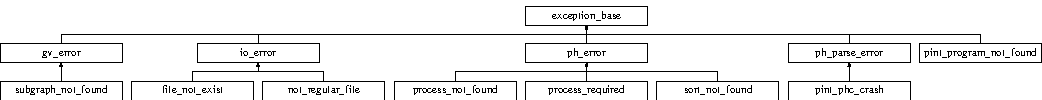
\includegraphics[height=1.337580cm]{structexception__base}
\end{center}
\end{figure}


\subsection{\-Detailed \-Description}
struct defining the base of the exception 

\-The documentation for this class was generated from the following file\-:\begin{DoxyCompactItemize}
\item 
headers/\hyperlink{_exceptions_8h}{\-Exceptions.\-h}\end{DoxyCompactItemize}

\hypertarget{structfile__not__exist}{\section{file\-\_\-not\-\_\-exist \-Class \-Reference}
\label{structfile__not__exist}\index{file\-\_\-not\-\_\-exist@{file\-\_\-not\-\_\-exist}}
}


struct defining the exception called when the file does not exist extends \hyperlink{structio__error}{io\-\_\-error}  




{\ttfamily \#include $<$\-Exceptions.\-h$>$}

\-Inheritance diagram for file\-\_\-not\-\_\-exist\-:\begin{figure}[H]
\begin{center}
\leavevmode
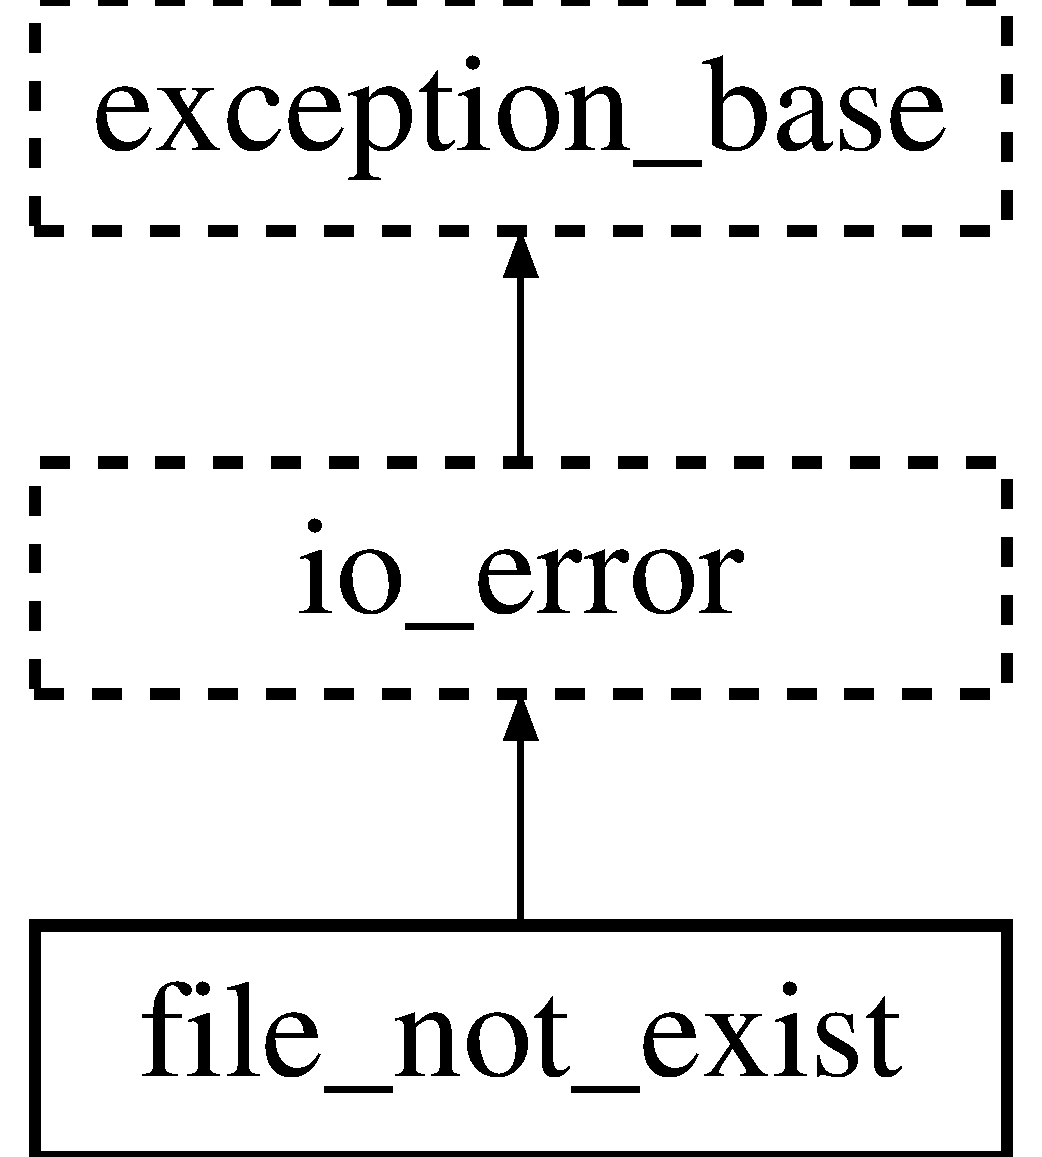
\includegraphics[height=3.000000cm]{structfile__not__exist}
\end{center}
\end{figure}


\subsection{\-Detailed \-Description}
struct defining the exception called when the file does not exist extends \hyperlink{structio__error}{io\-\_\-error} 

\-The documentation for this class was generated from the following file\-:\begin{DoxyCompactItemize}
\item 
headers/\hyperlink{_exceptions_8h}{\-Exceptions.\-h}\end{DoxyCompactItemize}

\hypertarget{class_g_action}{\section{\-G\-Action \-Class \-Reference}
\label{class_g_action}\index{\-G\-Action@{\-G\-Action}}
}


contains style and layout info to draw an action  




{\ttfamily \#include $<$\-G\-Action.\-h$>$}

\subsection*{\-Public \-Member \-Functions}
\begin{DoxyCompactItemize}
\item 
\hyperlink{class_g_action_a697f4b533d191139a1eb401c486afff9}{\-G\-Action} (\-Action\-Ptr a, \hyperlink{struct_g_v_edge}{\-G\-V\-Edge} e, \hyperlink{struct_g_v_edge}{\-G\-V\-Edge} f, \hyperlink{class_p_h_scene}{\-P\-H\-Scene} $\ast$sc)
\begin{DoxyCompactList}\small\item\em constructor \end{DoxyCompactList}\item 
\-Q\-Graphics\-Item $\ast$ \hyperlink{class_g_action_ad3086cca158b494f7c2fd31783fb9f77}{get\-Display\-Item} (void)
\begin{DoxyCompactList}\small\item\em gets the display \end{DoxyCompactList}\item 
\hypertarget{class_g_action_ac9005fd701c1362eea9d7299b95672cb}{\-Action\-Ptr \hyperlink{class_g_action_ac9005fd701c1362eea9d7299b95672cb}{get\-Action} ()}\label{class_g_action_ac9005fd701c1362eea9d7299b95672cb}

\begin{DoxyCompactList}\small\item\em gets the action \end{DoxyCompactList}\item 
\-G\-Sort\-Ptr \hyperlink{class_g_action_a1a76d059cb3b169b5e9dfeed00b41da3}{get\-Source\-Sort} ()
\begin{DoxyCompactList}\small\item\em gets the source \hyperlink{class_g_process}{\-G\-Process} item \end{DoxyCompactList}\item 
\-G\-Sort\-Ptr \hyperlink{class_g_action_a77a2ac1b8a697c066dcf9d6624bb4fa0}{get\-Target\-Sort} ()
\begin{DoxyCompactList}\small\item\em gets the target \hyperlink{class_g_process}{\-G\-Process} item \end{DoxyCompactList}\item 
\-G\-Sort\-Ptr \hyperlink{class_g_action_addc1ebc84b2c739d4fa78d8938f9c6c3}{get\-Result\-Sort} ()
\begin{DoxyCompactList}\small\item\em gets the result \hyperlink{class_g_process}{\-G\-Process} item \end{DoxyCompactList}\end{DoxyCompactItemize}
\subsection*{\-Protected \-Member \-Functions}
\begin{DoxyCompactItemize}
\item 
\-Q\-Graphics\-Polygon\-Item $\ast$ \hyperlink{class_g_action_afeb408bf85d902191cef8a3cf613c7eb}{make\-Arrow\-Head} (const \hyperlink{struct_g_v_edge}{\-G\-V\-Edge} \&e, const \-Q\-Color \&color)
\begin{DoxyCompactList}\small\item\em draws the head of the arrow \end{DoxyCompactList}\end{DoxyCompactItemize}
\subsection*{\-Protected \-Attributes}
\begin{DoxyCompactItemize}
\item 
\hypertarget{class_g_action_a5318deb6935859f5d2ebd1836ec6eb85}{\hyperlink{class_p_h_scene}{\-P\-H\-Scene} $\ast$ \hyperlink{class_g_action_a5318deb6935859f5d2ebd1836ec6eb85}{scene}}\label{class_g_action_a5318deb6935859f5d2ebd1836ec6eb85}

\begin{DoxyCompactList}\small\item\em the \hyperlink{class_p_h_scene}{\-P\-H\-Scene} related to the \hyperlink{class_action}{\-Action} \end{DoxyCompactList}\item 
\hypertarget{class_g_action_a80fd22faf283374dd9861bf4900eafa4}{\-Q\-Graphics\-Item $\ast$ \hyperlink{class_g_action_a80fd22faf283374dd9861bf4900eafa4}{display}}\label{class_g_action_a80fd22faf283374dd9861bf4900eafa4}

\begin{DoxyCompactList}\small\item\em the graphical item representing the \hyperlink{class_action}{\-Action} \end{DoxyCompactList}\item 
\hypertarget{class_g_action_a22f734f6fb2fade298681819341b4f75}{\-Action\-Ptr \hyperlink{class_g_action_a22f734f6fb2fade298681819341b4f75}{action}}\label{class_g_action_a22f734f6fb2fade298681819341b4f75}

\begin{DoxyCompactList}\small\item\em the related \hyperlink{class_action}{\-Action} \end{DoxyCompactList}\item 
\hypertarget{class_g_action_abc626fc7dc52a5f02960706c02a52db9}{pair$<$ \-Q\-Graphics\-Path\-Item \*
$\ast$, \-Q\-Graphics\-Path\-Item $\ast$ $>$ \hyperlink{class_g_action_abc626fc7dc52a5f02960706c02a52db9}{arrow\-Tails}}\label{class_g_action_abc626fc7dc52a5f02960706c02a52db9}

\begin{DoxyCompactList}\small\item\em the pair of graphical items representing the tails of the arrows of the \hyperlink{class_action}{\-Action} \end{DoxyCompactList}\item 
\hypertarget{class_g_action_aab9cc72a8692e0b15f19e192ab21d609}{pair$<$ \-Q\-Graphics\-Polygon\-Item \*
$\ast$, \-Q\-Graphics\-Polygon\-Item $\ast$ $>$ \hyperlink{class_g_action_aab9cc72a8692e0b15f19e192ab21d609}{arrow\-Heads}}\label{class_g_action_aab9cc72a8692e0b15f19e192ab21d609}

\begin{DoxyCompactList}\small\item\em the pair of graphical items representing the heads of the arrows of the \hyperlink{class_action}{\-Action} \end{DoxyCompactList}\item 
\hypertarget{class_g_action_a65f9f4938e024adc07cea387079549f8}{pair$<$ \hyperlink{struct_g_v_edge}{\-G\-V\-Edge}, \hyperlink{struct_g_v_edge}{\-G\-V\-Edge} $>$ \hyperlink{class_g_action_a65f9f4938e024adc07cea387079549f8}{edges}}\label{class_g_action_a65f9f4938e024adc07cea387079549f8}

\begin{DoxyCompactList}\small\item\em the edges related to the arrows \end{DoxyCompactList}\end{DoxyCompactItemize}


\subsection{\-Detailed \-Description}
contains style and layout info to draw an action 

\subsection{\-Constructor \& \-Destructor \-Documentation}
\hypertarget{class_g_action_a697f4b533d191139a1eb401c486afff9}{\index{\-G\-Action@{\-G\-Action}!\-G\-Action@{\-G\-Action}}
\index{\-G\-Action@{\-G\-Action}!GAction@{\-G\-Action}}
\subsubsection[{\-G\-Action}]{\setlength{\rightskip}{0pt plus 5cm}{\bf \-G\-Action\-::\-G\-Action} (
\begin{DoxyParamCaption}
\item[{\-Action\-Ptr}]{a, }
\item[{{\bf \-G\-V\-Edge}}]{e, }
\item[{{\bf \-G\-V\-Edge}}]{f, }
\item[{{\bf \-P\-H\-Scene} $\ast$}]{sc}
\end{DoxyParamCaption}
)}}\label{class_g_action_a697f4b533d191139a1eb401c486afff9}


constructor 


\begin{DoxyParams}{\-Parameters}
{\em \-Action\-Ptr} & the related \hyperlink{class_action}{\-Action} object \\
\hline
{\em \hyperlink{struct_g_v_edge}{\-G\-V\-Edge}} & the object that contains style and layout info for hit arrow \\
\hline
{\em \hyperlink{struct_g_v_edge}{\-G\-V\-Edge}} & the object that contains style and layout info for bounce (result) arrow \\
\hline
{\em \hyperlink{class_p_h_scene}{\-P\-H\-Scene}} & the related scene \\
\hline
\end{DoxyParams}


\subsection{\-Member \-Function \-Documentation}
\hypertarget{class_g_action_ad3086cca158b494f7c2fd31783fb9f77}{\index{\-G\-Action@{\-G\-Action}!get\-Display\-Item@{get\-Display\-Item}}
\index{get\-Display\-Item@{get\-Display\-Item}!GAction@{\-G\-Action}}
\subsubsection[{get\-Display\-Item}]{\setlength{\rightskip}{0pt plus 5cm}\-Q\-Graphics\-Item$\ast$ {\bf \-G\-Action\-::get\-Display\-Item} (
\begin{DoxyParamCaption}
\item[{void}]{}
\end{DoxyParamCaption}
)}}\label{class_g_action_ad3086cca158b494f7c2fd31783fb9f77}


gets the display 

\begin{DoxyReturn}{\-Returns}
\-Q\-Graphics\-Item the graphical item representing the \hyperlink{class_action}{\-Action} 
\end{DoxyReturn}
\hypertarget{class_g_action_addc1ebc84b2c739d4fa78d8938f9c6c3}{\index{\-G\-Action@{\-G\-Action}!get\-Result\-Sort@{get\-Result\-Sort}}
\index{get\-Result\-Sort@{get\-Result\-Sort}!GAction@{\-G\-Action}}
\subsubsection[{get\-Result\-Sort}]{\setlength{\rightskip}{0pt plus 5cm}\-G\-Sort\-Ptr {\bf \-G\-Action\-::get\-Result\-Sort} (
\begin{DoxyParamCaption}
{}
\end{DoxyParamCaption}
)}}\label{class_g_action_addc1ebc84b2c739d4fa78d8938f9c6c3}


gets the result \hyperlink{class_g_process}{\-G\-Process} item 


\begin{DoxyParams}{\-Parameters}
{\em \-G\-Process\-Ptr} & a pointer to the result \hyperlink{class_g_process}{\-G\-Process} item \\
\hline
\end{DoxyParams}
\hypertarget{class_g_action_a1a76d059cb3b169b5e9dfeed00b41da3}{\index{\-G\-Action@{\-G\-Action}!get\-Source\-Sort@{get\-Source\-Sort}}
\index{get\-Source\-Sort@{get\-Source\-Sort}!GAction@{\-G\-Action}}
\subsubsection[{get\-Source\-Sort}]{\setlength{\rightskip}{0pt plus 5cm}\-G\-Sort\-Ptr {\bf \-G\-Action\-::get\-Source\-Sort} (
\begin{DoxyParamCaption}
{}
\end{DoxyParamCaption}
)}}\label{class_g_action_a1a76d059cb3b169b5e9dfeed00b41da3}


gets the source \hyperlink{class_g_process}{\-G\-Process} item 


\begin{DoxyParams}{\-Parameters}
{\em \-G\-Process\-Ptr} & a pointer to the source \hyperlink{class_g_process}{\-G\-Process} item \\
\hline
\end{DoxyParams}
\hypertarget{class_g_action_a77a2ac1b8a697c066dcf9d6624bb4fa0}{\index{\-G\-Action@{\-G\-Action}!get\-Target\-Sort@{get\-Target\-Sort}}
\index{get\-Target\-Sort@{get\-Target\-Sort}!GAction@{\-G\-Action}}
\subsubsection[{get\-Target\-Sort}]{\setlength{\rightskip}{0pt plus 5cm}\-G\-Sort\-Ptr {\bf \-G\-Action\-::get\-Target\-Sort} (
\begin{DoxyParamCaption}
{}
\end{DoxyParamCaption}
)}}\label{class_g_action_a77a2ac1b8a697c066dcf9d6624bb4fa0}


gets the target \hyperlink{class_g_process}{\-G\-Process} item 


\begin{DoxyParams}{\-Parameters}
{\em \-G\-Process\-Ptr} & a pointer to the target \hyperlink{class_g_process}{\-G\-Process} item \\
\hline
\end{DoxyParams}
\hypertarget{class_g_action_afeb408bf85d902191cef8a3cf613c7eb}{\index{\-G\-Action@{\-G\-Action}!make\-Arrow\-Head@{make\-Arrow\-Head}}
\index{make\-Arrow\-Head@{make\-Arrow\-Head}!GAction@{\-G\-Action}}
\subsubsection[{make\-Arrow\-Head}]{\setlength{\rightskip}{0pt plus 5cm}\-Q\-Graphics\-Polygon\-Item$\ast$ {\bf \-G\-Action\-::make\-Arrow\-Head} (
\begin{DoxyParamCaption}
\item[{const {\bf \-G\-V\-Edge} \&}]{e, }
\item[{const \-Q\-Color \&}]{color}
\end{DoxyParamCaption}
)\hspace{0.3cm}{\ttfamily  \mbox{[}protected\mbox{]}}}}\label{class_g_action_afeb408bf85d902191cef8a3cf613c7eb}


draws the head of the arrow 


\begin{DoxyParams}{\-Parameters}
{\em \hyperlink{struct_g_v_edge}{\-G\-V\-Edge}} & the edge related to the arrow \\
\hline
{\em \-Qcolor} & the color of the arrow\\
\hline
\end{DoxyParams}
\begin{DoxyReturn}{\-Returns}
\-Q\-Graphics\-Polygon\-Item$\ast$ the graphical item representing the head of the arrow 
\end{DoxyReturn}


\-The documentation for this class was generated from the following file\-:\begin{DoxyCompactItemize}
\item 
headers/\hyperlink{_g_action_8h}{\-G\-Action.\-h}\end{DoxyCompactItemize}

\hypertarget{class_g_process}{\section{\-G\-Process \-Class \-Reference}
\label{class_g_process}\index{\-G\-Process@{\-G\-Process}}
}


determines the way to draw a process  




{\ttfamily \#include $<$\-G\-Process.\-h$>$}

\subsection*{\-Public \-Member \-Functions}
\begin{DoxyCompactItemize}
\item 
\hyperlink{class_g_process_a16ff7286ec7b0081a6d2a25f9784460f}{\-G\-Process} (\-Process\-Ptr p, \hyperlink{struct_g_v_node}{\-G\-V\-Node} n)
\begin{DoxyCompactList}\small\item\em builder for \hyperlink{class_g_process}{\-G\-Process} \end{DoxyCompactList}\item 
\-Q\-Graphics\-Item $\ast$ \hyperlink{class_g_process_abc8cdf8bb0a8402a1b507005be3a97f9}{get\-Display\-Item} (void)
\begin{DoxyCompactList}\small\item\em getter for the whole drawing of the process \end{DoxyCompactList}\end{DoxyCompactItemize}
\subsection*{\-Protected \-Attributes}
\begin{DoxyCompactItemize}
\item 
\hypertarget{class_g_process_afcb6a6765219d5ca69f23b89a147a7db}{\-Q\-Graphics\-Item $\ast$ \hyperlink{class_g_process_afcb6a6765219d5ca69f23b89a147a7db}{display}}\label{class_g_process_afcb6a6765219d5ca69f23b89a147a7db}

\begin{DoxyCompactList}\small\item\em contains the whole drawing of the process \end{DoxyCompactList}\item 
\hypertarget{class_g_process_ac0770d84d26f835cd409cb1bbd5a2408}{\-Q\-Graphics\-Ellipse\-Item $\ast$ \hyperlink{class_g_process_ac0770d84d26f835cd409cb1bbd5a2408}{ellipse}}\label{class_g_process_ac0770d84d26f835cd409cb1bbd5a2408}

\begin{DoxyCompactList}\small\item\em graphical element to draw the action\-: ellipse \end{DoxyCompactList}\item 
\hypertarget{class_g_process_a4ff36f4f6daae75d094c53d837ad4ecc}{\-Q\-Graphics\-Text\-Item $\ast$ \hyperlink{class_g_process_a4ff36f4f6daae75d094c53d837ad4ecc}{text}}\label{class_g_process_a4ff36f4f6daae75d094c53d837ad4ecc}

\begin{DoxyCompactList}\small\item\em graphical element to draw the action\-: text \end{DoxyCompactList}\item 
\hypertarget{class_g_process_adb2d4b43a105c00b5be1f5bc405a3f43}{\-Process\-Ptr \hyperlink{class_g_process_adb2d4b43a105c00b5be1f5bc405a3f43}{process}}\label{class_g_process_adb2d4b43a105c00b5be1f5bc405a3f43}

\begin{DoxyCompactList}\small\item\em process related \end{DoxyCompactList}\item 
\hypertarget{class_g_process_a83a9972757f06e9eff7fe120ac9f2b5b}{\hyperlink{struct_g_v_node}{\-G\-V\-Node} \hyperlink{class_g_process_a83a9972757f06e9eff7fe120ac9f2b5b}{node}}\label{class_g_process_a83a9972757f06e9eff7fe120ac9f2b5b}

\begin{DoxyCompactList}\small\item\em node related \end{DoxyCompactList}\end{DoxyCompactItemize}


\subsection{\-Detailed \-Description}
determines the way to draw a process 

\subsection{\-Constructor \& \-Destructor \-Documentation}
\hypertarget{class_g_process_a16ff7286ec7b0081a6d2a25f9784460f}{\index{\-G\-Process@{\-G\-Process}!\-G\-Process@{\-G\-Process}}
\index{\-G\-Process@{\-G\-Process}!GProcess@{\-G\-Process}}
\subsubsection[{\-G\-Process}]{\setlength{\rightskip}{0pt plus 5cm}{\bf \-G\-Process\-::\-G\-Process} (
\begin{DoxyParamCaption}
\item[{\-Process\-Ptr}]{p, }
\item[{{\bf \-G\-V\-Node}}]{n}
\end{DoxyParamCaption}
)}}\label{class_g_process_a16ff7286ec7b0081a6d2a25f9784460f}


builder for \hyperlink{class_g_process}{\-G\-Process} 


\begin{DoxyParams}{\-Parameters}
{\em \-Process\-Ptr} & the \hyperlink{class_process}{\-Process} object that will be agregated \\
\hline
{\em \hyperlink{struct_g_v_node}{\-G\-V\-Node}} & the \hyperlink{struct_g_v_node}{\-G\-V\-Node} object that will be agregated \\
\hline
\end{DoxyParams}


\subsection{\-Member \-Function \-Documentation}
\hypertarget{class_g_process_abc8cdf8bb0a8402a1b507005be3a97f9}{\index{\-G\-Process@{\-G\-Process}!get\-Display\-Item@{get\-Display\-Item}}
\index{get\-Display\-Item@{get\-Display\-Item}!GProcess@{\-G\-Process}}
\subsubsection[{get\-Display\-Item}]{\setlength{\rightskip}{0pt plus 5cm}\-Q\-Graphics\-Item$\ast$ {\bf \-G\-Process\-::get\-Display\-Item} (
\begin{DoxyParamCaption}
\item[{void}]{}
\end{DoxyParamCaption}
)}}\label{class_g_process_abc8cdf8bb0a8402a1b507005be3a97f9}


getter for the whole drawing of the process 

\begin{DoxyReturn}{\-Returns}
\-Q\-Graphics\-Item$\ast$ representing the whole drawing of the process 
\end{DoxyReturn}


\-The documentation for this class was generated from the following file\-:\begin{DoxyCompactItemize}
\item 
headers/\hyperlink{_g_process_8h}{\-G\-Process.\-h}\end{DoxyCompactItemize}

\hypertarget{class_g_sort}{\section{\-G\-Sort \-Class \-Reference}
\label{class_g_sort}\index{\-G\-Sort@{\-G\-Sort}}
}


contains style and layout info to draw a \hyperlink{class_sort}{\-Sort}  




{\ttfamily \#include $<$\-G\-Sort.\-h$>$}

\subsection*{\-Public \-Member \-Functions}
\begin{DoxyCompactItemize}
\item 
\hyperlink{class_g_sort_a423709cc4cc15bc05219b08e1276f455}{\-G\-Sort} (\-Sort\-Ptr p, \hyperlink{struct_g_v_cluster}{\-G\-V\-Cluster} c)
\begin{DoxyCompactList}\small\item\em constructor \end{DoxyCompactList}\item 
\hypertarget{class_g_sort_a62b1a8ada691f61cb100568bf25f78d6}{\-Q\-Graphics\-Rect\-Item $\ast$ \hyperlink{class_g_sort_a62b1a8ada691f61cb100568bf25f78d6}{get\-Rect} ()}\label{class_g_sort_a62b1a8ada691f61cb100568bf25f78d6}

\begin{DoxyCompactList}\small\item\em get the rect item \end{DoxyCompactList}\item 
void \hyperlink{class_g_sort_ac3cbef2a811660668cff937f56ca37fe}{mouse\-Press\-Event} (\-Q\-Graphics\-Scene\-Mouse\-Event $\ast$event)
\begin{DoxyCompactList}\small\item\em \-Handles mouse press event (handles drag start) \end{DoxyCompactList}\item 
void \hyperlink{class_g_sort_aad29bd2ba170cd9b89ca80edf3439367}{mouse\-Move\-Event} (\-Q\-Graphics\-Scene\-Mouse\-Event $\ast$event)
\begin{DoxyCompactList}\small\item\em \-Handles mouse move event (handles drag) \end{DoxyCompactList}\item 
void \hyperlink{class_g_sort_a340c92716c90ad010232fdd972902ff0}{mouse\-Release\-Event} (\-Q\-Graphics\-Scene\-Mouse\-Event $\ast$event)
\begin{DoxyCompactList}\small\item\em \-Handles mouse release event (handles drop) \end{DoxyCompactList}\item 
void \hyperlink{class_g_sort_ae7183314fea0d5a3d9a302004d0614a7}{context\-Menu\-Event} (\-Q\-Graphics\-Scene\-Context\-Menu\-Event $\ast$event)
\begin{DoxyCompactList}\small\item\em \-Handles context menu event (typically on right click) \end{DoxyCompactList}\item 
\-Sort\-Ptr \hyperlink{class_g_sort_a69520d78ab078c083b8090f9190424b0}{get\-Sort} ()
\begin{DoxyCompactList}\small\item\em gets the related \hyperlink{class_sort}{\-Sort} object \end{DoxyCompactList}\item 
\hyperlink{struct_g_v_cluster}{\-G\-V\-Cluster} \hyperlink{class_g_sort_ad843ded0ec50cef488015b82661991ed}{get\-Cluster} ()
\begin{DoxyCompactList}\small\item\em gets the related \hyperlink{struct_g_v_cluster}{\-G\-V\-Cluster} which stores \hyperlink{class_g_sort}{\-G\-Sort} absolute coordinates \end{DoxyCompactList}\item 
\hypertarget{class_g_sort_a4ea434778eaf6e7a6dc3603dc1076bb1}{\-Q\-Graphics\-Text\-Item $\ast$ \hyperlink{class_g_sort_a4ea434778eaf6e7a6dc3603dc1076bb1}{get\-Text} ()}\label{class_g_sort_a4ea434778eaf6e7a6dc3603dc1076bb1}

\begin{DoxyCompactList}\small\item\em gets the text of the sort \end{DoxyCompactList}\item 
\hypertarget{class_g_sort_a75e1763370c73d2afbe3727f2742bfa4}{void \hyperlink{class_g_sort_a75e1763370c73d2afbe3727f2742bfa4}{update\-Position} ()}\label{class_g_sort_a75e1763370c73d2afbe3727f2742bfa4}

\begin{DoxyCompactList}\small\item\em updates the position of this \hyperlink{class_g_sort}{\-G\-Sort} after drag\&drop \end{DoxyCompactList}\item 
\hypertarget{class_g_sort_acafeaec8637b62aea47c2ecb4c36e0be}{void \hyperlink{class_g_sort_acafeaec8637b62aea47c2ecb4c36e0be}{hide} ()}\label{class_g_sort_acafeaec8637b62aea47c2ecb4c36e0be}

\begin{DoxyCompactList}\small\item\em hides this \hyperlink{class_g_sort}{\-G\-Sort} setting opacity to 0 \end{DoxyCompactList}\item 
\hypertarget{class_g_sort_a6cb13a9b6ef35dc7698b165ff0d34b88}{void \hyperlink{class_g_sort_a6cb13a9b6ef35dc7698b165ff0d34b88}{show} ()}\label{class_g_sort_a6cb13a9b6ef35dc7698b165ff0d34b88}

\begin{DoxyCompactList}\small\item\em show the \hyperlink{class_g_sort}{\-G\-Sort} setting full opacity \end{DoxyCompactList}\item 
\hypertarget{class_g_sort_a58e2a6099a59b26ffe7dafd90590bd3d}{bool \hyperlink{class_g_sort_a58e2a6099a59b26ffe7dafd90590bd3d}{is\-Visible} ()}\label{class_g_sort_a58e2a6099a59b26ffe7dafd90590bd3d}

\begin{DoxyCompactList}\small\item\em indicates whether or not this \hyperlink{class_g_sort}{\-G\-Sort} is made visible (test based on opacity, cf. \hyperlink{class_g_sort_acafeaec8637b62aea47c2ecb4c36e0be}{hide()} and \hyperlink{class_g_sort_a6cb13a9b6ef35dc7698b165ff0d34b88}{show()}) \end{DoxyCompactList}\end{DoxyCompactItemize}
\subsection*{\-Public \-Attributes}
\begin{DoxyCompactItemize}
\item 
\hypertarget{class_g_sort_afdedfe6a6028c586a755315351eee309}{\-Q\-Color $\ast$ \hyperlink{class_g_sort_afdedfe6a6028c586a755315351eee309}{color}}\label{class_g_sort_afdedfe6a6028c586a755315351eee309}

\begin{DoxyCompactList}\small\item\em the color used by the \-Actions that have this \hyperlink{class_sort}{\-Sort} as source \end{DoxyCompactList}\end{DoxyCompactItemize}
\subsection*{\-Static \-Protected \-Member \-Functions}
\begin{DoxyCompactItemize}
\item 
static \-Q\-Color $\ast$ \hyperlink{class_g_sort_a03da0205abd58bad6c4a58419cb40568}{make\-Color} (void)
\begin{DoxyCompactList}\small\item\em gets a new color in the palette \end{DoxyCompactList}\end{DoxyCompactItemize}
\subsection*{\-Protected \-Attributes}
\begin{DoxyCompactItemize}
\item 
\hypertarget{class_g_sort_aa5979b4b0c0e9efbccce0de13ded38d8}{\-Q\-Graphics\-Rect\-Item $\ast$ \hyperlink{class_g_sort_aa5979b4b0c0e9efbccce0de13ded38d8}{\-\_\-rect}}\label{class_g_sort_aa5979b4b0c0e9efbccce0de13ded38d8}

\begin{DoxyCompactList}\small\item\em the graphical item representing the rectangle of the \hyperlink{class_sort}{\-Sort} \end{DoxyCompactList}\item 
\hypertarget{class_g_sort_a17c4f8eafc9402f5393e69e614f5429a}{\-Q\-Graphics\-Text\-Item $\ast$ \hyperlink{class_g_sort_a17c4f8eafc9402f5393e69e614f5429a}{text}}\label{class_g_sort_a17c4f8eafc9402f5393e69e614f5429a}

\begin{DoxyCompactList}\small\item\em the graphical item representing the text of the \hyperlink{class_sort}{\-Sort} \end{DoxyCompactList}\item 
\hypertarget{class_g_sort_a8dea499c0b3fa30f9e9558a165a52030}{\-Sort\-Ptr \hyperlink{class_g_sort_a8dea499c0b3fa30f9e9558a165a52030}{sort}}\label{class_g_sort_a8dea499c0b3fa30f9e9558a165a52030}

\begin{DoxyCompactList}\small\item\em the related \hyperlink{class_sort}{\-Sort} \end{DoxyCompactList}\item 
\hypertarget{class_g_sort_aed2a99e461d0af9b2b323e1a9fda92fa}{\hyperlink{struct_g_v_cluster}{\-G\-V\-Cluster} \hyperlink{class_g_sort_aed2a99e461d0af9b2b323e1a9fda92fa}{cluster}}\label{class_g_sort_aed2a99e461d0af9b2b323e1a9fda92fa}

\begin{DoxyCompactList}\small\item\em the related cluster \end{DoxyCompactList}\item 
\hypertarget{class_g_sort_a0985310dc8c415f5ac015cde3a28d6a3}{\-Q\-Point \hyperlink{class_g_sort_a0985310dc8c415f5ac015cde3a28d6a3}{init\-Pos\-Point}}\label{class_g_sort_a0985310dc8c415f5ac015cde3a28d6a3}

\begin{DoxyCompactList}\small\item\em the point used to record this \hyperlink{class_g_sort}{\-G\-Sort}'s coordinates when user clicks it (ie. starts drag\&drop) \end{DoxyCompactList}\item 
\hypertarget{class_g_sort_ad33260958b9f1fdea916b737dedc5ba7}{\-Q\-Point \hyperlink{class_g_sort_ad33260958b9f1fdea916b737dedc5ba7}{event\-Press\-Point}}\label{class_g_sort_ad33260958b9f1fdea916b737dedc5ba7}

\begin{DoxyCompactList}\small\item\em the point used to record mouse press event position \end{DoxyCompactList}\item 
\hypertarget{class_g_sort_a92702d91a49f5a4aadf387e6b10c664a}{qreal \hyperlink{class_g_sort_a92702d91a49f5a4aadf387e6b10c664a}{padding\-Top}}\label{class_g_sort_a92702d91a49f5a4aadf387e6b10c664a}

\begin{DoxyCompactList}\small\item\em the space between this \hyperlink{class_g_sort}{\-G\-Sort}'s top side and the top \hyperlink{class_g_process}{\-G\-Process} \end{DoxyCompactList}\end{DoxyCompactItemize}
\subsection*{\-Static \-Protected \-Attributes}
\begin{DoxyCompactItemize}
\item 
\hypertarget{class_g_sort_a575406f7f0f4ce8da65e3456b7fff818}{static std\-::vector$<$ \-Q\-Color $>$ \hyperlink{class_g_sort_a575406f7f0f4ce8da65e3456b7fff818}{palette}}\label{class_g_sort_a575406f7f0f4ce8da65e3456b7fff818}

\begin{DoxyCompactList}\small\item\em the palette of colors that may be used as color member \end{DoxyCompactList}\item 
\hypertarget{class_g_sort_a684c424c03a77a4f60b88f98021bb2eb}{static int \hyperlink{class_g_sort_a684c424c03a77a4f60b88f98021bb2eb}{palette\-Index}}\label{class_g_sort_a684c424c03a77a4f60b88f98021bb2eb}

\begin{DoxyCompactList}\small\item\em palette management index \end{DoxyCompactList}\end{DoxyCompactItemize}


\subsection{\-Detailed \-Description}
contains style and layout info to draw a \hyperlink{class_sort}{\-Sort} 

\subsection{\-Constructor \& \-Destructor \-Documentation}
\hypertarget{class_g_sort_a423709cc4cc15bc05219b08e1276f455}{\index{\-G\-Sort@{\-G\-Sort}!\-G\-Sort@{\-G\-Sort}}
\index{\-G\-Sort@{\-G\-Sort}!GSort@{\-G\-Sort}}
\subsubsection[{\-G\-Sort}]{\setlength{\rightskip}{0pt plus 5cm}{\bf \-G\-Sort\-::\-G\-Sort} (
\begin{DoxyParamCaption}
\item[{\-Sort\-Ptr}]{p, }
\item[{{\bf \-G\-V\-Cluster}}]{c}
\end{DoxyParamCaption}
)}}\label{class_g_sort_a423709cc4cc15bc05219b08e1276f455}


constructor 


\begin{DoxyParams}{\-Parameters}
{\em \-Sort\-Ptr} & the related \hyperlink{class_sort}{\-Sort} object \\
\hline
{\em \hyperlink{struct_g_v_cluster}{\-G\-V\-Cluster}} & the object that contains style and layout info \\
\hline
\end{DoxyParams}


\subsection{\-Member \-Function \-Documentation}
\hypertarget{class_g_sort_ae7183314fea0d5a3d9a302004d0614a7}{\index{\-G\-Sort@{\-G\-Sort}!context\-Menu\-Event@{context\-Menu\-Event}}
\index{context\-Menu\-Event@{context\-Menu\-Event}!GSort@{\-G\-Sort}}
\subsubsection[{context\-Menu\-Event}]{\setlength{\rightskip}{0pt plus 5cm}void {\bf \-G\-Sort\-::context\-Menu\-Event} (
\begin{DoxyParamCaption}
\item[{\-Q\-Graphics\-Scene\-Context\-Menu\-Event $\ast$}]{event}
\end{DoxyParamCaption}
)}}\label{class_g_sort_ae7183314fea0d5a3d9a302004d0614a7}


\-Handles context menu event (typically on right click) 


\begin{DoxyParams}{\-Parameters}
{\em \-Q\-Graphics\-Scene\-Context\-Menu\-Event} & the event to be handled \\
\hline
\end{DoxyParams}
\hypertarget{class_g_sort_ad843ded0ec50cef488015b82661991ed}{\index{\-G\-Sort@{\-G\-Sort}!get\-Cluster@{get\-Cluster}}
\index{get\-Cluster@{get\-Cluster}!GSort@{\-G\-Sort}}
\subsubsection[{get\-Cluster}]{\setlength{\rightskip}{0pt plus 5cm}{\bf \-G\-V\-Cluster} {\bf \-G\-Sort\-::get\-Cluster} (
\begin{DoxyParamCaption}
{}
\end{DoxyParamCaption}
)}}\label{class_g_sort_ad843ded0ec50cef488015b82661991ed}


gets the related \hyperlink{struct_g_v_cluster}{\-G\-V\-Cluster} which stores \hyperlink{class_g_sort}{\-G\-Sort} absolute coordinates 

\begin{DoxyReturn}{\-Returns}
\hyperlink{struct_g_v_cluster}{\-G\-V\-Cluster} the related \hyperlink{struct_g_v_cluster}{\-G\-V\-Cluster} 
\end{DoxyReturn}
\hypertarget{class_g_sort_a69520d78ab078c083b8090f9190424b0}{\index{\-G\-Sort@{\-G\-Sort}!get\-Sort@{get\-Sort}}
\index{get\-Sort@{get\-Sort}!GSort@{\-G\-Sort}}
\subsubsection[{get\-Sort}]{\setlength{\rightskip}{0pt plus 5cm}\-Sort\-Ptr {\bf \-G\-Sort\-::get\-Sort} (
\begin{DoxyParamCaption}
{}
\end{DoxyParamCaption}
)}}\label{class_g_sort_a69520d78ab078c083b8090f9190424b0}


gets the related \hyperlink{class_sort}{\-Sort} object 

\begin{DoxyReturn}{\-Returns}
\-Sort\-Ptr a pointer to the related \hyperlink{class_sort}{\-Sort} object 
\end{DoxyReturn}
\hypertarget{class_g_sort_a03da0205abd58bad6c4a58419cb40568}{\index{\-G\-Sort@{\-G\-Sort}!make\-Color@{make\-Color}}
\index{make\-Color@{make\-Color}!GSort@{\-G\-Sort}}
\subsubsection[{make\-Color}]{\setlength{\rightskip}{0pt plus 5cm}static \-Q\-Color$\ast$ {\bf \-G\-Sort\-::make\-Color} (
\begin{DoxyParamCaption}
\item[{void}]{}
\end{DoxyParamCaption}
)\hspace{0.3cm}{\ttfamily  \mbox{[}static, protected\mbox{]}}}}\label{class_g_sort_a03da0205abd58bad6c4a58419cb40568}


gets a new color in the palette 

\begin{DoxyReturn}{\-Returns}
\-Q\-Color$\ast$ the color retrieved in the palette 
\end{DoxyReturn}
\hypertarget{class_g_sort_aad29bd2ba170cd9b89ca80edf3439367}{\index{\-G\-Sort@{\-G\-Sort}!mouse\-Move\-Event@{mouse\-Move\-Event}}
\index{mouse\-Move\-Event@{mouse\-Move\-Event}!GSort@{\-G\-Sort}}
\subsubsection[{mouse\-Move\-Event}]{\setlength{\rightskip}{0pt plus 5cm}void {\bf \-G\-Sort\-::mouse\-Move\-Event} (
\begin{DoxyParamCaption}
\item[{\-Q\-Graphics\-Scene\-Mouse\-Event $\ast$}]{event}
\end{DoxyParamCaption}
)}}\label{class_g_sort_aad29bd2ba170cd9b89ca80edf3439367}


\-Handles mouse move event (handles drag) 


\begin{DoxyParams}{\-Parameters}
{\em \-Q\-Graphics\-Scene\-Mouse\-Event} & the event to be handled \\
\hline
\end{DoxyParams}
\hypertarget{class_g_sort_ac3cbef2a811660668cff937f56ca37fe}{\index{\-G\-Sort@{\-G\-Sort}!mouse\-Press\-Event@{mouse\-Press\-Event}}
\index{mouse\-Press\-Event@{mouse\-Press\-Event}!GSort@{\-G\-Sort}}
\subsubsection[{mouse\-Press\-Event}]{\setlength{\rightskip}{0pt plus 5cm}void {\bf \-G\-Sort\-::mouse\-Press\-Event} (
\begin{DoxyParamCaption}
\item[{\-Q\-Graphics\-Scene\-Mouse\-Event $\ast$}]{event}
\end{DoxyParamCaption}
)}}\label{class_g_sort_ac3cbef2a811660668cff937f56ca37fe}


\-Handles mouse press event (handles drag start) 


\begin{DoxyParams}{\-Parameters}
{\em \-Q\-Graphics\-Scene\-Mouse\-Event} & the event to be handled \\
\hline
\end{DoxyParams}
\hypertarget{class_g_sort_a340c92716c90ad010232fdd972902ff0}{\index{\-G\-Sort@{\-G\-Sort}!mouse\-Release\-Event@{mouse\-Release\-Event}}
\index{mouse\-Release\-Event@{mouse\-Release\-Event}!GSort@{\-G\-Sort}}
\subsubsection[{mouse\-Release\-Event}]{\setlength{\rightskip}{0pt plus 5cm}void {\bf \-G\-Sort\-::mouse\-Release\-Event} (
\begin{DoxyParamCaption}
\item[{\-Q\-Graphics\-Scene\-Mouse\-Event $\ast$}]{event}
\end{DoxyParamCaption}
)}}\label{class_g_sort_a340c92716c90ad010232fdd972902ff0}


\-Handles mouse release event (handles drop) 


\begin{DoxyParams}{\-Parameters}
{\em \-Q\-Graphics\-Scene\-Mouse\-Event} & the event to be handled \\
\hline
\end{DoxyParams}


\-The documentation for this class was generated from the following file\-:\begin{DoxyCompactItemize}
\item 
headers/\hyperlink{_g_sort_8h}{\-G\-Sort.\-h}\end{DoxyCompactItemize}

\hypertarget{structgv__error}{\section{gv\-\_\-error \-Class \-Reference}
\label{structgv__error}\index{gv\-\_\-error@{gv\-\_\-error}}
}


struct defining the exception called when an error occurs in \-Graph\-Viz extends \hyperlink{structexception__base}{exception\-\_\-base}  




{\ttfamily \#include $<$\-Exceptions.\-h$>$}

\-Inheritance diagram for gv\-\_\-error\-:\begin{figure}[H]
\begin{center}
\leavevmode
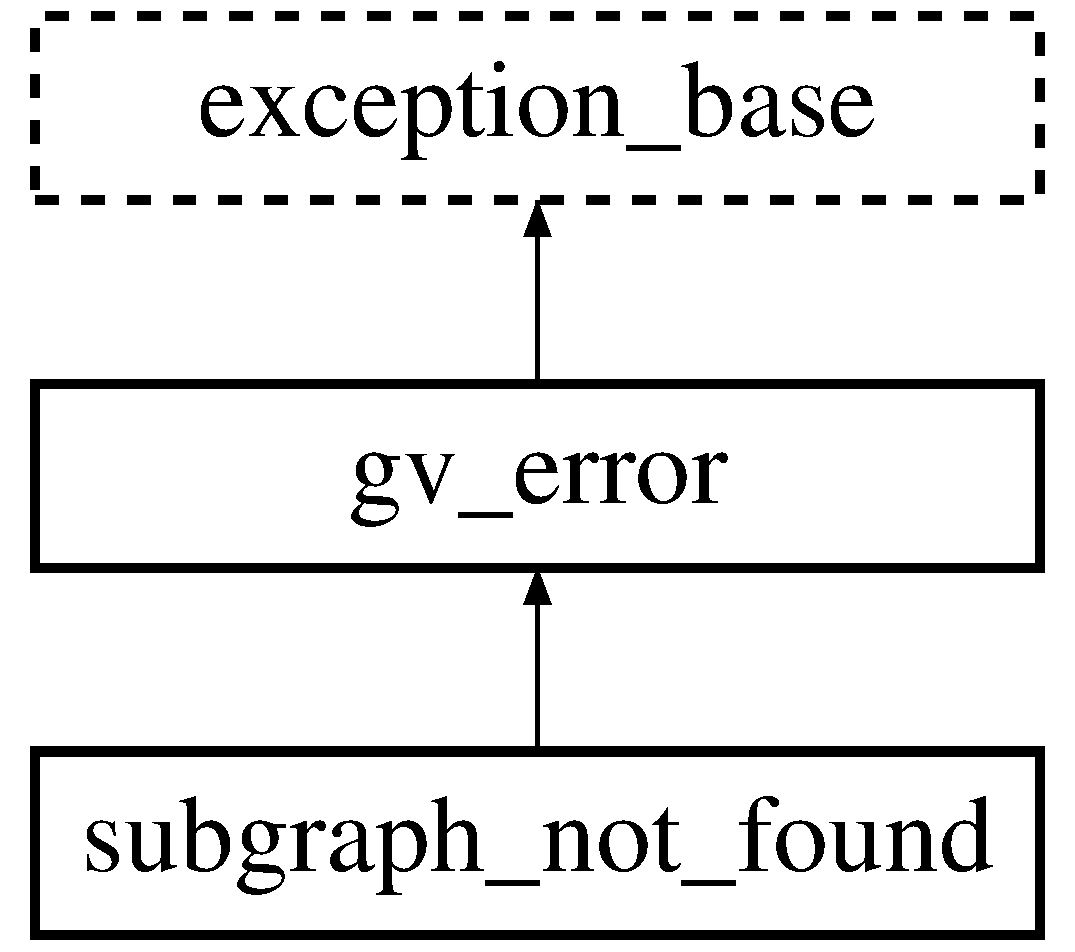
\includegraphics[height=3.000000cm]{structgv__error}
\end{center}
\end{figure}


\subsection{\-Detailed \-Description}
struct defining the exception called when an error occurs in \-Graph\-Viz extends \hyperlink{structexception__base}{exception\-\_\-base} 

\-The documentation for this class was generated from the following file\-:\begin{DoxyCompactItemize}
\item 
headers/\hyperlink{_exceptions_8h}{\-Exceptions.\-h}\end{DoxyCompactItemize}

\hypertarget{struct_g_v_cluster}{\section{\-G\-V\-Cluster \-Struct \-Reference}
\label{struct_g_v_cluster}\index{\-G\-V\-Cluster@{\-G\-V\-Cluster}}
}


struct containing the information for a \hyperlink{class_g_v_graph}{\-G\-V\-Graph}'s node  




{\ttfamily \#include $<$\-G\-V\-Cluster.\-h$>$}

\subsection*{\-Public \-Attributes}
\begin{DoxyCompactItemize}
\item 
\hypertarget{struct_g_v_cluster_a24bc2aff9c2fb442ecdf2beea9149083}{\-Q\-String \hyperlink{struct_g_v_cluster_a24bc2aff9c2fb442ecdf2beea9149083}{name}}\label{struct_g_v_cluster_a24bc2aff9c2fb442ecdf2beea9149083}

\begin{DoxyCompactList}\small\item\em the unique identifier of the cluster in the graph \end{DoxyCompactList}\item 
\hypertarget{struct_g_v_cluster_a14f3667939642696081fa76dadb124a4}{\-Q\-Point \hyperlink{struct_g_v_cluster_a14f3667939642696081fa76dadb124a4}{top\-Left}}\label{struct_g_v_cluster_a14f3667939642696081fa76dadb124a4}

\begin{DoxyCompactList}\small\item\em the position of the top-\/left corner \end{DoxyCompactList}\item 
\hypertarget{struct_g_v_cluster_a2fd97f94a1a92153039dd6a4ac5ba5d4}{float \hyperlink{struct_g_v_cluster_a2fd97f94a1a92153039dd6a4ac5ba5d4}{height}}\label{struct_g_v_cluster_a2fd97f94a1a92153039dd6a4ac5ba5d4}

\begin{DoxyCompactList}\small\item\em the size (height and width) of the cluster in pixels \end{DoxyCompactList}\item 
\hypertarget{struct_g_v_cluster_a88d166bcf31587ac7482c997f0c17f15}{float {\bfseries width}}\label{struct_g_v_cluster_a88d166bcf31587ac7482c997f0c17f15}

\item 
\hypertarget{struct_g_v_cluster_a53d0a695bef9a7231eaba118a859a28f}{\-Q\-Point \hyperlink{struct_g_v_cluster_a53d0a695bef9a7231eaba118a859a28f}{label\-Pos}}\label{struct_g_v_cluster_a53d0a695bef9a7231eaba118a859a28f}

\begin{DoxyCompactList}\small\item\em the label position \end{DoxyCompactList}\end{DoxyCompactItemize}


\subsection{\-Detailed \-Description}
struct containing the information for a \hyperlink{class_g_v_graph}{\-G\-V\-Graph}'s node 

\-The documentation for this struct was generated from the following file\-:\begin{DoxyCompactItemize}
\item 
headers/\hyperlink{_g_v_cluster_8h}{\-G\-V\-Cluster.\-h}\end{DoxyCompactItemize}

\hypertarget{struct_g_v_edge}{\section{\-G\-V\-Edge \-Struct \-Reference}
\label{struct_g_v_edge}\index{\-G\-V\-Edge@{\-G\-V\-Edge}}
}


struct containing the information for a \hyperlink{class_g_v_graph}{\-G\-V\-Graph}'s edge  




{\ttfamily \#include $<$\-G\-V\-Edge.\-h$>$}

\subsection*{\-Public \-Attributes}
\begin{DoxyCompactItemize}
\item 
\hypertarget{struct_g_v_edge_a7a3538b20c3747135ce4771be00a3a8a}{\-Q\-String \hyperlink{struct_g_v_edge_a7a3538b20c3747135ce4771be00a3a8a}{source}}\label{struct_g_v_edge_a7a3538b20c3747135ce4771be00a3a8a}

\begin{DoxyCompactList}\small\item\em the source node of the edge \end{DoxyCompactList}\item 
\hypertarget{struct_g_v_edge_a6883e0ddce3a6fcbde0b01f3645ae7c5}{\-Q\-String \hyperlink{struct_g_v_edge_a6883e0ddce3a6fcbde0b01f3645ae7c5}{target}}\label{struct_g_v_edge_a6883e0ddce3a6fcbde0b01f3645ae7c5}

\begin{DoxyCompactList}\small\item\em the target node of the edge \end{DoxyCompactList}\item 
\hypertarget{struct_g_v_edge_ad73f00af1e82b13f9c94982327bc9952}{\-Q\-Painter\-Path \hyperlink{struct_g_v_edge_ad73f00af1e82b13f9c94982327bc9952}{path}}\label{struct_g_v_edge_ad73f00af1e82b13f9c94982327bc9952}

\begin{DoxyCompactList}\small\item\em the path of the edge's line \end{DoxyCompactList}\end{DoxyCompactItemize}


\subsection{\-Detailed \-Description}
struct containing the information for a \hyperlink{class_g_v_graph}{\-G\-V\-Graph}'s edge 

\-The documentation for this struct was generated from the following file\-:\begin{DoxyCompactItemize}
\item 
headers/\hyperlink{_g_v_edge_8h}{\-G\-V\-Edge.\-h}\end{DoxyCompactItemize}

\hypertarget{class_g_v_graph}{\section{\-G\-V\-Graph \-Class \-Reference}
\label{class_g_v_graph}\index{\-G\-V\-Graph@{\-G\-V\-Graph}}
}


object containing a libgraph graph and its associated nodes and edges  




{\ttfamily \#include $<$\-G\-V\-Graph.\-h$>$}

\-Inheritance diagram for \-G\-V\-Graph\-:\begin{figure}[H]
\begin{center}
\leavevmode
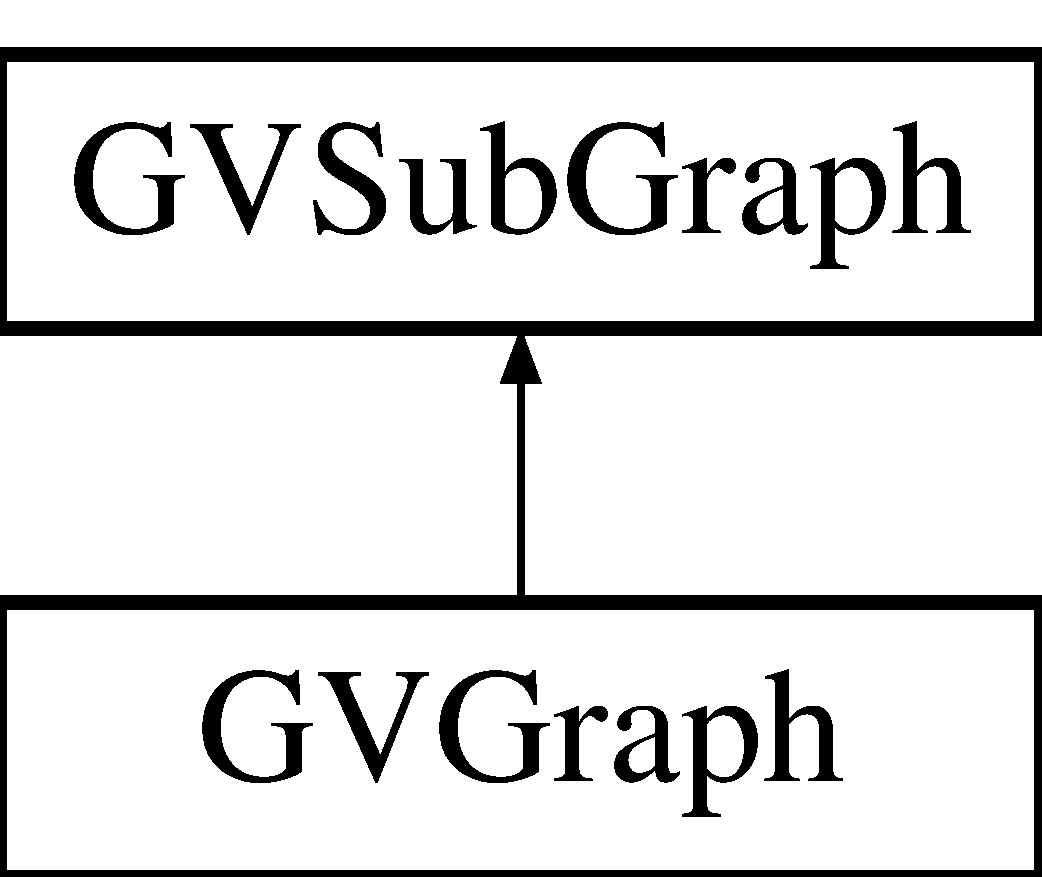
\includegraphics[height=2.000000cm]{class_g_v_graph}
\end{center}
\end{figure}
\subsection*{\-Public \-Member \-Functions}
\begin{DoxyCompactItemize}
\item 
\hyperlink{class_g_v_graph_af47604f64a70e17ba11af26787497fbb}{\-G\-V\-Graph} (\-Q\-String name, \-Q\-Font font=\-Q\-Font())
\begin{DoxyCompactList}\small\item\em \-Construct a \-Graphviz graph object. \end{DoxyCompactList}\item 
\hypertarget{class_g_v_graph_aebfd43267ab4f7cfb46d2841f6b52aeb}{void \hyperlink{class_g_v_graph_aebfd43267ab4f7cfb46d2841f6b52aeb}{apply\-Layout} (void)}\label{class_g_v_graph_aebfd43267ab4f7cfb46d2841f6b52aeb}

\begin{DoxyCompactList}\small\item\em builds the layout \end{DoxyCompactList}\item 
void \hyperlink{class_g_v_graph_a9fee4d22192b53b8b012ed3e72ea92cd}{render\-To\-File} (\-Q\-String name)
\begin{DoxyCompactList}\small\item\em renders the file \end{DoxyCompactList}\item 
\-Q\-Rect\-F \hyperlink{class_g_v_graph_a381255296a418044949c6854699a1f76}{bounding\-Rect} ()
\begin{DoxyCompactList}\small\item\em the rectangle result \end{DoxyCompactList}\item 
void \hyperlink{class_g_v_graph_ae48ac71c72224ac6e6c761fd6e9b3c61}{set\-Font} (\-Q\-Font font)
\begin{DoxyCompactList}\small\item\em sets the font that will be used in all the labels \end{DoxyCompactList}\end{DoxyCompactItemize}
\subsection*{\-Static \-Public \-Attributes}
\begin{DoxyCompactItemize}
\item 
\hypertarget{class_g_v_graph_a643ff39dc5b5aba36f91f0d4d55cdc70}{static const qreal \hyperlink{class_g_v_graph_a643ff39dc5b5aba36f91f0d4d55cdc70}{\-Dot\-Default\-D\-P\-I}}\label{class_g_v_graph_a643ff39dc5b5aba36f91f0d4d55cdc70}

\begin{DoxyCompactList}\small\item\em \-Default \-D\-P\-I value used by dot (which uses points instead of pixels for coordinates) \end{DoxyCompactList}\end{DoxyCompactItemize}


\subsection{\-Detailed \-Description}
object containing a libgraph graph and its associated nodes and edges 

\subsection{\-Constructor \& \-Destructor \-Documentation}
\hypertarget{class_g_v_graph_af47604f64a70e17ba11af26787497fbb}{\index{\-G\-V\-Graph@{\-G\-V\-Graph}!\-G\-V\-Graph@{\-G\-V\-Graph}}
\index{\-G\-V\-Graph@{\-G\-V\-Graph}!GVGraph@{\-G\-V\-Graph}}
\subsubsection[{\-G\-V\-Graph}]{\setlength{\rightskip}{0pt plus 5cm}{\bf \-G\-V\-Graph\-::\-G\-V\-Graph} (
\begin{DoxyParamCaption}
\item[{\-Q\-String}]{name, }
\item[{\-Q\-Font}]{font = {\ttfamily \-Q\-Font()}}
\end{DoxyParamCaption}
)}}\label{class_g_v_graph_af47604f64a70e17ba11af26787497fbb}


\-Construct a \-Graphviz graph object. 


\begin{DoxyParams}{\-Parameters}
{\em name} & \-The name of the graph, must be unique in the application \\
\hline
{\em font} & \-The font to use for the graph \\
\hline
{\em node\-\_\-size} & \-The size in pixels of each node \\
\hline
\end{DoxyParams}


\subsection{\-Member \-Function \-Documentation}
\hypertarget{class_g_v_graph_a381255296a418044949c6854699a1f76}{\index{\-G\-V\-Graph@{\-G\-V\-Graph}!bounding\-Rect@{bounding\-Rect}}
\index{bounding\-Rect@{bounding\-Rect}!GVGraph@{\-G\-V\-Graph}}
\subsubsection[{bounding\-Rect}]{\setlength{\rightskip}{0pt plus 5cm}\-Q\-Rect\-F {\bf \-G\-V\-Graph\-::bounding\-Rect} (
\begin{DoxyParamCaption}
{}
\end{DoxyParamCaption}
)}}\label{class_g_v_graph_a381255296a418044949c6854699a1f76}


the rectangle result 

\begin{DoxyReturn}{\-Returns}
a \-Q\-Rect\-F representing the rectangle built 
\end{DoxyReturn}
\hypertarget{class_g_v_graph_a9fee4d22192b53b8b012ed3e72ea92cd}{\index{\-G\-V\-Graph@{\-G\-V\-Graph}!render\-To\-File@{render\-To\-File}}
\index{render\-To\-File@{render\-To\-File}!GVGraph@{\-G\-V\-Graph}}
\subsubsection[{render\-To\-File}]{\setlength{\rightskip}{0pt plus 5cm}void {\bf \-G\-V\-Graph\-::render\-To\-File} (
\begin{DoxyParamCaption}
\item[{\-Q\-String}]{name}
\end{DoxyParamCaption}
)}}\label{class_g_v_graph_a9fee4d22192b53b8b012ed3e72ea92cd}


renders the file 


\begin{DoxyParams}{\-Parameters}
{\em \-Qstring} & name of the file you want to render \\
\hline
\end{DoxyParams}
\hypertarget{class_g_v_graph_ae48ac71c72224ac6e6c761fd6e9b3c61}{\index{\-G\-V\-Graph@{\-G\-V\-Graph}!set\-Font@{set\-Font}}
\index{set\-Font@{set\-Font}!GVGraph@{\-G\-V\-Graph}}
\subsubsection[{set\-Font}]{\setlength{\rightskip}{0pt plus 5cm}void {\bf \-G\-V\-Graph\-::set\-Font} (
\begin{DoxyParamCaption}
\item[{\-Q\-Font}]{font}
\end{DoxyParamCaption}
)}}\label{class_g_v_graph_ae48ac71c72224ac6e6c761fd6e9b3c61}


sets the font that will be used in all the labels 


\begin{DoxyParams}{\-Parameters}
{\em \-Q\-Font} & chosen to be used \\
\hline
\end{DoxyParams}


\-The documentation for this class was generated from the following file\-:\begin{DoxyCompactItemize}
\item 
headers/\hyperlink{_g_v_graph_8h}{\-G\-V\-Graph.\-h}\end{DoxyCompactItemize}

\hypertarget{struct_g_v_node}{\section{\-G\-V\-Node \-Struct \-Reference}
\label{struct_g_v_node}\index{\-G\-V\-Node@{\-G\-V\-Node}}
}


struct containing the information for a \hyperlink{class_g_v_graph}{\-G\-V\-Graph}'s node  




{\ttfamily \#include $<$\-G\-V\-Node.\-h$>$}

\subsection*{\-Public \-Attributes}
\begin{DoxyCompactItemize}
\item 
\hypertarget{struct_g_v_node_ad1af9e7c14f0b580854ad3428f1b5c9d}{\-Q\-String \hyperlink{struct_g_v_node_ad1af9e7c14f0b580854ad3428f1b5c9d}{name}}\label{struct_g_v_node_ad1af9e7c14f0b580854ad3428f1b5c9d}

\begin{DoxyCompactList}\small\item\em the unique identifier of the node in the graph \end{DoxyCompactList}\item 
\hypertarget{struct_g_v_node_a2ceb3d0e7d3f164710622acd3cbea6a6}{\-Q\-Point \hyperlink{struct_g_v_node_a2ceb3d0e7d3f164710622acd3cbea6a6}{center\-Pos}}\label{struct_g_v_node_a2ceb3d0e7d3f164710622acd3cbea6a6}

\begin{DoxyCompactList}\small\item\em position of the center point of the node from the top-\/left corner \end{DoxyCompactList}\item 
\hypertarget{struct_g_v_node_a498e3f749e2228709a3987ac11512c82}{float \hyperlink{struct_g_v_node_a498e3f749e2228709a3987ac11512c82}{height}}\label{struct_g_v_node_a498e3f749e2228709a3987ac11512c82}

\begin{DoxyCompactList}\small\item\em the size (height and width) of the node in pixels \end{DoxyCompactList}\item 
\hypertarget{struct_g_v_node_adc1d840d0813610c08420ce97195b893}{float {\bfseries width}}\label{struct_g_v_node_adc1d840d0813610c08420ce97195b893}

\end{DoxyCompactItemize}


\subsection{\-Detailed \-Description}
struct containing the information for a \hyperlink{class_g_v_graph}{\-G\-V\-Graph}'s node 

\-The documentation for this struct was generated from the following file\-:\begin{DoxyCompactItemize}
\item 
headers/\hyperlink{_g_v_node_8h}{\-G\-V\-Node.\-h}\end{DoxyCompactItemize}

\hypertarget{class_g_v_sub_graph}{\section{\-G\-V\-Sub\-Graph \-Class \-Reference}
\label{class_g_v_sub_graph}\index{\-G\-V\-Sub\-Graph@{\-G\-V\-Sub\-Graph}}
}


the object containing a libraph subgraph and its associated nodes and edges  




{\ttfamily \#include $<$\-G\-V\-Sub\-Graph.\-h$>$}

\-Inheritance diagram for \-G\-V\-Sub\-Graph\-:\begin{figure}[H]
\begin{center}
\leavevmode
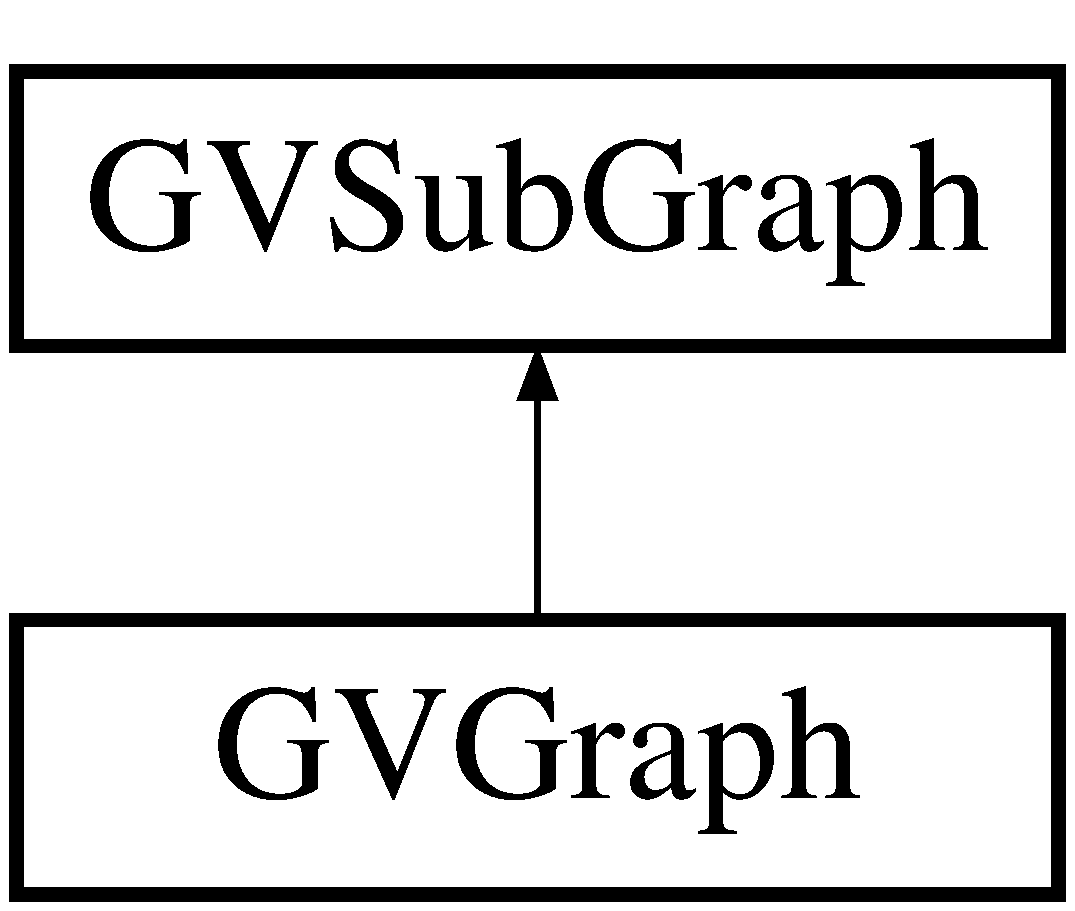
\includegraphics[height=2.000000cm]{class_g_v_sub_graph}
\end{center}
\end{figure}
\subsection*{\-Public \-Member \-Functions}
\begin{DoxyCompactItemize}
\item 
\hyperlink{class_g_v_sub_graph_a2a830f5288096466cff627fb221003f3}{\-G\-V\-Sub\-Graph} (\-Agraph\-\_\-t $\ast$\hyperlink{class_g_v_sub_graph_ae9ba380851ecbc611bbe9cd2980ba152}{\-\_\-graph})
\begin{DoxyCompactList}\small\item\em \hyperlink{class_g_v_sub_graph}{\-G\-V\-Sub\-Graph} constructor. \end{DoxyCompactList}\item 
void \hyperlink{class_g_v_sub_graph_a7999f5541dde4ad692b8f1765675e106}{add\-Sub\-Graph} (const \-Q\-String \&name)
\begin{DoxyCompactList}\small\item\em adds a subgraph \end{DoxyCompactList}\item 
void \hyperlink{class_g_v_sub_graph_a1bed9f509bbe210754ed6e2878a75dff}{remove\-Sub\-Graph} (const \-Q\-String \&name)
\begin{DoxyCompactList}\small\item\em removes a subgraph \end{DoxyCompactList}\item 
\-G\-V\-Sub\-Graph\-Ptr \hyperlink{class_g_v_sub_graph_abfbc0deb675aaf2e0bf0551b17506818}{get\-Sub\-Graph} (const \-Q\-String \&name)
\begin{DoxyCompactList}\small\item\em retrieves a \hyperlink{class_g_v_sub_graph}{\-G\-V\-Sub\-Graph} by its name \end{DoxyCompactList}\item 
int \hyperlink{class_g_v_sub_graph_af0087db5d9f5a53132f1b46b636377f9}{count\-Nodes} (void)
\begin{DoxyCompactList}\small\item\em counts the number of nodes \end{DoxyCompactList}\item 
void \hyperlink{class_g_v_sub_graph_a99ea8e4c658ea76fc5425644a460362d}{add\-Node} (const \-Q\-String \&name)
\begin{DoxyCompactList}\small\item\em adds a node, entering its name \end{DoxyCompactList}\item 
void \hyperlink{class_g_v_sub_graph_af805b3fbfb96c0b1cb99ecc311f1a7f8}{add\-Nodes} (const \-Q\-String\-List \&names)
\begin{DoxyCompactList}\small\item\em adds a list of nodes, entering their names \end{DoxyCompactList}\item 
void \hyperlink{class_g_v_sub_graph_ac97b366dadeeb5ac8999ee6b22dd7dd4}{remove\-Node} (const \-Q\-String \&name)
\begin{DoxyCompactList}\small\item\em removes a node, entering its name \end{DoxyCompactList}\item 
\hypertarget{class_g_v_sub_graph_a57609be587187f492288d224216b3b14}{void \hyperlink{class_g_v_sub_graph_a57609be587187f492288d224216b3b14}{clear\-Nodes} ()}\label{class_g_v_sub_graph_a57609be587187f492288d224216b3b14}

\begin{DoxyCompactList}\small\item\em removes all the nodes \end{DoxyCompactList}\item 
void \hyperlink{class_g_v_sub_graph_a84df91480a9e3c7ec38658b475e13d90}{add\-Edge} (const \-Q\-String \&source, const \-Q\-String \&target)
\begin{DoxyCompactList}\small\item\em adds an edge \end{DoxyCompactList}\item 
void \hyperlink{class_g_v_sub_graph_adeec195e6301f14864ad3cf4ecb2a7e6}{remove\-Edge} (const \-Q\-String \&source, const \-Q\-String \&target)
\begin{DoxyCompactList}\small\item\em removes an edge \end{DoxyCompactList}\item 
void \hyperlink{class_g_v_sub_graph_a42c2d7c92a223e40364c13fdb1cc46e8}{remove\-Edge} (const \-Q\-Pair$<$ \-Q\-String, \-Q\-String $>$ \&key)
\begin{DoxyCompactList}\small\item\em removes an edge, entering the pair (source, target) \end{DoxyCompactList}\item 
void \hyperlink{class_g_v_sub_graph_a14a5e0a85c54220e4908e2692576e62b}{set\-Label} (const \-Q\-String \&name)
\begin{DoxyCompactList}\small\item\em sets the label \end{DoxyCompactList}\item 
\-Q\-List$<$ \hyperlink{struct_g_v_node}{\-G\-V\-Node} $>$ \hyperlink{class_g_v_sub_graph_a777c2146e514db2ccded4b3f77993155}{nodes} ()
\begin{DoxyCompactList}\small\item\em gets the list of nodes \end{DoxyCompactList}\item 
\-Q\-List$<$ \hyperlink{struct_g_v_cluster}{\-G\-V\-Cluster} $>$ \hyperlink{class_g_v_sub_graph_a52594db2f31cfb221820cbd48b6d3530}{clusters} ()
\begin{DoxyCompactList}\small\item\em gets the list of clusters \end{DoxyCompactList}\item 
\-Q\-List$<$ \hyperlink{struct_g_v_edge}{\-G\-V\-Edge} $>$ \hyperlink{class_g_v_sub_graph_a88469fa80e33d2506cde3b6352c3c508}{edges} ()
\begin{DoxyCompactList}\small\item\em gets the list of edges \end{DoxyCompactList}\end{DoxyCompactItemize}
\subsection*{\-Static \-Public \-Attributes}
\begin{DoxyCompactItemize}
\item 
\hypertarget{class_g_v_sub_graph_acad7d627217c64966125e7701142c40b}{static const qreal \hyperlink{class_g_v_sub_graph_acad7d627217c64966125e7701142c40b}{node\-Size}}\label{class_g_v_sub_graph_acad7d627217c64966125e7701142c40b}

\begin{DoxyCompactList}\small\item\em the size in pixels of each node \end{DoxyCompactList}\end{DoxyCompactItemize}
\subsection*{\-Protected \-Member \-Functions}
\begin{DoxyCompactItemize}
\item 
qreal \hyperlink{class_g_v_sub_graph_a0405ca939a02f54ccdf044a5a6f4ff6b}{get\-D\-P\-I} ()
\begin{DoxyCompactList}\small\item\em gets the \-D\-P\-I value \end{DoxyCompactList}\item 
\hypertarget{class_g_v_sub_graph_a6f94775bfde0ef47c59df8a7e6510aaf}{void \hyperlink{class_g_v_sub_graph_a6f94775bfde0ef47c59df8a7e6510aaf}{set\-Graph\-Attributes} (void)}\label{class_g_v_sub_graph_a6f94775bfde0ef47c59df8a7e6510aaf}

\begin{DoxyCompactList}\small\item\em sets the \-Graph \-Attributes \end{DoxyCompactList}\item 
bool \hyperlink{class_g_v_sub_graph_af55511f05fe4d65e122cc77c2d02a706}{has\-Node} (const \-Q\-String \&name)
\begin{DoxyCompactList}\small\item\em checks if the node exists \end{DoxyCompactList}\item 
\-Agnode\-\_\-t $\ast$ \hyperlink{class_g_v_sub_graph_aaa1df9ed6bbd2ea697646e8bbfb571da}{get\-Node} (const \-Q\-String \&name)
\begin{DoxyCompactList}\small\item\em gets a node \end{DoxyCompactList}\end{DoxyCompactItemize}
\subsection*{\-Protected \-Attributes}
\begin{DoxyCompactItemize}
\item 
\hypertarget{class_g_v_sub_graph_ae9ba380851ecbc611bbe9cd2980ba152}{\-Agraph\-\_\-t $\ast$ \hyperlink{class_g_v_sub_graph_ae9ba380851ecbc611bbe9cd2980ba152}{\-\_\-graph}}\label{class_g_v_sub_graph_ae9ba380851ecbc611bbe9cd2980ba152}

\begin{DoxyCompactList}\small\item\em \-Agraph\-\_\-t the related \-Graphviz graph. \end{DoxyCompactList}\item 
\hypertarget{class_g_v_sub_graph_ab994dac998f44c0566567d9cf28c5aae}{\-Q\-Map$<$ \-Q\-String, \-Agnode\-\_\-t $\ast$ $>$ {\bfseries \-\_\-nodes}}\label{class_g_v_sub_graph_ab994dac998f44c0566567d9cf28c5aae}

\item 
\hypertarget{class_g_v_sub_graph_a4bfd077344f6c2c530bb614b347ee7e0}{\-Q\-Map$<$ \-Q\-String, \-G\-V\-Sub\-Graph\-Ptr $>$ {\bfseries \-\_\-subgraphs}}\label{class_g_v_sub_graph_a4bfd077344f6c2c530bb614b347ee7e0}

\item 
\hypertarget{class_g_v_sub_graph_af3e72648f3a35641ca27b948791e32ca}{\-Q\-Map$<$ \-Q\-Pair$<$ \-Q\-String, \-Q\-String $>$\*
, \-Agedge\-\_\-t $\ast$ $>$ {\bfseries \-\_\-edges}}\label{class_g_v_sub_graph_af3e72648f3a35641ca27b948791e32ca}

\end{DoxyCompactItemize}


\subsection{\-Detailed \-Description}
the object containing a libraph subgraph and its associated nodes and edges 

\subsection{\-Constructor \& \-Destructor \-Documentation}
\hypertarget{class_g_v_sub_graph_a2a830f5288096466cff627fb221003f3}{\index{\-G\-V\-Sub\-Graph@{\-G\-V\-Sub\-Graph}!\-G\-V\-Sub\-Graph@{\-G\-V\-Sub\-Graph}}
\index{\-G\-V\-Sub\-Graph@{\-G\-V\-Sub\-Graph}!GVSubGraph@{\-G\-V\-Sub\-Graph}}
\subsubsection[{\-G\-V\-Sub\-Graph}]{\setlength{\rightskip}{0pt plus 5cm}{\bf \-G\-V\-Sub\-Graph\-::\-G\-V\-Sub\-Graph} (
\begin{DoxyParamCaption}
\item[{\-Agraph\-\_\-t $\ast$}]{\-\_\-graph}
\end{DoxyParamCaption}
)}}\label{class_g_v_sub_graph_a2a830f5288096466cff627fb221003f3}


\hyperlink{class_g_v_sub_graph}{\-G\-V\-Sub\-Graph} constructor. 


\begin{DoxyParams}{\-Parameters}
{\em \-Agraph\-\_\-t} & \-\_\-graph a \-Graphviz graph \\
\hline
\end{DoxyParams}


\subsection{\-Member \-Function \-Documentation}
\hypertarget{class_g_v_sub_graph_a84df91480a9e3c7ec38658b475e13d90}{\index{\-G\-V\-Sub\-Graph@{\-G\-V\-Sub\-Graph}!add\-Edge@{add\-Edge}}
\index{add\-Edge@{add\-Edge}!GVSubGraph@{\-G\-V\-Sub\-Graph}}
\subsubsection[{add\-Edge}]{\setlength{\rightskip}{0pt plus 5cm}void {\bf \-G\-V\-Sub\-Graph\-::add\-Edge} (
\begin{DoxyParamCaption}
\item[{const \-Q\-String \&}]{source, }
\item[{const \-Q\-String \&}]{target}
\end{DoxyParamCaption}
)}}\label{class_g_v_sub_graph_a84df91480a9e3c7ec38658b475e13d90}


adds an edge 

\-Q\-String the name of the edge's source \-Q\-String the name of the edge's target \hypertarget{class_g_v_sub_graph_a99ea8e4c658ea76fc5425644a460362d}{\index{\-G\-V\-Sub\-Graph@{\-G\-V\-Sub\-Graph}!add\-Node@{add\-Node}}
\index{add\-Node@{add\-Node}!GVSubGraph@{\-G\-V\-Sub\-Graph}}
\subsubsection[{add\-Node}]{\setlength{\rightskip}{0pt plus 5cm}void {\bf \-G\-V\-Sub\-Graph\-::add\-Node} (
\begin{DoxyParamCaption}
\item[{const \-Q\-String \&}]{name}
\end{DoxyParamCaption}
)}}\label{class_g_v_sub_graph_a99ea8e4c658ea76fc5425644a460362d}


adds a node, entering its name 


\begin{DoxyParams}{\-Parameters}
{\em \-Q\-String} & the name of the node to be added \\
\hline
\end{DoxyParams}
\hypertarget{class_g_v_sub_graph_af805b3fbfb96c0b1cb99ecc311f1a7f8}{\index{\-G\-V\-Sub\-Graph@{\-G\-V\-Sub\-Graph}!add\-Nodes@{add\-Nodes}}
\index{add\-Nodes@{add\-Nodes}!GVSubGraph@{\-G\-V\-Sub\-Graph}}
\subsubsection[{add\-Nodes}]{\setlength{\rightskip}{0pt plus 5cm}void {\bf \-G\-V\-Sub\-Graph\-::add\-Nodes} (
\begin{DoxyParamCaption}
\item[{const \-Q\-String\-List \&}]{names}
\end{DoxyParamCaption}
)}}\label{class_g_v_sub_graph_af805b3fbfb96c0b1cb99ecc311f1a7f8}


adds a list of nodes, entering their names 


\begin{DoxyParams}{\-Parameters}
{\em \-Q\-String\-List} & the list of the names of the nodes to be added \\
\hline
\end{DoxyParams}
\hypertarget{class_g_v_sub_graph_a7999f5541dde4ad692b8f1765675e106}{\index{\-G\-V\-Sub\-Graph@{\-G\-V\-Sub\-Graph}!add\-Sub\-Graph@{add\-Sub\-Graph}}
\index{add\-Sub\-Graph@{add\-Sub\-Graph}!GVSubGraph@{\-G\-V\-Sub\-Graph}}
\subsubsection[{add\-Sub\-Graph}]{\setlength{\rightskip}{0pt plus 5cm}void {\bf \-G\-V\-Sub\-Graph\-::add\-Sub\-Graph} (
\begin{DoxyParamCaption}
\item[{const \-Q\-String \&}]{name}
\end{DoxyParamCaption}
)}}\label{class_g_v_sub_graph_a7999f5541dde4ad692b8f1765675e106}


adds a subgraph 


\begin{DoxyParams}{\-Parameters}
{\em \-Q\-String} & the name of the \-Sub\-Graph to be added \\
\hline
\end{DoxyParams}
\hypertarget{class_g_v_sub_graph_a52594db2f31cfb221820cbd48b6d3530}{\index{\-G\-V\-Sub\-Graph@{\-G\-V\-Sub\-Graph}!clusters@{clusters}}
\index{clusters@{clusters}!GVSubGraph@{\-G\-V\-Sub\-Graph}}
\subsubsection[{clusters}]{\setlength{\rightskip}{0pt plus 5cm}\-Q\-List$<${\bf \-G\-V\-Cluster}$>$ {\bf \-G\-V\-Sub\-Graph\-::clusters} (
\begin{DoxyParamCaption}
{}
\end{DoxyParamCaption}
)}}\label{class_g_v_sub_graph_a52594db2f31cfb221820cbd48b6d3530}


gets the list of clusters 

\begin{DoxyReturn}{\-Returns}
the list of clusters 
\end{DoxyReturn}
\hypertarget{class_g_v_sub_graph_af0087db5d9f5a53132f1b46b636377f9}{\index{\-G\-V\-Sub\-Graph@{\-G\-V\-Sub\-Graph}!count\-Nodes@{count\-Nodes}}
\index{count\-Nodes@{count\-Nodes}!GVSubGraph@{\-G\-V\-Sub\-Graph}}
\subsubsection[{count\-Nodes}]{\setlength{\rightskip}{0pt plus 5cm}int {\bf \-G\-V\-Sub\-Graph\-::count\-Nodes} (
\begin{DoxyParamCaption}
\item[{void}]{}
\end{DoxyParamCaption}
)}}\label{class_g_v_sub_graph_af0087db5d9f5a53132f1b46b636377f9}


counts the number of nodes 

\begin{DoxyReturn}{\-Returns}
int the number of nodes 
\end{DoxyReturn}
\hypertarget{class_g_v_sub_graph_a88469fa80e33d2506cde3b6352c3c508}{\index{\-G\-V\-Sub\-Graph@{\-G\-V\-Sub\-Graph}!edges@{edges}}
\index{edges@{edges}!GVSubGraph@{\-G\-V\-Sub\-Graph}}
\subsubsection[{edges}]{\setlength{\rightskip}{0pt plus 5cm}\-Q\-List$<${\bf \-G\-V\-Edge}$>$ {\bf \-G\-V\-Sub\-Graph\-::edges} (
\begin{DoxyParamCaption}
{}
\end{DoxyParamCaption}
)}}\label{class_g_v_sub_graph_a88469fa80e33d2506cde3b6352c3c508}


gets the list of edges 

\begin{DoxyReturn}{\-Returns}
the list of edges 
\end{DoxyReturn}
\hypertarget{class_g_v_sub_graph_a0405ca939a02f54ccdf044a5a6f4ff6b}{\index{\-G\-V\-Sub\-Graph@{\-G\-V\-Sub\-Graph}!get\-D\-P\-I@{get\-D\-P\-I}}
\index{get\-D\-P\-I@{get\-D\-P\-I}!GVSubGraph@{\-G\-V\-Sub\-Graph}}
\subsubsection[{get\-D\-P\-I}]{\setlength{\rightskip}{0pt plus 5cm}qreal {\bf \-G\-V\-Sub\-Graph\-::get\-D\-P\-I} (
\begin{DoxyParamCaption}
{}
\end{DoxyParamCaption}
)\hspace{0.3cm}{\ttfamily  \mbox{[}protected\mbox{]}}}}\label{class_g_v_sub_graph_a0405ca939a02f54ccdf044a5a6f4ff6b}


gets the \-D\-P\-I value 

\begin{DoxyReturn}{\-Returns}
qreal the \-D\-P\-I value 
\end{DoxyReturn}
\hypertarget{class_g_v_sub_graph_aaa1df9ed6bbd2ea697646e8bbfb571da}{\index{\-G\-V\-Sub\-Graph@{\-G\-V\-Sub\-Graph}!get\-Node@{get\-Node}}
\index{get\-Node@{get\-Node}!GVSubGraph@{\-G\-V\-Sub\-Graph}}
\subsubsection[{get\-Node}]{\setlength{\rightskip}{0pt plus 5cm}\-Agnode\-\_\-t$\ast$ {\bf \-G\-V\-Sub\-Graph\-::get\-Node} (
\begin{DoxyParamCaption}
\item[{const \-Q\-String \&}]{name}
\end{DoxyParamCaption}
)\hspace{0.3cm}{\ttfamily  \mbox{[}protected\mbox{]}}}}\label{class_g_v_sub_graph_aaa1df9ed6bbd2ea697646e8bbfb571da}


gets a node 


\begin{DoxyParams}{\-Parameters}
{\em \-Q\-String} & the name of the node \\
\hline
\end{DoxyParams}
\hypertarget{class_g_v_sub_graph_abfbc0deb675aaf2e0bf0551b17506818}{\index{\-G\-V\-Sub\-Graph@{\-G\-V\-Sub\-Graph}!get\-Sub\-Graph@{get\-Sub\-Graph}}
\index{get\-Sub\-Graph@{get\-Sub\-Graph}!GVSubGraph@{\-G\-V\-Sub\-Graph}}
\subsubsection[{get\-Sub\-Graph}]{\setlength{\rightskip}{0pt plus 5cm}\-G\-V\-Sub\-Graph\-Ptr {\bf \-G\-V\-Sub\-Graph\-::get\-Sub\-Graph} (
\begin{DoxyParamCaption}
\item[{const \-Q\-String \&}]{name}
\end{DoxyParamCaption}
)}}\label{class_g_v_sub_graph_abfbc0deb675aaf2e0bf0551b17506818}


retrieves a \hyperlink{class_g_v_sub_graph}{\-G\-V\-Sub\-Graph} by its name 


\begin{DoxyParams}{\-Parameters}
{\em \-Q\-String} & the name of the \hyperlink{class_g_v_sub_graph}{\-G\-V\-Sub\-Graph} to be retrieved \\
\hline
\end{DoxyParams}
\begin{DoxyReturn}{\-Returns}
\-G\-V\-Sub\-Graph\-Ptr the pointer to the retrieved \hyperlink{class_g_v_sub_graph}{\-G\-V\-Sub\-Graph} 
\end{DoxyReturn}
\hypertarget{class_g_v_sub_graph_af55511f05fe4d65e122cc77c2d02a706}{\index{\-G\-V\-Sub\-Graph@{\-G\-V\-Sub\-Graph}!has\-Node@{has\-Node}}
\index{has\-Node@{has\-Node}!GVSubGraph@{\-G\-V\-Sub\-Graph}}
\subsubsection[{has\-Node}]{\setlength{\rightskip}{0pt plus 5cm}bool {\bf \-G\-V\-Sub\-Graph\-::has\-Node} (
\begin{DoxyParamCaption}
\item[{const \-Q\-String \&}]{name}
\end{DoxyParamCaption}
)\hspace{0.3cm}{\ttfamily  \mbox{[}protected\mbox{]}}}}\label{class_g_v_sub_graph_af55511f05fe4d65e122cc77c2d02a706}


checks if the node exists 


\begin{DoxyParams}{\-Parameters}
{\em \-Q\-String} & the name of the node which existence is to be checked \\
\hline
\end{DoxyParams}
\begin{DoxyReturn}{\-Returns}
bool true if node exists, else fase 
\end{DoxyReturn}
\hypertarget{class_g_v_sub_graph_a777c2146e514db2ccded4b3f77993155}{\index{\-G\-V\-Sub\-Graph@{\-G\-V\-Sub\-Graph}!nodes@{nodes}}
\index{nodes@{nodes}!GVSubGraph@{\-G\-V\-Sub\-Graph}}
\subsubsection[{nodes}]{\setlength{\rightskip}{0pt plus 5cm}\-Q\-List$<${\bf \-G\-V\-Node}$>$ {\bf \-G\-V\-Sub\-Graph\-::nodes} (
\begin{DoxyParamCaption}
{}
\end{DoxyParamCaption}
)}}\label{class_g_v_sub_graph_a777c2146e514db2ccded4b3f77993155}


gets the list of nodes 

\begin{DoxyReturn}{\-Returns}
the list of nodes 
\end{DoxyReturn}
\hypertarget{class_g_v_sub_graph_adeec195e6301f14864ad3cf4ecb2a7e6}{\index{\-G\-V\-Sub\-Graph@{\-G\-V\-Sub\-Graph}!remove\-Edge@{remove\-Edge}}
\index{remove\-Edge@{remove\-Edge}!GVSubGraph@{\-G\-V\-Sub\-Graph}}
\subsubsection[{remove\-Edge}]{\setlength{\rightskip}{0pt plus 5cm}void {\bf \-G\-V\-Sub\-Graph\-::remove\-Edge} (
\begin{DoxyParamCaption}
\item[{const \-Q\-String \&}]{source, }
\item[{const \-Q\-String \&}]{target}
\end{DoxyParamCaption}
)}}\label{class_g_v_sub_graph_adeec195e6301f14864ad3cf4ecb2a7e6}


removes an edge 

\-Q\-String the name of the egde's source \-Q\-String the name of the edge's target \hypertarget{class_g_v_sub_graph_a42c2d7c92a223e40364c13fdb1cc46e8}{\index{\-G\-V\-Sub\-Graph@{\-G\-V\-Sub\-Graph}!remove\-Edge@{remove\-Edge}}
\index{remove\-Edge@{remove\-Edge}!GVSubGraph@{\-G\-V\-Sub\-Graph}}
\subsubsection[{remove\-Edge}]{\setlength{\rightskip}{0pt plus 5cm}void {\bf \-G\-V\-Sub\-Graph\-::remove\-Edge} (
\begin{DoxyParamCaption}
\item[{const \-Q\-Pair$<$ \-Q\-String, \-Q\-String $>$ \&}]{key}
\end{DoxyParamCaption}
)}}\label{class_g_v_sub_graph_a42c2d7c92a223e40364c13fdb1cc46e8}


removes an edge, entering the pair (source, target) 

\-Q\-Pair$<$\-Q\-String, Q\-String$>$ the pair to be removed \hypertarget{class_g_v_sub_graph_ac97b366dadeeb5ac8999ee6b22dd7dd4}{\index{\-G\-V\-Sub\-Graph@{\-G\-V\-Sub\-Graph}!remove\-Node@{remove\-Node}}
\index{remove\-Node@{remove\-Node}!GVSubGraph@{\-G\-V\-Sub\-Graph}}
\subsubsection[{remove\-Node}]{\setlength{\rightskip}{0pt plus 5cm}void {\bf \-G\-V\-Sub\-Graph\-::remove\-Node} (
\begin{DoxyParamCaption}
\item[{const \-Q\-String \&}]{name}
\end{DoxyParamCaption}
)}}\label{class_g_v_sub_graph_ac97b366dadeeb5ac8999ee6b22dd7dd4}


removes a node, entering its name 


\begin{DoxyParams}{\-Parameters}
{\em \-Q\-String} & the name of the node to be removed \\
\hline
\end{DoxyParams}
\hypertarget{class_g_v_sub_graph_a1bed9f509bbe210754ed6e2878a75dff}{\index{\-G\-V\-Sub\-Graph@{\-G\-V\-Sub\-Graph}!remove\-Sub\-Graph@{remove\-Sub\-Graph}}
\index{remove\-Sub\-Graph@{remove\-Sub\-Graph}!GVSubGraph@{\-G\-V\-Sub\-Graph}}
\subsubsection[{remove\-Sub\-Graph}]{\setlength{\rightskip}{0pt plus 5cm}void {\bf \-G\-V\-Sub\-Graph\-::remove\-Sub\-Graph} (
\begin{DoxyParamCaption}
\item[{const \-Q\-String \&}]{name}
\end{DoxyParamCaption}
)}}\label{class_g_v_sub_graph_a1bed9f509bbe210754ed6e2878a75dff}


removes a subgraph 


\begin{DoxyParams}{\-Parameters}
{\em \-Q\-String} & the name of the subgraph to be removed \\
\hline
\end{DoxyParams}
\hypertarget{class_g_v_sub_graph_a14a5e0a85c54220e4908e2692576e62b}{\index{\-G\-V\-Sub\-Graph@{\-G\-V\-Sub\-Graph}!set\-Label@{set\-Label}}
\index{set\-Label@{set\-Label}!GVSubGraph@{\-G\-V\-Sub\-Graph}}
\subsubsection[{set\-Label}]{\setlength{\rightskip}{0pt plus 5cm}void {\bf \-G\-V\-Sub\-Graph\-::set\-Label} (
\begin{DoxyParamCaption}
\item[{const \-Q\-String \&}]{name}
\end{DoxyParamCaption}
)}}\label{class_g_v_sub_graph_a14a5e0a85c54220e4908e2692576e62b}


sets the label 


\begin{DoxyParams}{\-Parameters}
{\em \-Q\-String} & the label \\
\hline
\end{DoxyParams}


\-The documentation for this class was generated from the following file\-:\begin{DoxyCompactItemize}
\item 
headers/\hyperlink{_g_v_sub_graph_8h}{\-G\-V\-Sub\-Graph.\-h}\end{DoxyCompactItemize}

\hypertarget{class_i_o}{\section{\-I\-O \-Class \-Reference}
\label{class_i_o}\index{\-I\-O@{\-I\-O}}
}


manages the inputs and outputs at the lowest level  




{\ttfamily \#include $<$\-I\-O.\-h$>$}

\subsection*{\-Static \-Public \-Member \-Functions}
\begin{DoxyCompactItemize}
\item 
static string \hyperlink{class_i_o_acbbc2e87b0f74fc22c3ae5c52c833b66}{read\-File} (string const \&path)
\begin{DoxyCompactList}\small\item\em reads the file content \end{DoxyCompactList}\item 
static void \hyperlink{class_i_o_a52fa8b4ba4fd422c92e5e555ea038e26}{file\-Location\-Check} (string const \&path)
\begin{DoxyCompactList}\small\item\em checks that the file exists \end{DoxyCompactList}\item 
\hypertarget{class_i_o_a2baa8c97d82ca6bf9e31d27832a6f68c}{static void \hyperlink{class_i_o_a2baa8c97d82ca6bf9e31d27832a6f68c}{write\-File} (string const \&path, string const \&content)}\label{class_i_o_a2baa8c97d82ca6bf9e31d27832a6f68c}

\begin{DoxyCompactList}\small\item\em \-Writes the file. \end{DoxyCompactList}\end{DoxyCompactItemize}


\subsection{\-Detailed \-Description}
manages the inputs and outputs at the lowest level 

\subsection{\-Member \-Function \-Documentation}
\hypertarget{class_i_o_a52fa8b4ba4fd422c92e5e555ea038e26}{\index{\-I\-O@{\-I\-O}!file\-Location\-Check@{file\-Location\-Check}}
\index{file\-Location\-Check@{file\-Location\-Check}!IO@{\-I\-O}}
\subsubsection[{file\-Location\-Check}]{\setlength{\rightskip}{0pt plus 5cm}static void {\bf \-I\-O\-::file\-Location\-Check} (
\begin{DoxyParamCaption}
\item[{string const \&}]{path}
\end{DoxyParamCaption}
)\hspace{0.3cm}{\ttfamily  \mbox{[}static\mbox{]}}}}\label{class_i_o_a52fa8b4ba4fd422c92e5e555ea038e26}


checks that the file exists 


\begin{DoxyParams}{\-Parameters}
{\em string} & name of the file \\
\hline
\end{DoxyParams}
\hypertarget{class_i_o_acbbc2e87b0f74fc22c3ae5c52c833b66}{\index{\-I\-O@{\-I\-O}!read\-File@{read\-File}}
\index{read\-File@{read\-File}!IO@{\-I\-O}}
\subsubsection[{read\-File}]{\setlength{\rightskip}{0pt plus 5cm}static string {\bf \-I\-O\-::read\-File} (
\begin{DoxyParamCaption}
\item[{string const \&}]{path}
\end{DoxyParamCaption}
)\hspace{0.3cm}{\ttfamily  \mbox{[}static\mbox{]}}}}\label{class_i_o_acbbc2e87b0f74fc22c3ae5c52c833b66}


reads the file content 


\begin{DoxyParams}{\-Parameters}
{\em string} & name of the file \\
\hline
\end{DoxyParams}
\begin{DoxyReturn}{\-Returns}
string file read 
\end{DoxyReturn}


\-The documentation for this class was generated from the following file\-:\begin{DoxyCompactItemize}
\item 
headers/\hyperlink{_i_o_8h}{\-I\-O.\-h}\end{DoxyCompactItemize}

\hypertarget{structio__error}{\section{io\-\_\-error \-Class \-Reference}
\label{structio__error}\index{io\-\_\-error@{io\-\_\-error}}
}


struct defining the base of the \hyperlink{class_i_o}{\-I\-O} errors  




{\ttfamily \#include $<$\-Exceptions.\-h$>$}

\-Inheritance diagram for io\-\_\-error\-:\begin{figure}[H]
\begin{center}
\leavevmode
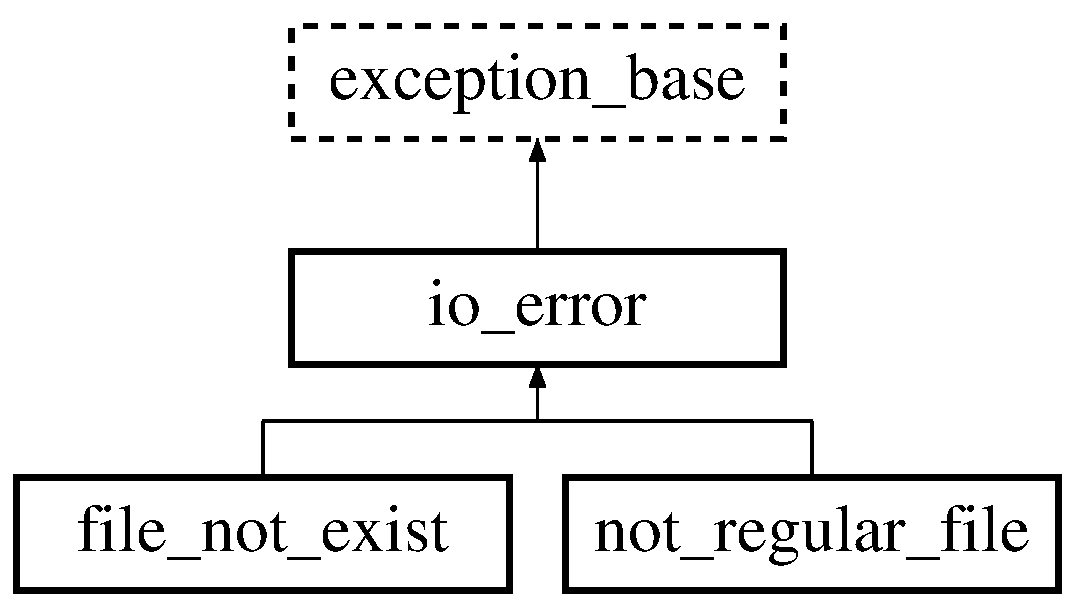
\includegraphics[height=3.000000cm]{structio__error}
\end{center}
\end{figure}


\subsection{\-Detailed \-Description}
struct defining the base of the \hyperlink{class_i_o}{\-I\-O} errors 

\-The documentation for this class was generated from the following file\-:\begin{DoxyCompactItemize}
\item 
headers/\hyperlink{_exceptions_8h}{\-Exceptions.\-h}\end{DoxyCompactItemize}

\hypertarget{class_main_window}{\section{\-Main\-Window \-Class \-Reference}
\label{class_main_window}\index{\-Main\-Window@{\-Main\-Window}}
}


\-Builds the main window of the program extends from \-Q\-Main\-Window.  




{\ttfamily \#include $<$\-Main\-Window.\-h$>$}

\subsection*{\-Public \-Slots}
\begin{DoxyCompactItemize}
\item 
\hyperlink{class_my_area}{\-My\-Area} $\ast$ \hyperlink{class_main_window_a3ecd23a0dc61406e34522af9aae150bb}{open\-Tab} ()
\begin{DoxyCompactList}\small\item\em open a new tab \end{DoxyCompactList}\item 
\hypertarget{class_main_window_a3ba1a371fb10e731ae0926ae85efeb4f}{void \hyperlink{class_main_window_a3ba1a371fb10e731ae0926ae85efeb4f}{save} ()}\label{class_main_window_a3ba1a371fb10e731ae0926ae85efeb4f}

\begin{DoxyCompactList}\small\item\em save the file \end{DoxyCompactList}\item 
\hypertarget{class_main_window_af622a541e4d87f86e9e83d29af60fe19}{void \hyperlink{class_main_window_af622a541e4d87f86e9e83d29af60fe19}{close\-Tab} ()}\label{class_main_window_af622a541e4d87f86e9e83d29af60fe19}

\begin{DoxyCompactList}\small\item\em close the active tab \end{DoxyCompactList}\item 
\hypertarget{class_main_window_a111875a1d82e77178636322ab485e4bb}{void \hyperlink{class_main_window_a111875a1d82e77178636322ab485e4bb}{export\-Png} ()}\label{class_main_window_a111875a1d82e77178636322ab485e4bb}

\begin{DoxyCompactList}\small\item\em export the actual view to \-P\-N\-G file \end{DoxyCompactList}\item 
\hypertarget{class_main_window_a879f655b0a921bc80bd316579e98c366}{void \hyperlink{class_main_window_a879f655b0a921bc80bd316579e98c366}{find\-Fixpoints} ()}\label{class_main_window_a879f655b0a921bc80bd316579e98c366}

\begin{DoxyCompactList}\small\item\em calls ph-\/stable functionality of pint \end{DoxyCompactList}\item 
\hypertarget{class_main_window_a0c7fe8e75bbc5113df5e514214908ab3}{void \hyperlink{class_main_window_a0c7fe8e75bbc5113df5e514214908ab3}{compute\-Reachability} ()}\label{class_main_window_a0c7fe8e75bbc5113df5e514214908ab3}

\begin{DoxyCompactList}\small\item\em calls ph-\/reach functionality of pint \end{DoxyCompactList}\item 
\hypertarget{class_main_window_ab8eeb1e902f4591fc2f35237a1faef01}{void \hyperlink{class_main_window_ab8eeb1e902f4591fc2f35237a1faef01}{run\-Stochastic\-Simulation} ()}\label{class_main_window_ab8eeb1e902f4591fc2f35237a1faef01}

\begin{DoxyCompactList}\small\item\em calls ph-\/exec functionality of pint \end{DoxyCompactList}\item 
\hypertarget{class_main_window_ace4bc6f63b25822514dd2250bbb4760f}{void \hyperlink{class_main_window_ace4bc6f63b25822514dd2250bbb4760f}{check\-Model\-Type} ()}\label{class_main_window_ace4bc6f63b25822514dd2250bbb4760f}

\begin{DoxyCompactList}\small\item\em checks the type of the model \end{DoxyCompactList}\item 
\hypertarget{class_main_window_a3eee76227ea883705553abe5e1f2a2be}{void \hyperlink{class_main_window_a3eee76227ea883705553abe5e1f2a2be}{statistics} ()}\label{class_main_window_a3eee76227ea883705553abe5e1f2a2be}

\begin{DoxyCompactList}\small\item\em calls ph-\/stat functionality of pint \end{DoxyCompactList}\item 
void \hyperlink{class_main_window_a5f56ea1ee38eb16074e654b8bd52d072}{disable\-Menu} (\-Q\-Mdi\-Sub\-Window $\ast$sub\-Window)
\begin{DoxyCompactList}\small\item\em permits to disable a menu \end{DoxyCompactList}\end{DoxyCompactItemize}
\subsection*{\-Public \-Member \-Functions}
\begin{DoxyCompactItemize}
\item 
\hypertarget{class_main_window_a34c4b4207b46d11a4100c9b19f0e81bb}{\hyperlink{class_main_window_a34c4b4207b46d11a4100c9b19f0e81bb}{\-Main\-Window} ()}\label{class_main_window_a34c4b4207b46d11a4100c9b19f0e81bb}

\begin{DoxyCompactList}\small\item\em builder for \hyperlink{class_main_window}{\-Main\-Window}, creates the window, the menus and initializes the characteristics \end{DoxyCompactList}\item 
\-Q\-Mdi\-Area $\ast$ \hyperlink{class_main_window_a398296c146bb239d0b75a24b44132658}{get\-Centrale\-Area} ()
\begin{DoxyCompactList}\small\item\em getter for \-Centrale\-Area \end{DoxyCompactList}\item 
\hypertarget{class_main_window_a5cc52553f615cb3abeb1198ad8c018a3}{std\-::vector$<$ \-Q\-String $>$ \hyperlink{class_main_window_a5cc52553f615cb3abeb1198ad8c018a3}{get\-All\-Paths} ()}\label{class_main_window_a5cc52553f615cb3abeb1198ad8c018a3}

\begin{DoxyCompactList}\small\item\em gets all the paths of the \hyperlink{class_p_h}{\-P\-H} files already opened \end{DoxyCompactList}\item 
void \hyperlink{class_main_window_a8a30572d7170d0a51737cd4991f0a05f}{compute} (\-Q\-String program, \-Q\-String\-List arguments, \-Q\-String file\-Name=\char`\"{}\char`\"{})
\begin{DoxyCompactList}\small\item\em calls the pint function with the arguments chosen \end{DoxyCompactList}\item 
\hypertarget{class_main_window_ac4c3ec77ba5666ff9ef670b4b02c6838}{void \hyperlink{class_main_window_ac4c3ec77ba5666ff9ef670b4b02c6838}{enable\-Menu} ()}\label{class_main_window_ac4c3ec77ba5666ff9ef670b4b02c6838}

\begin{DoxyCompactList}\small\item\em activates the menus that need a open an active tab \end{DoxyCompactList}\end{DoxyCompactItemize}
\subsection*{\-Protected \-Attributes}
\begin{DoxyCompactItemize}
\item 
\hypertarget{class_main_window_af5df9378db57a148236d639dd928d08f}{\-Q\-Mdi\-Area $\ast$ \hyperlink{class_main_window_af5df9378db57a148236d639dd928d08f}{centrale\-Area}}\label{class_main_window_af5df9378db57a148236d639dd928d08f}

\begin{DoxyCompactList}\small\item\em pointer to the centrale area of the window \end{DoxyCompactList}\item 
\hypertarget{class_main_window_a2ca04227e7d71b036ccd0ed4176a5561}{\-Q\-Menu $\ast$ {\bfseries menu\-File}}\label{class_main_window_a2ca04227e7d71b036ccd0ed4176a5561}

\item 
\hypertarget{class_main_window_a51ec7fcfcb60073b395dee46daacf1f9}{\-Q\-Menu $\ast$ {\bfseries menu\-Edit}}\label{class_main_window_a51ec7fcfcb60073b395dee46daacf1f9}

\item 
\hypertarget{class_main_window_a57793b17cc2b8de42b5b10e9458ae9cb}{\-Q\-Menu $\ast$ {\bfseries menu\-View}}\label{class_main_window_a57793b17cc2b8de42b5b10e9458ae9cb}

\item 
\hypertarget{class_main_window_a8142152915924723cee2f22e0868a852}{\-Q\-Menu $\ast$ {\bfseries menu\-Computation}}\label{class_main_window_a8142152915924723cee2f22e0868a852}

\item 
\hypertarget{class_main_window_a81d80bba8e8a31cea2bb218094890c81}{\-Q\-Menu $\ast$ {\bfseries menu\-Help}}\label{class_main_window_a81d80bba8e8a31cea2bb218094890c81}

\item 
\hypertarget{class_main_window_afcc4de380e40fe4aeb61b07402f00f58}{\-Q\-Action $\ast$ {\bfseries action\-New}}\label{class_main_window_afcc4de380e40fe4aeb61b07402f00f58}

\item 
\hypertarget{class_main_window_ab5342d85523e2dad5b6f69a6ad01ece3}{\-Q\-Action $\ast$ {\bfseries action\-Open}}\label{class_main_window_ab5342d85523e2dad5b6f69a6ad01ece3}

\item 
\hypertarget{class_main_window_ac785bdaae348156fc94fdfea23f67a90}{\-Q\-Action $\ast$ {\bfseries action\-Saveas}}\label{class_main_window_ac785bdaae348156fc94fdfea23f67a90}

\item 
\hypertarget{class_main_window_a509ebce4344493751dec180d55d3b107}{\-Q\-Menu $\ast$ {\bfseries menu\-Export}}\label{class_main_window_a509ebce4344493751dec180d55d3b107}

\item 
\hypertarget{class_main_window_a233dc8b191a12c682366d27a3d9e568f}{\-Q\-Action $\ast$ {\bfseries action\-Png}}\label{class_main_window_a233dc8b191a12c682366d27a3d9e568f}

\item 
\hypertarget{class_main_window_acf4206ba3c373585ad33ef09e0c8ccb3}{\-Q\-Action $\ast$ {\bfseries action\-Close}}\label{class_main_window_acf4206ba3c373585ad33ef09e0c8ccb3}

\item 
\hypertarget{class_main_window_a60f400ff0f2b281499611c5e0018d901}{\-Q\-Action $\ast$ {\bfseries action\-Quit}}\label{class_main_window_a60f400ff0f2b281499611c5e0018d901}

\item 
\hypertarget{class_main_window_aca6e412c6008053d39c5fbaf5133274b}{\-Q\-Action $\ast$ {\bfseries action\-Undo}}\label{class_main_window_aca6e412c6008053d39c5fbaf5133274b}

\item 
\hypertarget{class_main_window_aa1ea7fe519e373af34ba4f7669df14cd}{\-Q\-Action $\ast$ {\bfseries action\-Redo}}\label{class_main_window_aa1ea7fe519e373af34ba4f7669df14cd}

\item 
\hypertarget{class_main_window_a1149df8ffebf08ca08bafcef304a207a}{\-Q\-Action $\ast$ {\bfseries action\-Show\-Init}}\label{class_main_window_a1149df8ffebf08ca08bafcef304a207a}

\item 
\hypertarget{class_main_window_aab91a08cf5e63146ac25d266699344f7}{\-Q\-Action $\ast$ {\bfseries action\-Highlight}}\label{class_main_window_aab91a08cf5e63146ac25d266699344f7}

\item 
\hypertarget{class_main_window_a8d65feefc7d6d3d809b2466be1b6c176}{\-Q\-Action $\ast$ {\bfseries action\-Hide}}\label{class_main_window_a8d65feefc7d6d3d809b2466be1b6c176}

\item 
\hypertarget{class_main_window_afea5009cf5a1589c7921992310620c3f}{\-Q\-Action $\ast$ {\bfseries action\-Display\-Detailed}}\label{class_main_window_afea5009cf5a1589c7921992310620c3f}

\item 
\hypertarget{class_main_window_a04048deb025090490f7261002a4ea4ab}{\-Q\-Action $\ast$ {\bfseries action\-Find\-Fixpoints}}\label{class_main_window_a04048deb025090490f7261002a4ea4ab}

\item 
\hypertarget{class_main_window_a2d5f7f2433aab9c8005c197bc96cdbc9}{\-Q\-Action $\ast$ {\bfseries action\-Compute\-Reachability}}\label{class_main_window_a2d5f7f2433aab9c8005c197bc96cdbc9}

\item 
\hypertarget{class_main_window_ae1ed3e80e7e9dc6e0687729e68071c37}{\-Q\-Action $\ast$ {\bfseries action\-Run\-Stochastic\-Simulation}}\label{class_main_window_ae1ed3e80e7e9dc6e0687729e68071c37}

\item 
\hypertarget{class_main_window_ab44ca117cab372eb7baea30cf0a6c8b0}{\-Q\-Action $\ast$ {\bfseries action\-Check\-Model\-Type}}\label{class_main_window_ab44ca117cab372eb7baea30cf0a6c8b0}

\item 
\hypertarget{class_main_window_ab81ef1d7f2f2dfc26b8ca9b50391692d}{\-Q\-Action $\ast$ {\bfseries action\-Statistics}}\label{class_main_window_ab81ef1d7f2f2dfc26b8ca9b50391692d}

\item 
\hypertarget{class_main_window_aa533eee89cb4ec348b3df9c25f10f47f}{\-Q\-Action $\ast$ {\bfseries action\-Help}}\label{class_main_window_aa533eee89cb4ec348b3df9c25f10f47f}

\end{DoxyCompactItemize}


\subsection{\-Detailed \-Description}
\-Builds the main window of the program extends from \-Q\-Main\-Window. 

\subsection{\-Member \-Function \-Documentation}
\hypertarget{class_main_window_a8a30572d7170d0a51737cd4991f0a05f}{\index{\-Main\-Window@{\-Main\-Window}!compute@{compute}}
\index{compute@{compute}!MainWindow@{\-Main\-Window}}
\subsubsection[{compute}]{\setlength{\rightskip}{0pt plus 5cm}void {\bf \-Main\-Window\-::compute} (
\begin{DoxyParamCaption}
\item[{\-Q\-String}]{program, }
\item[{\-Q\-String\-List}]{arguments, }
\item[{\-Q\-String}]{file\-Name = {\ttfamily \char`\"{}\char`\"{}}}
\end{DoxyParamCaption}
)}}\label{class_main_window_a8a30572d7170d0a51737cd4991f0a05f}


calls the pint function with the arguments chosen 


\begin{DoxyParams}{\-Parameters}
{\em \-Qstring} & the program chosen \\
\hline
{\em \-Q\-String\-List} & the arguments chosen \\
\hline
{\em \-Q\-String} & the name of the file (optionnal) \\
\hline
\end{DoxyParams}
\hypertarget{class_main_window_a5f56ea1ee38eb16074e654b8bd52d072}{\index{\-Main\-Window@{\-Main\-Window}!disable\-Menu@{disable\-Menu}}
\index{disable\-Menu@{disable\-Menu}!MainWindow@{\-Main\-Window}}
\subsubsection[{disable\-Menu}]{\setlength{\rightskip}{0pt plus 5cm}void {\bf \-Main\-Window\-::disable\-Menu} (
\begin{DoxyParamCaption}
\item[{\-Q\-Mdi\-Sub\-Window $\ast$}]{sub\-Window}
\end{DoxyParamCaption}
)\hspace{0.3cm}{\ttfamily  \mbox{[}slot\mbox{]}}}}\label{class_main_window_a5f56ea1ee38eb16074e654b8bd52d072}


permits to disable a menu 


\begin{DoxyParams}{\-Parameters}
{\em \-Q\-Mdi\-Sub\-Window$\ast$} & menu you want to disable \\
\hline
\end{DoxyParams}
\hypertarget{class_main_window_a398296c146bb239d0b75a24b44132658}{\index{\-Main\-Window@{\-Main\-Window}!get\-Centrale\-Area@{get\-Centrale\-Area}}
\index{get\-Centrale\-Area@{get\-Centrale\-Area}!MainWindow@{\-Main\-Window}}
\subsubsection[{get\-Centrale\-Area}]{\setlength{\rightskip}{0pt plus 5cm}\-Q\-Mdi\-Area$\ast$ {\bf \-Main\-Window\-::get\-Centrale\-Area} (
\begin{DoxyParamCaption}
{}
\end{DoxyParamCaption}
)}}\label{class_main_window_a398296c146bb239d0b75a24b44132658}


getter for \-Centrale\-Area 

\begin{DoxyReturn}{\-Returns}
a \-Q\-Mdi\-Area$\ast$ pointer to the centrale zone of the window 
\end{DoxyReturn}
\hypertarget{class_main_window_a3ecd23a0dc61406e34522af9aae150bb}{\index{\-Main\-Window@{\-Main\-Window}!open\-Tab@{open\-Tab}}
\index{open\-Tab@{open\-Tab}!MainWindow@{\-Main\-Window}}
\subsubsection[{open\-Tab}]{\setlength{\rightskip}{0pt plus 5cm}{\bf \-My\-Area}$\ast$ {\bf \-Main\-Window\-::open\-Tab} (
\begin{DoxyParamCaption}
{}
\end{DoxyParamCaption}
)\hspace{0.3cm}{\ttfamily  \mbox{[}slot\mbox{]}}}}\label{class_main_window_a3ecd23a0dc61406e34522af9aae150bb}


open a new tab 

\begin{DoxyReturn}{\-Returns}
a pointer to a \hyperlink{class_my_area}{\-My\-Area} newly created 
\end{DoxyReturn}


\-The documentation for this class was generated from the following file\-:\begin{DoxyCompactItemize}
\item 
headers/\hyperlink{_main_window_8h}{\-Main\-Window.\-h}\end{DoxyCompactItemize}

\hypertarget{class_my_area}{\section{\-My\-Area \-Class \-Reference}
\label{class_my_area}\index{\-My\-Area@{\-My\-Area}}
}


new tab extends \-Q\-Graphics\-View  




{\ttfamily \#include $<$\-My\-Area.\-h$>$}

\subsection*{\-Public \-Member \-Functions}
\begin{DoxyCompactItemize}
\item 
\hypertarget{class_my_area_a31f13e95c83414c538b6c46e55e19c79}{\hyperlink{class_my_area_a31f13e95c83414c538b6c46e55e19c79}{\-My\-Area} (\-Q\-String \hyperlink{class_my_area_a70561a408470de740f580da6717871bf}{path})}\label{class_my_area_a31f13e95c83414c538b6c46e55e19c79}

\begin{DoxyCompactList}\small\item\em builder for \hyperlink{class_my_area}{\-My\-Area} param path of the area \end{DoxyCompactList}\item 
\hypertarget{class_my_area_a7b94b516e730ddcee16d946c76bbc2b3}{\-P\-H\-Ptr \hyperlink{class_my_area_a7b94b516e730ddcee16d946c76bbc2b3}{get\-P\-H\-Ptr} ()}\label{class_my_area_a7b94b516e730ddcee16d946c76bbc2b3}

\begin{DoxyCompactList}\small\item\em getter for my\-P\-H\-Ptr \end{DoxyCompactList}\item 
\hypertarget{class_my_area_a087c389370070a348af025aaee620fc8}{void \hyperlink{class_my_area_a087c389370070a348af025aaee620fc8}{set\-P\-H\-Ptr} (\-P\-H\-Ptr)}\label{class_my_area_a087c389370070a348af025aaee620fc8}

\begin{DoxyCompactList}\small\item\em setter for my\-P\-H\-Ptr \end{DoxyCompactList}\item 
\hypertarget{class_my_area_a84edb9791a8c988cb9f13ac1ef2025d5}{\-Q\-String \hyperlink{class_my_area_a84edb9791a8c988cb9f13ac1ef2025d5}{get\-Path} ()}\label{class_my_area_a84edb9791a8c988cb9f13ac1ef2025d5}

\begin{DoxyCompactList}\small\item\em getter for the path \end{DoxyCompactList}\item 
\hypertarget{class_my_area_ab1f574dcb5318131128deb076743f01a}{void \hyperlink{class_my_area_ab1f574dcb5318131128deb076743f01a}{set\-Path} (\-Q\-String)}\label{class_my_area_ab1f574dcb5318131128deb076743f01a}

\begin{DoxyCompactList}\small\item\em setter for the path \end{DoxyCompactList}\end{DoxyCompactItemize}
\subsection*{\-Protected \-Attributes}
\begin{DoxyCompactItemize}
\item 
\hypertarget{class_my_area_a59beb02fefc60d81c287cbc43e6de640}{\-P\-H\-Ptr \hyperlink{class_my_area_a59beb02fefc60d81c287cbc43e6de640}{my\-P\-H\-Ptr}}\label{class_my_area_a59beb02fefc60d81c287cbc43e6de640}

\begin{DoxyCompactList}\small\item\em pointer to a \hyperlink{class_p_h}{\-P\-H} object \end{DoxyCompactList}\item 
\hypertarget{class_my_area_a70561a408470de740f580da6717871bf}{\-Q\-String \hyperlink{class_my_area_a70561a408470de740f580da6717871bf}{path}}\label{class_my_area_a70561a408470de740f580da6717871bf}

\begin{DoxyCompactList}\small\item\em contains the path to the file \end{DoxyCompactList}\end{DoxyCompactItemize}


\subsection{\-Detailed \-Description}
new tab extends \-Q\-Graphics\-View 

\-The documentation for this class was generated from the following file\-:\begin{DoxyCompactItemize}
\item 
headers/\hyperlink{_my_area_8h}{\-My\-Area.\-h}\end{DoxyCompactItemize}

\hypertarget{structnot__regular__file}{\section{not\-\_\-regular\-\_\-file \-Class \-Reference}
\label{structnot__regular__file}\index{not\-\_\-regular\-\_\-file@{not\-\_\-regular\-\_\-file}}
}


struct defining the exception called when the format of the file is not the one expected extends \hyperlink{structio__error}{io\-\_\-error}  




{\ttfamily \#include $<$\-Exceptions.\-h$>$}

\-Inheritance diagram for not\-\_\-regular\-\_\-file\-:\begin{figure}[H]
\begin{center}
\leavevmode
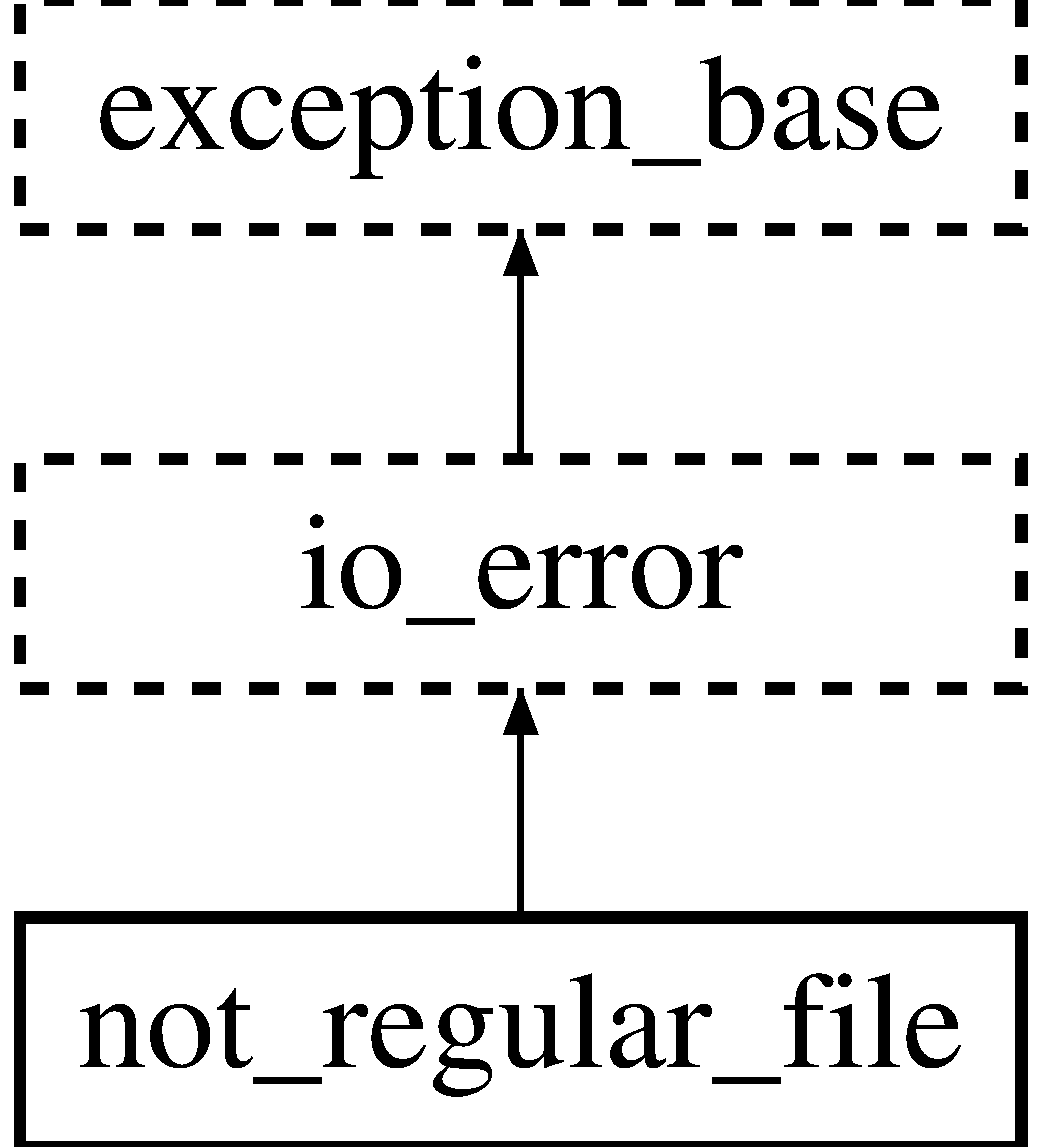
\includegraphics[height=3.000000cm]{structnot__regular__file}
\end{center}
\end{figure}


\subsection{\-Detailed \-Description}
struct defining the exception called when the format of the file is not the one expected extends \hyperlink{structio__error}{io\-\_\-error} 

\-The documentation for this class was generated from the following file\-:\begin{DoxyCompactItemize}
\item 
headers/\hyperlink{_exceptions_8h}{\-Exceptions.\-h}\end{DoxyCompactItemize}

\hypertarget{class_p_h}{\section{\-P\-H \-Class \-Reference}
\label{class_p_h}\index{\-P\-H@{\-P\-H}}
}


represents an entire process hitting as defined in a \hyperlink{class_p_h}{\-P\-H} file  




{\ttfamily \#include $<$\-P\-H.\-h$>$}

\subsection*{\-Public \-Member \-Functions}
\begin{DoxyCompactItemize}
\item 
\hypertarget{class_p_h_ae3ab2dd87b4bfadf04c1a14c6091aebc}{\hyperlink{class_p_h_ae3ab2dd87b4bfadf04c1a14c6091aebc}{\-P\-H} ()}\label{class_p_h_ae3ab2dd87b4bfadf04c1a14c6091aebc}

\begin{DoxyCompactList}\small\item\em constructor \end{DoxyCompactList}\item 
void \hyperlink{class_p_h_ad4335e01899c57e6802021f1afb83e7f}{add\-Sort} (\-Sort\-Ptr s)
\begin{DoxyCompactList}\small\item\em adds a sort to the \hyperlink{class_p_h}{\-P\-H} \end{DoxyCompactList}\item 
void \hyperlink{class_p_h_ae9bed9356d272f3c43f2147d6d8e5906}{add\-Action} (\-Action\-Ptr a)
\begin{DoxyCompactList}\small\item\em adds an action to the \hyperlink{class_p_h}{\-P\-H} \end{DoxyCompactList}\item 
\hypertarget{class_p_h_a02f1cd90c270555a50c08caa0fb2d491}{\-Sort\-Ptr \hyperlink{class_p_h_a02f1cd90c270555a50c08caa0fb2d491}{get\-Sort} (string const \&)}\label{class_p_h_a02f1cd90c270555a50c08caa0fb2d491}

\begin{DoxyCompactList}\small\item\em getter for a sort \end{DoxyCompactList}\item 
\hypertarget{class_p_h_ae9861660fe017ab285451b2ac8e191a4}{list$<$ \-Action\-Ptr $>$ \hyperlink{class_p_h_ae9861660fe017ab285451b2ac8e191a4}{get\-Actions} (void)}\label{class_p_h_ae9861660fe017ab285451b2ac8e191a4}

\begin{DoxyCompactList}\small\item\em getter for the actions of the \hyperlink{class_p_h}{\-P\-H} \end{DoxyCompactList}\item 
\hypertarget{class_p_h_a12e6b41c19521b568df7f86e6979167a}{list$<$ \-Sort\-Ptr $>$ \hyperlink{class_p_h_a12e6b41c19521b568df7f86e6979167a}{get\-Sorts} (void)}\label{class_p_h_a12e6b41c19521b568df7f86e6979167a}

\begin{DoxyCompactList}\small\item\em getter for the sorts of the \hyperlink{class_p_h}{\-P\-H} \end{DoxyCompactList}\item 
\hypertarget{class_p_h_a0155be0ca23e141f4c463f7b6a59051f}{list$<$ \-Process\-Ptr $>$ \hyperlink{class_p_h_a0155be0ca23e141f4c463f7b6a59051f}{get\-Processes} (void)}\label{class_p_h_a0155be0ca23e141f4c463f7b6a59051f}

\begin{DoxyCompactList}\small\item\em getter for the processes of the \hyperlink{class_p_h}{\-P\-H} \end{DoxyCompactList}\item 
string \hyperlink{class_p_h_ae870206aad796943dffaa6bab1f7f293}{to\-String} (void)
\begin{DoxyCompactList}\small\item\em gives a text representation of the process hitting (as it would be in a .ph file) \end{DoxyCompactList}\item 
string \hyperlink{class_p_h_aa0a7716cb565380f06670517609ee960}{to\-Dot\-String} (void)
\begin{DoxyCompactList}\small\item\em gives a text representation of the process hitting (in .dot format, used in \-Graphviz) \end{DoxyCompactList}\item 
void \hyperlink{class_p_h_af1f67304076aded44a15a30aed6dc652}{render} (void)
\begin{DoxyCompactList}\small\item\em calls for the process hitting in its scene \end{DoxyCompactList}\item 
\-G\-V\-Graph\-Ptr \hyperlink{class_p_h_a220fd9fdc673988edb461b02a90edb1b}{to\-G\-V\-Graph} (void)
\begin{DoxyCompactList}\small\item\em makes a representation of the process hitting as a graph \end{DoxyCompactList}\item 
\-G\-V\-Graph\-Ptr \hyperlink{class_p_h_afbd5cbabc39a0502a95e5c6609a52d58}{update\-G\-V\-Graph} (\hyperlink{class_p_h_scene}{\-P\-H\-Scene} $\ast$\hyperlink{class_p_h_ac8fbe29746ee4097c879be0cf75f3ad7}{scene})
\begin{DoxyCompactList}\small\item\em updates the representation of the process hitting as a graph after user's customizations \end{DoxyCompactList}\item 
\-P\-H\-Scene\-Ptr \hyperlink{class_p_h_aaf75a785bb9bd06cec611f0fb69d05f6}{get\-Graphics\-Scene} (void)
\begin{DoxyCompactList}\small\item\em outputs for display \end{DoxyCompactList}\item 
\hypertarget{class_p_h_a0494ca8a53e983230a9df06fa71043e1}{int \hyperlink{class_p_h_a0494ca8a53e983230a9df06fa71043e1}{get\-Stochasticity\-Absorption} ()}\label{class_p_h_a0494ca8a53e983230a9df06fa71043e1}

\begin{DoxyCompactList}\small\item\em getter for the stochasticity absorption \end{DoxyCompactList}\item 
\hypertarget{class_p_h_a78fb558177760ed0e640d8a0aaf8b06a}{void \hyperlink{class_p_h_a78fb558177760ed0e640d8a0aaf8b06a}{set\-Stochasticity\-Absorption} (int sa)}\label{class_p_h_a78fb558177760ed0e640d8a0aaf8b06a}

\begin{DoxyCompactList}\small\item\em setter for the stochasticity absorption \end{DoxyCompactList}\item 
\hypertarget{class_p_h_aa64e3d43f773122df2329491f6abdf6c}{double \hyperlink{class_p_h_aa64e3d43f773122df2329491f6abdf6c}{get\-Default\-Rate} ()}\label{class_p_h_aa64e3d43f773122df2329491f6abdf6c}

\begin{DoxyCompactList}\small\item\em getter for the default rate; \end{DoxyCompactList}\item 
\hypertarget{class_p_h_ae49be2823d5a2a7c6517b6783cf9fdfa}{void \hyperlink{class_p_h_ae49be2823d5a2a7c6517b6783cf9fdfa}{set\-Default\-Rate} (double r)}\label{class_p_h_ae49be2823d5a2a7c6517b6783cf9fdfa}

\begin{DoxyCompactList}\small\item\em setter for the default rate \end{DoxyCompactList}\item 
\hypertarget{class_p_h_a7ede855d04ee8e3a20beb159c5520003}{bool \hyperlink{class_p_h_a7ede855d04ee8e3a20beb159c5520003}{get\-Infinite\-Default\-Rate} ()}\label{class_p_h_a7ede855d04ee8e3a20beb159c5520003}

\begin{DoxyCompactList}\small\item\em getter for the \-Infinite \-Default \-Rate \end{DoxyCompactList}\item 
\hypertarget{class_p_h_acc38a15dc0e29ddfd2c8ae7d3371f7ab}{void \hyperlink{class_p_h_acc38a15dc0e29ddfd2c8ae7d3371f7ab}{set\-Infinite\-Default\-Rate} (bool b)}\label{class_p_h_acc38a15dc0e29ddfd2c8ae7d3371f7ab}

\begin{DoxyCompactList}\small\item\em setter for the \-Infinitite \-Default \-Rate \end{DoxyCompactList}\end{DoxyCompactItemize}
\subsection*{\-Protected \-Attributes}
\begin{DoxyCompactItemize}
\item 
\hypertarget{class_p_h_abdd55c7db00c19b89de0afba20d97b24}{int \hyperlink{class_p_h_abdd55c7db00c19b89de0afba20d97b24}{stochasticity\-\_\-absorption}}\label{class_p_h_abdd55c7db00c19b89de0afba20d97b24}

\begin{DoxyCompactList}\small\item\em default value for stochasticity absorption \end{DoxyCompactList}\item 
bool \hyperlink{class_p_h_aa66efaf095a379c3b108a023d7c98afa}{infinite\-\_\-default\-\_\-rate}
\begin{DoxyCompactList}\small\item\em boolean to know if the default rate is or is not infinite \end{DoxyCompactList}\item 
\hypertarget{class_p_h_a7a9525bc83257efefbaf9e78d96723ca}{double \hyperlink{class_p_h_a7a9525bc83257efefbaf9e78d96723ca}{default\-\_\-rate}}\label{class_p_h_a7a9525bc83257efefbaf9e78d96723ca}

\begin{DoxyCompactList}\small\item\em default value for rate \end{DoxyCompactList}\item 
\hypertarget{class_p_h_a889cc129633e88e4257f56dec04c5bac}{map$<$ string, \-Sort\-Ptr $>$ \hyperlink{class_p_h_a889cc129633e88e4257f56dec04c5bac}{sorts}}\label{class_p_h_a889cc129633e88e4257f56dec04c5bac}

\begin{DoxyCompactList}\small\item\em map of the sorts, linked with their names \end{DoxyCompactList}\item 
\hypertarget{class_p_h_a730f2eb0cd79487213cac9565d746a05}{list$<$ \-Action\-Ptr $>$ \hyperlink{class_p_h_a730f2eb0cd79487213cac9565d746a05}{actions}}\label{class_p_h_a730f2eb0cd79487213cac9565d746a05}

\begin{DoxyCompactList}\small\item\em list of the actions \end{DoxyCompactList}\item 
\hypertarget{class_p_h_ac8fbe29746ee4097c879be0cf75f3ad7}{\-P\-H\-Scene\-Ptr \hyperlink{class_p_h_ac8fbe29746ee4097c879be0cf75f3ad7}{scene}}\label{class_p_h_ac8fbe29746ee4097c879be0cf75f3ad7}

\begin{DoxyCompactList}\small\item\em graphical object representing the process hitting \end{DoxyCompactList}\end{DoxyCompactItemize}


\subsection{\-Detailed \-Description}
represents an entire process hitting as defined in a \hyperlink{class_p_h}{\-P\-H} file 

\subsection{\-Member \-Function \-Documentation}
\hypertarget{class_p_h_ae9bed9356d272f3c43f2147d6d8e5906}{\index{\-P\-H@{\-P\-H}!add\-Action@{add\-Action}}
\index{add\-Action@{add\-Action}!PH@{\-P\-H}}
\subsubsection[{add\-Action}]{\setlength{\rightskip}{0pt plus 5cm}void {\bf \-P\-H\-::add\-Action} (
\begin{DoxyParamCaption}
\item[{\-Action\-Ptr}]{a}
\end{DoxyParamCaption}
)}}\label{class_p_h_ae9bed9356d272f3c43f2147d6d8e5906}


adds an action to the \hyperlink{class_p_h}{\-P\-H} 


\begin{DoxyParams}{\-Parameters}
{\em \-Action\-Ptr} & the action to add \\
\hline
\end{DoxyParams}
\hypertarget{class_p_h_ad4335e01899c57e6802021f1afb83e7f}{\index{\-P\-H@{\-P\-H}!add\-Sort@{add\-Sort}}
\index{add\-Sort@{add\-Sort}!PH@{\-P\-H}}
\subsubsection[{add\-Sort}]{\setlength{\rightskip}{0pt plus 5cm}void {\bf \-P\-H\-::add\-Sort} (
\begin{DoxyParamCaption}
\item[{\-Sort\-Ptr}]{s}
\end{DoxyParamCaption}
)}}\label{class_p_h_ad4335e01899c57e6802021f1afb83e7f}


adds a sort to the \hyperlink{class_p_h}{\-P\-H} 


\begin{DoxyParams}{\-Parameters}
{\em \-Sort\-Ptr} & the sort to add \\
\hline
\end{DoxyParams}
\hypertarget{class_p_h_aaf75a785bb9bd06cec611f0fb69d05f6}{\index{\-P\-H@{\-P\-H}!get\-Graphics\-Scene@{get\-Graphics\-Scene}}
\index{get\-Graphics\-Scene@{get\-Graphics\-Scene}!PH@{\-P\-H}}
\subsubsection[{get\-Graphics\-Scene}]{\setlength{\rightskip}{0pt plus 5cm}\-P\-H\-Scene\-Ptr {\bf \-P\-H\-::get\-Graphics\-Scene} (
\begin{DoxyParamCaption}
\item[{void}]{}
\end{DoxyParamCaption}
)}}\label{class_p_h_aaf75a785bb9bd06cec611f0fb69d05f6}


outputs for display 

\begin{DoxyReturn}{\-Returns}
\-P\-H\-Scene\-Ptr pointer to the \-Scene built 
\end{DoxyReturn}
\hypertarget{class_p_h_af1f67304076aded44a15a30aed6dc652}{\index{\-P\-H@{\-P\-H}!render@{render}}
\index{render@{render}!PH@{\-P\-H}}
\subsubsection[{render}]{\setlength{\rightskip}{0pt plus 5cm}void {\bf \-P\-H\-::render} (
\begin{DoxyParamCaption}
\item[{void}]{}
\end{DoxyParamCaption}
)}}\label{class_p_h_af1f67304076aded44a15a30aed6dc652}


calls for the process hitting in its scene 

time-\/expensive method, calls the to\-G\-V\-Graph method \hypertarget{class_p_h_aa0a7716cb565380f06670517609ee960}{\index{\-P\-H@{\-P\-H}!to\-Dot\-String@{to\-Dot\-String}}
\index{to\-Dot\-String@{to\-Dot\-String}!PH@{\-P\-H}}
\subsubsection[{to\-Dot\-String}]{\setlength{\rightskip}{0pt plus 5cm}string {\bf \-P\-H\-::to\-Dot\-String} (
\begin{DoxyParamCaption}
\item[{void}]{}
\end{DoxyParamCaption}
)}}\label{class_p_h_aa0a7716cb565380f06670517609ee960}


gives a text representation of the process hitting (in .dot format, used in \-Graphviz) 

\begin{DoxyReturn}{\-Returns}
string the text representation of the process hitting in \-D\-O\-T format 
\end{DoxyReturn}
\hypertarget{class_p_h_a220fd9fdc673988edb461b02a90edb1b}{\index{\-P\-H@{\-P\-H}!to\-G\-V\-Graph@{to\-G\-V\-Graph}}
\index{to\-G\-V\-Graph@{to\-G\-V\-Graph}!PH@{\-P\-H}}
\subsubsection[{to\-G\-V\-Graph}]{\setlength{\rightskip}{0pt plus 5cm}\-G\-V\-Graph\-Ptr {\bf \-P\-H\-::to\-G\-V\-Graph} (
\begin{DoxyParamCaption}
\item[{void}]{}
\end{DoxyParamCaption}
)}}\label{class_p_h_a220fd9fdc673988edb461b02a90edb1b}


makes a representation of the process hitting as a graph 

calls graphviz to calculate the optimized graph \begin{DoxyReturn}{\-Returns}
\-G\-V\-Graph\-Ptr pointer to the \-Graph built 
\end{DoxyReturn}
\hypertarget{class_p_h_ae870206aad796943dffaa6bab1f7f293}{\index{\-P\-H@{\-P\-H}!to\-String@{to\-String}}
\index{to\-String@{to\-String}!PH@{\-P\-H}}
\subsubsection[{to\-String}]{\setlength{\rightskip}{0pt plus 5cm}string {\bf \-P\-H\-::to\-String} (
\begin{DoxyParamCaption}
\item[{void}]{}
\end{DoxyParamCaption}
)}}\label{class_p_h_ae870206aad796943dffaa6bab1f7f293}


gives a text representation of the process hitting (as it would be in a .ph file) 

\begin{DoxyReturn}{\-Returns}
string the text representation of the process hitting in \hyperlink{class_p_h}{\-P\-H} format 
\end{DoxyReturn}
\hypertarget{class_p_h_afbd5cbabc39a0502a95e5c6609a52d58}{\index{\-P\-H@{\-P\-H}!update\-G\-V\-Graph@{update\-G\-V\-Graph}}
\index{update\-G\-V\-Graph@{update\-G\-V\-Graph}!PH@{\-P\-H}}
\subsubsection[{update\-G\-V\-Graph}]{\setlength{\rightskip}{0pt plus 5cm}\-G\-V\-Graph\-Ptr {\bf \-P\-H\-::update\-G\-V\-Graph} (
\begin{DoxyParamCaption}
\item[{{\bf \-P\-H\-Scene} $\ast$}]{scene}
\end{DoxyParamCaption}
)}}\label{class_p_h_afbd5cbabc39a0502a95e5c6609a52d58}


updates the representation of the process hitting as a graph after user's customizations 

calls graphviz to calculate the graph \begin{DoxyReturn}{\-Returns}

\end{DoxyReturn}


\subsection{\-Member \-Data \-Documentation}
\hypertarget{class_p_h_aa66efaf095a379c3b108a023d7c98afa}{\index{\-P\-H@{\-P\-H}!infinite\-\_\-default\-\_\-rate@{infinite\-\_\-default\-\_\-rate}}
\index{infinite\-\_\-default\-\_\-rate@{infinite\-\_\-default\-\_\-rate}!PH@{\-P\-H}}
\subsubsection[{infinite\-\_\-default\-\_\-rate}]{\setlength{\rightskip}{0pt plus 5cm}bool {\bf \-P\-H\-::infinite\-\_\-default\-\_\-rate}\hspace{0.3cm}{\ttfamily  \mbox{[}protected\mbox{]}}}}\label{class_p_h_aa66efaf095a379c3b108a023d7c98afa}


boolean to know if the default rate is or is not infinite 

if true then the value of default rate makes no sense 

\-The documentation for this class was generated from the following file\-:\begin{DoxyCompactItemize}
\item 
headers/\hyperlink{_p_h_8h}{\-P\-H.\-h}\end{DoxyCompactItemize}

\hypertarget{structph__error}{\section{ph\-\_\-error \-Class \-Reference}
\label{structph__error}\index{ph\-\_\-error@{ph\-\_\-error}}
}


struct defining the exception called when there is an error in the \hyperlink{class_p_h}{\-P\-H} file extends \hyperlink{structexception__base}{exception\-\_\-base}  




{\ttfamily \#include $<$\-Exceptions.\-h$>$}

\-Inheritance diagram for ph\-\_\-error\-:\begin{figure}[H]
\begin{center}
\leavevmode
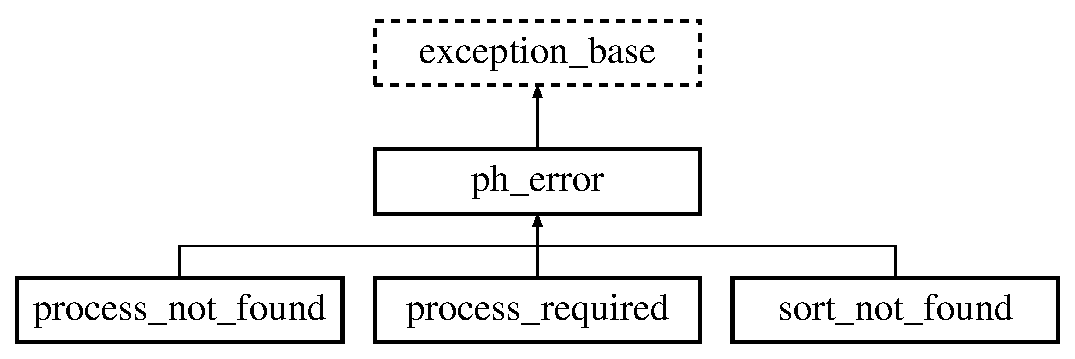
\includegraphics[height=3.000000cm]{structph__error}
\end{center}
\end{figure}


\subsection{\-Detailed \-Description}
struct defining the exception called when there is an error in the \hyperlink{class_p_h}{\-P\-H} file extends \hyperlink{structexception__base}{exception\-\_\-base} 

\-The documentation for this class was generated from the following file\-:\begin{DoxyCompactItemize}
\item 
headers/\hyperlink{_exceptions_8h}{\-Exceptions.\-h}\end{DoxyCompactItemize}

\hypertarget{structph__parse__error}{\section{ph\-\_\-parse\-\_\-error \-Class \-Reference}
\label{structph__parse__error}\index{ph\-\_\-parse\-\_\-error@{ph\-\_\-parse\-\_\-error}}
}


struct defining the exception called when the \hyperlink{class_p_h}{\-P\-H} file cannot be parsed extends \hyperlink{structexception__base}{exception\-\_\-base}  




{\ttfamily \#include $<$\-Exceptions.\-h$>$}

\-Inheritance diagram for ph\-\_\-parse\-\_\-error\-:\begin{figure}[H]
\begin{center}
\leavevmode
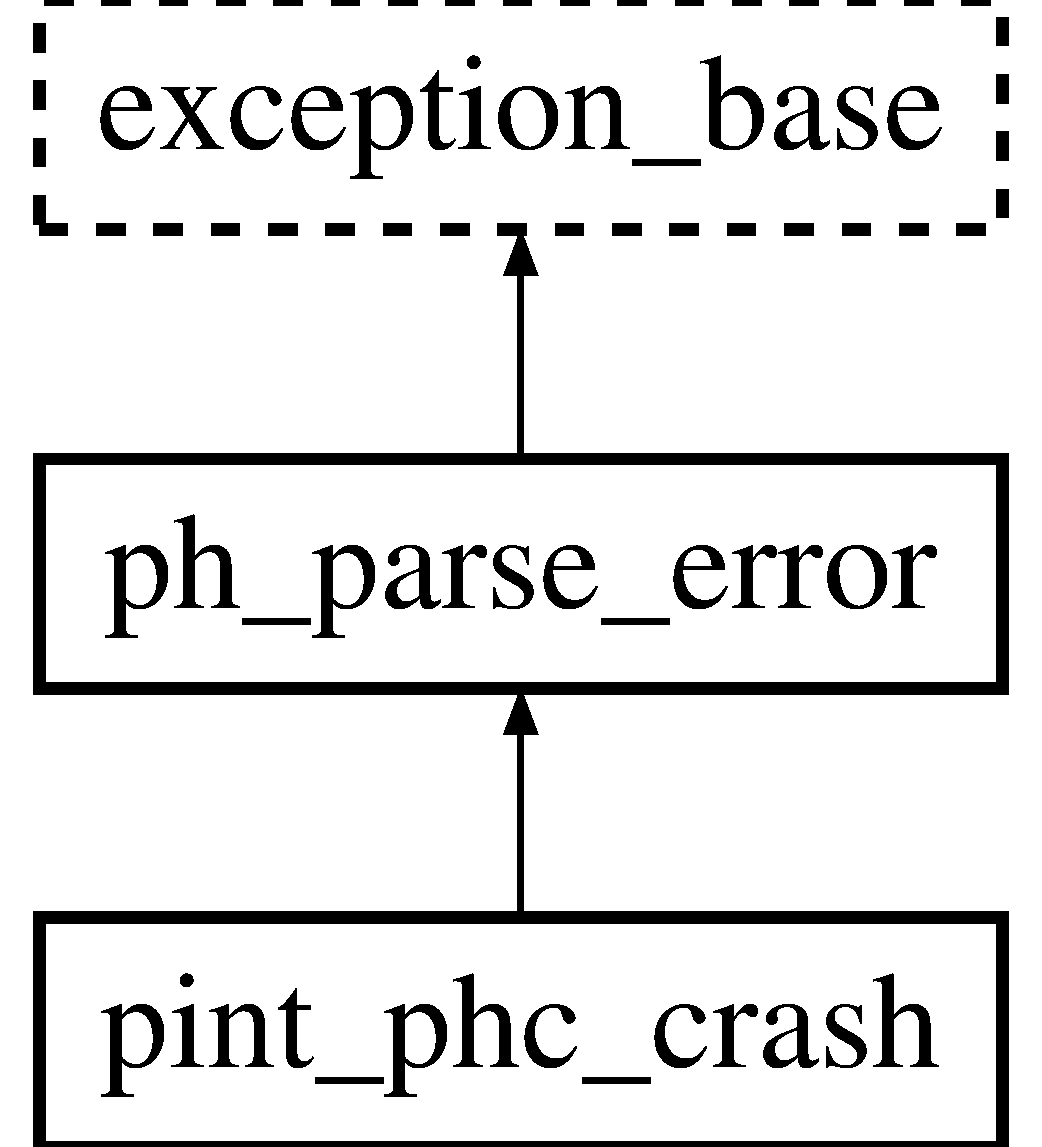
\includegraphics[height=3.000000cm]{structph__parse__error}
\end{center}
\end{figure}


\subsection{\-Detailed \-Description}
struct defining the exception called when the \hyperlink{class_p_h}{\-P\-H} file cannot be parsed extends \hyperlink{structexception__base}{exception\-\_\-base} 

\-The documentation for this class was generated from the following file\-:\begin{DoxyCompactItemize}
\item 
headers/\hyperlink{_exceptions_8h}{\-Exceptions.\-h}\end{DoxyCompactItemize}

\hypertarget{class_p_h_i_o}{\section{\-P\-H\-I\-O \-Class \-Reference}
\label{class_p_h_i_o}\index{\-P\-H\-I\-O@{\-P\-H\-I\-O}}
}


manages the inputs and outputs of the \hyperlink{class_p_h}{\-P\-H} files  




{\ttfamily \#include $<$\-P\-H\-I\-O.\-h$>$}

\subsection*{\-Static \-Public \-Member \-Functions}
\begin{DoxyCompactItemize}
\item 
static bool \hyperlink{class_p_h_i_o_a264cd5b35169906843e829a13cbcc09d}{can\-Parse\-File} (string const \&path)
\begin{DoxyCompactList}\small\item\em checks if the file exists and is recognized by the parser \end{DoxyCompactList}\item 
static \-P\-H\-Ptr \hyperlink{class_p_h_i_o_afeb84bb5b7960b8a4733b7345d2db025}{parse\-File} (string const \&path)
\begin{DoxyCompactList}\small\item\em parses the file if it is possible \end{DoxyCompactList}\item 
static void \hyperlink{class_p_h_i_o_a8a33a5a439f19caf0619ab7132642846}{write\-To\-File} (string const \&path, \-P\-H\-Ptr ph)
\begin{DoxyCompactList}\small\item\em saves the \hyperlink{class_p_h}{\-P\-H} object as a \hyperlink{class_p_h}{\-P\-H} file \end{DoxyCompactList}\item 
static void \hyperlink{class_p_h_i_o_a612f877c6332f9d20d6ef8992c1681f3}{export\-To\-P\-N\-G} (\-P\-H\-Ptr ph, \-Q\-String name)
\begin{DoxyCompactList}\small\item\em saves as a \-P\-N\-G the representation of the \hyperlink{class_p_h}{\-P\-H} file as it is displayed in the \-G\-U\-I \end{DoxyCompactList}\item 
static void \hyperlink{class_p_h_i_o_acfdd11c04c1a729812857ea563803938}{export\-X\-M\-L\-Metadata} (\hyperlink{class_main_window}{\-Main\-Window} $\ast$window, \-Q\-File \&output)
\begin{DoxyCompactList}\small\item\em saves as an \-X\-M\-L file the layout and style information of the graph displayed in \-G\-U\-I \end{DoxyCompactList}\end{DoxyCompactItemize}


\subsection{\-Detailed \-Description}
manages the inputs and outputs of the \hyperlink{class_p_h}{\-P\-H} files 

\subsection{\-Member \-Function \-Documentation}
\hypertarget{class_p_h_i_o_a264cd5b35169906843e829a13cbcc09d}{\index{\-P\-H\-I\-O@{\-P\-H\-I\-O}!can\-Parse\-File@{can\-Parse\-File}}
\index{can\-Parse\-File@{can\-Parse\-File}!PHIO@{\-P\-H\-I\-O}}
\subsubsection[{can\-Parse\-File}]{\setlength{\rightskip}{0pt plus 5cm}static bool {\bf \-P\-H\-I\-O\-::can\-Parse\-File} (
\begin{DoxyParamCaption}
\item[{string const \&}]{path}
\end{DoxyParamCaption}
)\hspace{0.3cm}{\ttfamily  \mbox{[}static\mbox{]}}}}\label{class_p_h_i_o_a264cd5b35169906843e829a13cbcc09d}


checks if the file exists and is recognized by the parser 


\begin{DoxyParams}{\-Parameters}
{\em string} & the path of the file to parse \\
\hline
\end{DoxyParams}
\begin{DoxyReturn}{\-Returns}
bool true if the file can be parsed 
\end{DoxyReturn}
\hypertarget{class_p_h_i_o_a612f877c6332f9d20d6ef8992c1681f3}{\index{\-P\-H\-I\-O@{\-P\-H\-I\-O}!export\-To\-P\-N\-G@{export\-To\-P\-N\-G}}
\index{export\-To\-P\-N\-G@{export\-To\-P\-N\-G}!PHIO@{\-P\-H\-I\-O}}
\subsubsection[{export\-To\-P\-N\-G}]{\setlength{\rightskip}{0pt plus 5cm}static void {\bf \-P\-H\-I\-O\-::export\-To\-P\-N\-G} (
\begin{DoxyParamCaption}
\item[{\-P\-H\-Ptr}]{ph, }
\item[{\-Q\-String}]{name}
\end{DoxyParamCaption}
)\hspace{0.3cm}{\ttfamily  \mbox{[}static\mbox{]}}}}\label{class_p_h_i_o_a612f877c6332f9d20d6ef8992c1681f3}


saves as a \-P\-N\-G the representation of the \hyperlink{class_p_h}{\-P\-H} file as it is displayed in the \-G\-U\-I 


\begin{DoxyParams}{\-Parameters}
{\em \-P\-H\-Ptr} & pointer to the \hyperlink{class_p_h}{\-P\-H} object of the active window \\
\hline
{\em \-Q\-String} & the name of the file saved \\
\hline
\end{DoxyParams}
\hypertarget{class_p_h_i_o_acfdd11c04c1a729812857ea563803938}{\index{\-P\-H\-I\-O@{\-P\-H\-I\-O}!export\-X\-M\-L\-Metadata@{export\-X\-M\-L\-Metadata}}
\index{export\-X\-M\-L\-Metadata@{export\-X\-M\-L\-Metadata}!PHIO@{\-P\-H\-I\-O}}
\subsubsection[{export\-X\-M\-L\-Metadata}]{\setlength{\rightskip}{0pt plus 5cm}static void {\bf \-P\-H\-I\-O\-::export\-X\-M\-L\-Metadata} (
\begin{DoxyParamCaption}
\item[{{\bf \-Main\-Window} $\ast$}]{window, }
\item[{\-Q\-File \&}]{output}
\end{DoxyParamCaption}
)\hspace{0.3cm}{\ttfamily  \mbox{[}static\mbox{]}}}}\label{class_p_h_i_o_acfdd11c04c1a729812857ea563803938}


saves as an \-X\-M\-L file the layout and style information of the graph displayed in \-G\-U\-I 


\begin{DoxyParams}{\-Parameters}
{\em \hyperlink{class_main_window}{\-Main\-Window}} & active \hyperlink{class_main_window}{\-Main\-Window} \\
\hline
{\em \-Q\-File} & the file to be written \\
\hline
\end{DoxyParams}
\hypertarget{class_p_h_i_o_afeb84bb5b7960b8a4733b7345d2db025}{\index{\-P\-H\-I\-O@{\-P\-H\-I\-O}!parse\-File@{parse\-File}}
\index{parse\-File@{parse\-File}!PHIO@{\-P\-H\-I\-O}}
\subsubsection[{parse\-File}]{\setlength{\rightskip}{0pt plus 5cm}static \-P\-H\-Ptr {\bf \-P\-H\-I\-O\-::parse\-File} (
\begin{DoxyParamCaption}
\item[{string const \&}]{path}
\end{DoxyParamCaption}
)\hspace{0.3cm}{\ttfamily  \mbox{[}static\mbox{]}}}}\label{class_p_h_i_o_afeb84bb5b7960b8a4733b7345d2db025}


parses the file if it is possible 


\begin{DoxyParams}{\-Parameters}
{\em string} & the path of the file to parse \\
\hline
\end{DoxyParams}
\begin{DoxyReturn}{\-Returns}
\-P\-H\-Ptr pointer to the \hyperlink{class_p_h}{\-P\-H} object that results form parsing 
\end{DoxyReturn}
\hypertarget{class_p_h_i_o_a8a33a5a439f19caf0619ab7132642846}{\index{\-P\-H\-I\-O@{\-P\-H\-I\-O}!write\-To\-File@{write\-To\-File}}
\index{write\-To\-File@{write\-To\-File}!PHIO@{\-P\-H\-I\-O}}
\subsubsection[{write\-To\-File}]{\setlength{\rightskip}{0pt plus 5cm}static void {\bf \-P\-H\-I\-O\-::write\-To\-File} (
\begin{DoxyParamCaption}
\item[{string const \&}]{path, }
\item[{\-P\-H\-Ptr}]{ph}
\end{DoxyParamCaption}
)\hspace{0.3cm}{\ttfamily  \mbox{[}static\mbox{]}}}}\label{class_p_h_i_o_a8a33a5a439f19caf0619ab7132642846}


saves the \hyperlink{class_p_h}{\-P\-H} object as a \hyperlink{class_p_h}{\-P\-H} file 


\begin{DoxyParams}{\-Parameters}
{\em string} & the path of the file \\
\hline
{\em \-P\-H\-Ptr} & pointer to the object that will be saved \\
\hline
\end{DoxyParams}


\-The documentation for this class was generated from the following file\-:\begin{DoxyCompactItemize}
\item 
headers/\hyperlink{_p_h_i_o_8h}{\-P\-H\-I\-O.\-h}\end{DoxyCompactItemize}

\hypertarget{class_p_h_scene}{\section{\-P\-H\-Scene \-Class \-Reference}
\label{class_p_h_scene}\index{\-P\-H\-Scene@{\-P\-H\-Scene}}
}


the graphic object representing the process hitting extends \-Q\-Graphics\-Scene  




{\ttfamily \#include $<$\-P\-H\-Scene.\-h$>$}

\subsection*{\-Public \-Member \-Functions}
\begin{DoxyCompactItemize}
\item 
\hypertarget{class_p_h_scene_ab911261388ccc14254980b5d01909d61}{\hyperlink{class_p_h_scene_ab911261388ccc14254980b5d01909d61}{\-P\-H\-Scene} (\hyperlink{class_p_h}{\-P\-H} $\ast$\-\_\-ph)}\label{class_p_h_scene_ab911261388ccc14254980b5d01909d61}

\begin{DoxyCompactList}\small\item\em builder for \hyperlink{class_p_h_scene}{\-P\-H\-Scene} \end{DoxyCompactList}\item 
\hypertarget{class_p_h_scene_a2f9dbd3f096e6cfcd9e924617bcc7d98}{void \hyperlink{class_p_h_scene_a2f9dbd3f096e6cfcd9e924617bcc7d98}{do\-Render} (void)}\label{class_p_h_scene_a2f9dbd3f096e6cfcd9e924617bcc7d98}

\begin{DoxyCompactList}\small\item\em recalculates the position of the scene \end{DoxyCompactList}\item 
\-G\-Sort\-Ptr \hyperlink{class_p_h_scene_ae8be020b063c06f135d644937d65147b}{get\-G\-Sort} (const string \&s)
\begin{DoxyCompactList}\small\item\em getter for the \hyperlink{class_g_sort}{\-G\-Sort} \end{DoxyCompactList}\end{DoxyCompactItemize}
\subsection*{\-Protected \-Member \-Functions}
\begin{DoxyCompactItemize}
\item 
\hypertarget{class_p_h_scene_ad4a998d52e4b2422101a63ba05a24092}{void \hyperlink{class_p_h_scene_ad4a998d52e4b2422101a63ba05a24092}{draw} (void)}\label{class_p_h_scene_ad4a998d52e4b2422101a63ba05a24092}

\begin{DoxyCompactList}\small\item\em empties the scene and add the elements composing the representation of the process hitting \end{DoxyCompactList}\end{DoxyCompactItemize}
\subsection*{\-Protected \-Attributes}
\begin{DoxyCompactItemize}
\item 
\hypertarget{class_p_h_scene_a332655cec4c6cca3153ffc3ee14eb465}{\hyperlink{class_p_h}{\-P\-H} $\ast$ \hyperlink{class_p_h_scene_a332655cec4c6cca3153ffc3ee14eb465}{ph}}\label{class_p_h_scene_a332655cec4c6cca3153ffc3ee14eb465}

\begin{DoxyCompactList}\small\item\em \hyperlink{class_p_h}{\-P\-H} file contained. \end{DoxyCompactList}\item 
\hypertarget{class_p_h_scene_a664d48bb0ae4f95df04e7a939855cae5}{map$<$ string, \-G\-Sort\-Ptr $>$ \hyperlink{class_p_h_scene_a664d48bb0ae4f95df04e7a939855cae5}{sorts}}\label{class_p_h_scene_a664d48bb0ae4f95df04e7a939855cae5}

\begin{DoxyCompactList}\small\item\em map of the sorts of the scene \end{DoxyCompactList}\item 
\hypertarget{class_p_h_scene_a392d190fc16531af5049727766582bed}{std\-::vector$<$ \-G\-Process\-Ptr $>$ \hyperlink{class_p_h_scene_a392d190fc16531af5049727766582bed}{processes}}\label{class_p_h_scene_a392d190fc16531af5049727766582bed}

\begin{DoxyCompactList}\small\item\em vector of the processes of the scene \end{DoxyCompactList}\item 
\hypertarget{class_p_h_scene_a5802a1a674ffd883d3bf8403399365fb}{std\-::vector$<$ \-G\-Action\-Ptr $>$ \hyperlink{class_p_h_scene_a5802a1a674ffd883d3bf8403399365fb}{actions}}\label{class_p_h_scene_a5802a1a674ffd883d3bf8403399365fb}

\begin{DoxyCompactList}\small\item\em vector of the actions of the scene \end{DoxyCompactList}\end{DoxyCompactItemize}


\subsection{\-Detailed \-Description}
the graphic object representing the process hitting extends \-Q\-Graphics\-Scene 

\subsection{\-Member \-Function \-Documentation}
\hypertarget{class_p_h_scene_ae8be020b063c06f135d644937d65147b}{\index{\-P\-H\-Scene@{\-P\-H\-Scene}!get\-G\-Sort@{get\-G\-Sort}}
\index{get\-G\-Sort@{get\-G\-Sort}!PHScene@{\-P\-H\-Scene}}
\subsubsection[{get\-G\-Sort}]{\setlength{\rightskip}{0pt plus 5cm}\-G\-Sort\-Ptr {\bf \-P\-H\-Scene\-::get\-G\-Sort} (
\begin{DoxyParamCaption}
\item[{const string \&}]{s}
\end{DoxyParamCaption}
)}}\label{class_p_h_scene_ae8be020b063c06f135d644937d65147b}


getter for the \hyperlink{class_g_sort}{\-G\-Sort} 


\begin{DoxyParams}{\-Parameters}
{\em string,\-:} & the name of the sort needed \\
\hline
\end{DoxyParams}
\begin{DoxyReturn}{\-Returns}
\-G\-Sort\-Ptr\-: the sort called 
\end{DoxyReturn}


\-The documentation for this class was generated from the following file\-:\begin{DoxyCompactItemize}
\item 
headers/\hyperlink{_p_h_scene_8h}{\-P\-H\-Scene.\-h}\end{DoxyCompactItemize}

\hypertarget{structpint__phc__crash}{\section{pint\-\_\-phc\-\_\-crash \-Class \-Reference}
\label{structpint__phc__crash}\index{pint\-\_\-phc\-\_\-crash@{pint\-\_\-phc\-\_\-crash}}
}


struct defining the exception called when \-Pint cannot be called extends \hyperlink{structph__parse__error}{ph\-\_\-parse\-\_\-error}  




{\ttfamily \#include $<$\-Exceptions.\-h$>$}

\-Inheritance diagram for pint\-\_\-phc\-\_\-crash\-:\begin{figure}[H]
\begin{center}
\leavevmode
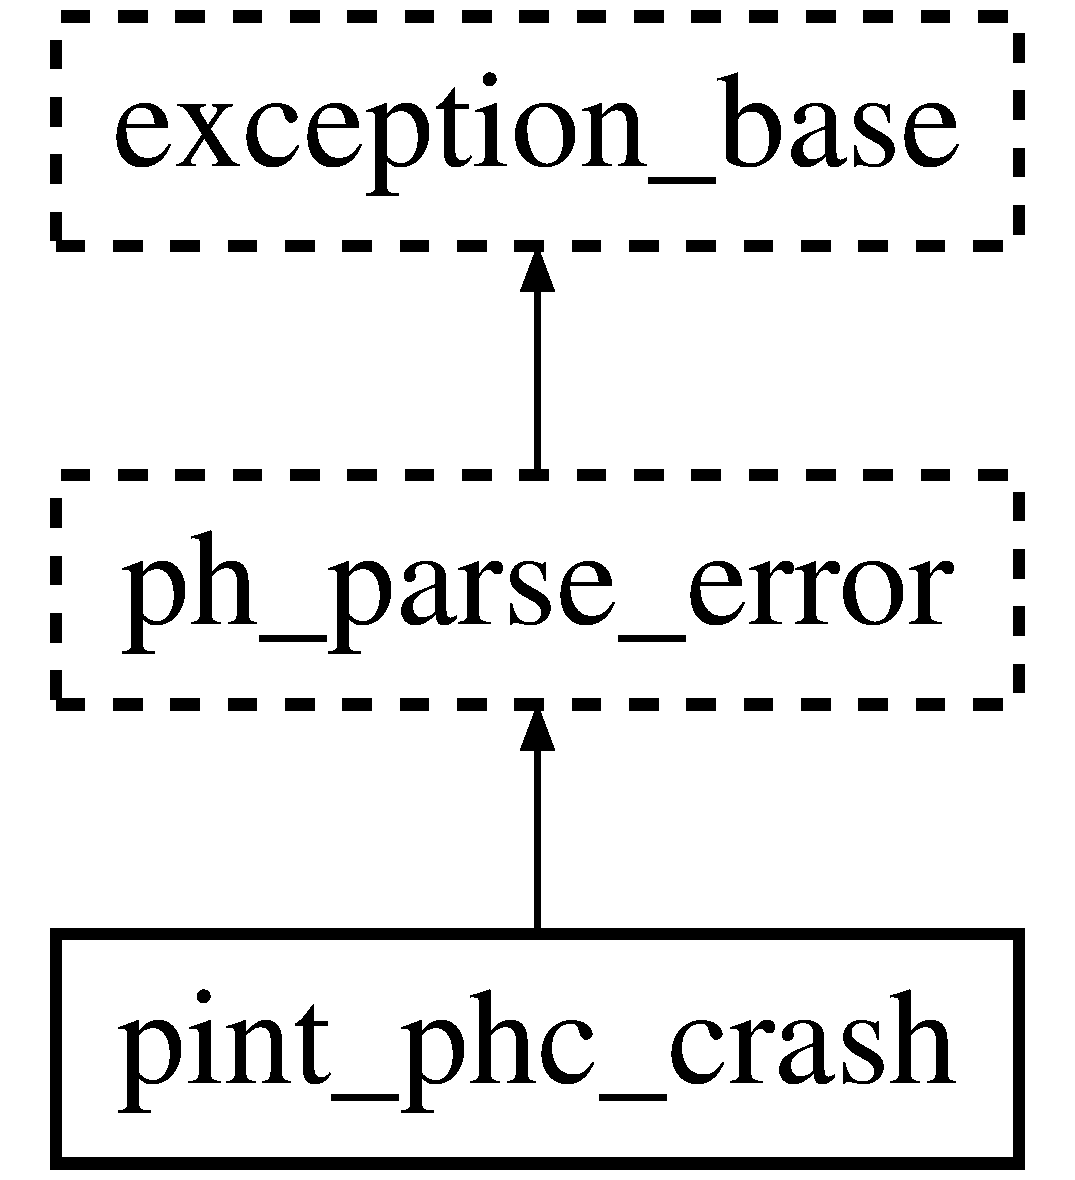
\includegraphics[height=3.000000cm]{structpint__phc__crash}
\end{center}
\end{figure}


\subsection{\-Detailed \-Description}
struct defining the exception called when \-Pint cannot be called extends \hyperlink{structph__parse__error}{ph\-\_\-parse\-\_\-error} 

\-The documentation for this class was generated from the following file\-:\begin{DoxyCompactItemize}
\item 
headers/\hyperlink{_exceptions_8h}{\-Exceptions.\-h}\end{DoxyCompactItemize}

\hypertarget{structpint__program__not__found}{\section{pint\-\_\-program\-\_\-not\-\_\-found \-Class \-Reference}
\label{structpint__program__not__found}\index{pint\-\_\-program\-\_\-not\-\_\-found@{pint\-\_\-program\-\_\-not\-\_\-found}}
}


struct defining the exception called when \-Pint is not found\$ extends \hyperlink{structexception__base}{exception\-\_\-base}  




{\ttfamily \#include $<$\-Exceptions.\-h$>$}

\-Inheritance diagram for pint\-\_\-program\-\_\-not\-\_\-found\-:\begin{figure}[H]
\begin{center}
\leavevmode
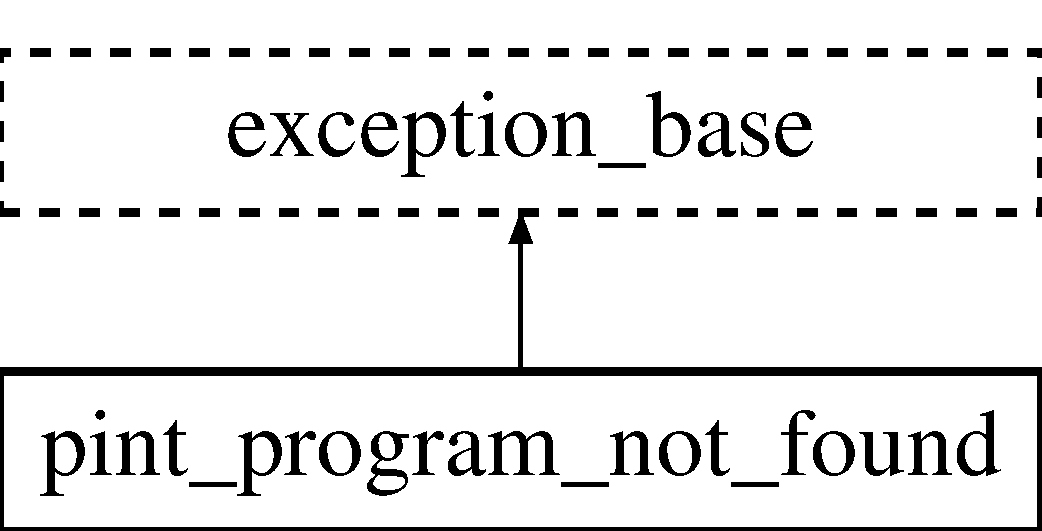
\includegraphics[height=2.000000cm]{structpint__program__not__found}
\end{center}
\end{figure}


\subsection{\-Detailed \-Description}
struct defining the exception called when \-Pint is not found\$ extends \hyperlink{structexception__base}{exception\-\_\-base} 

\-The documentation for this class was generated from the following file\-:\begin{DoxyCompactItemize}
\item 
headers/\hyperlink{_exceptions_8h}{\-Exceptions.\-h}\end{DoxyCompactItemize}

\hypertarget{class_process}{\section{\-Process \-Class \-Reference}
\label{class_process}\index{\-Process@{\-Process}}
}


represents a \hyperlink{class_process}{\-Process} of the process hitting  




{\ttfamily \#include $<$\-Process.\-h$>$}

\subsection*{\-Public \-Member \-Functions}
\begin{DoxyCompactItemize}
\item 
\hyperlink{class_process_a267617e8f2cfd994e0527635372be90c}{\-Process} (\-Sort\-Ptr s, const int \&n)
\begin{DoxyCompactList}\small\item\em constructor \end{DoxyCompactList}\item 
\hypertarget{class_process_acdfa357f41df6f1e09cdffbc5c5b2c3b}{int \hyperlink{class_process_acdfa357f41df6f1e09cdffbc5c5b2c3b}{get\-Number} (void)}\label{class_process_acdfa357f41df6f1e09cdffbc5c5b2c3b}

\begin{DoxyCompactList}\small\item\em gets the number \end{DoxyCompactList}\item 
\hypertarget{class_process_aaabe803350e1d6dcc23d8aa4ff2314db}{\-Sort\-Ptr \hyperlink{class_process_aaabe803350e1d6dcc23d8aa4ff2314db}{get\-Sort} (void)}\label{class_process_aaabe803350e1d6dcc23d8aa4ff2314db}

\begin{DoxyCompactList}\small\item\em gets the \hyperlink{class_sort}{\-Sort} \end{DoxyCompactList}\item 
string \hyperlink{class_process_af9a89e83db6a14451104b49eac7dd313}{get\-Dot\-Name} (void)
\begin{DoxyCompactList}\small\item\em builds name for \-D\-O\-T files \end{DoxyCompactList}\item 
string \hyperlink{class_process_ad9c1f2be57856c4e62d00f8494d2281f}{to\-Dot\-String} (void)
\begin{DoxyCompactList}\small\item\em gives a text representation of the process hitting (in .dot format, used in \-Graphviz) \end{DoxyCompactList}\item 
void \hyperlink{class_process_a14e32beee307cf814fbc569a96951bba}{set\-G\-Process} (\-G\-Process\-Ptr g\-P\-Ptr)
\begin{DoxyCompactList}\small\item\em sets the related \hyperlink{class_g_process}{\-G\-Process} \end{DoxyCompactList}\item 
\-G\-Process\-Ptr \hyperlink{class_process_af7c8dfd3af2a014c0371840ce82ed608}{get\-G\-Process} ()
\begin{DoxyCompactList}\small\item\em gets the related \hyperlink{class_g_process}{\-G\-Process} \end{DoxyCompactList}\end{DoxyCompactItemize}


\subsection{\-Detailed \-Description}
represents a \hyperlink{class_process}{\-Process} of the process hitting 

\subsection{\-Constructor \& \-Destructor \-Documentation}
\hypertarget{class_process_a267617e8f2cfd994e0527635372be90c}{\index{\-Process@{\-Process}!\-Process@{\-Process}}
\index{\-Process@{\-Process}!Process@{\-Process}}
\subsubsection[{\-Process}]{\setlength{\rightskip}{0pt plus 5cm}{\bf \-Process\-::\-Process} (
\begin{DoxyParamCaption}
\item[{\-Sort\-Ptr}]{s, }
\item[{const int \&}]{n}
\end{DoxyParamCaption}
)}}\label{class_process_a267617e8f2cfd994e0527635372be90c}


constructor 


\begin{DoxyParams}{\-Parameters}
{\em \-Sortptr} & pointer to the \hyperlink{class_sort}{\-Sort} the \hyperlink{class_process}{\-Process} is related to \\
\hline
{\em int} & number of the \hyperlink{class_process}{\-Process} in the \hyperlink{class_sort}{\-Sort} it is related to \\
\hline
\end{DoxyParams}


\subsection{\-Member \-Function \-Documentation}
\hypertarget{class_process_af9a89e83db6a14451104b49eac7dd313}{\index{\-Process@{\-Process}!get\-Dot\-Name@{get\-Dot\-Name}}
\index{get\-Dot\-Name@{get\-Dot\-Name}!Process@{\-Process}}
\subsubsection[{get\-Dot\-Name}]{\setlength{\rightskip}{0pt plus 5cm}string {\bf \-Process\-::get\-Dot\-Name} (
\begin{DoxyParamCaption}
\item[{void}]{}
\end{DoxyParamCaption}
)}}\label{class_process_af9a89e83db6a14451104b49eac7dd313}


builds name for \-D\-O\-T files 

\begin{DoxyReturn}{\-Returns}
string adapted name 
\end{DoxyReturn}
\hypertarget{class_process_af7c8dfd3af2a014c0371840ce82ed608}{\index{\-Process@{\-Process}!get\-G\-Process@{get\-G\-Process}}
\index{get\-G\-Process@{get\-G\-Process}!Process@{\-Process}}
\subsubsection[{get\-G\-Process}]{\setlength{\rightskip}{0pt plus 5cm}\-G\-Process\-Ptr {\bf \-Process\-::get\-G\-Process} (
\begin{DoxyParamCaption}
{}
\end{DoxyParamCaption}
)}}\label{class_process_af7c8dfd3af2a014c0371840ce82ed608}


gets the related \hyperlink{class_g_process}{\-G\-Process} 

\begin{DoxyReturn}{\-Returns}
\-G\-Process\-Ptr a pointer to the related \hyperlink{class_g_process}{\-G\-Process} object 
\end{DoxyReturn}
\hypertarget{class_process_a14e32beee307cf814fbc569a96951bba}{\index{\-Process@{\-Process}!set\-G\-Process@{set\-G\-Process}}
\index{set\-G\-Process@{set\-G\-Process}!Process@{\-Process}}
\subsubsection[{set\-G\-Process}]{\setlength{\rightskip}{0pt plus 5cm}void {\bf \-Process\-::set\-G\-Process} (
\begin{DoxyParamCaption}
\item[{\-G\-Process\-Ptr}]{g\-P\-Ptr}
\end{DoxyParamCaption}
)}}\label{class_process_a14e32beee307cf814fbc569a96951bba}


sets the related \hyperlink{class_g_process}{\-G\-Process} 


\begin{DoxyParams}{\-Parameters}
{\em a} & pointer to the related \hyperlink{class_g_process}{\-G\-Process} object \\
\hline
\end{DoxyParams}
\hypertarget{class_process_ad9c1f2be57856c4e62d00f8494d2281f}{\index{\-Process@{\-Process}!to\-Dot\-String@{to\-Dot\-String}}
\index{to\-Dot\-String@{to\-Dot\-String}!Process@{\-Process}}
\subsubsection[{to\-Dot\-String}]{\setlength{\rightskip}{0pt plus 5cm}string {\bf \-Process\-::to\-Dot\-String} (
\begin{DoxyParamCaption}
\item[{void}]{}
\end{DoxyParamCaption}
)}}\label{class_process_ad9c1f2be57856c4e62d00f8494d2281f}


gives a text representation of the process hitting (in .dot format, used in \-Graphviz) 

\begin{DoxyReturn}{\-Returns}
string the representation in \-D\-O\-T format 
\end{DoxyReturn}


\-The documentation for this class was generated from the following file\-:\begin{DoxyCompactItemize}
\item 
headers/\hyperlink{_process_8h}{\-Process.\-h}\end{DoxyCompactItemize}

\hypertarget{structprocess__not__found}{\section{process\-\_\-not\-\_\-found \-Class \-Reference}
\label{structprocess__not__found}\index{process\-\_\-not\-\_\-found@{process\-\_\-not\-\_\-found}}
}


struct defining the exception called when the process called is not found extends \hyperlink{structph__error}{ph\-\_\-error}  




{\ttfamily \#include $<$\-Exceptions.\-h$>$}

\-Inheritance diagram for process\-\_\-not\-\_\-found\-:\begin{figure}[H]
\begin{center}
\leavevmode
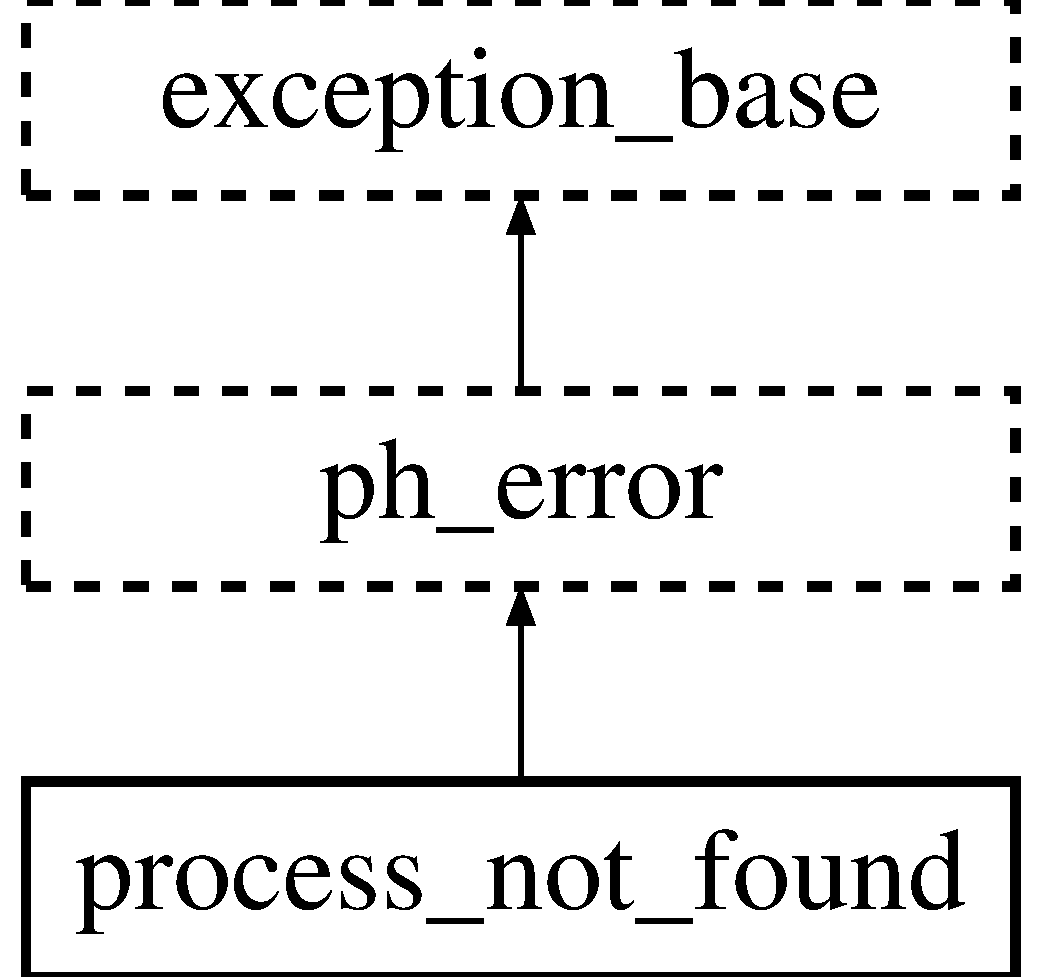
\includegraphics[height=3.000000cm]{structprocess__not__found}
\end{center}
\end{figure}


\subsection{\-Detailed \-Description}
struct defining the exception called when the process called is not found extends \hyperlink{structph__error}{ph\-\_\-error} 

\-The documentation for this class was generated from the following file\-:\begin{DoxyCompactItemize}
\item 
headers/\hyperlink{_exceptions_8h}{\-Exceptions.\-h}\end{DoxyCompactItemize}

\hypertarget{structprocess__required}{\section{process\-\_\-required \-Class \-Reference}
\label{structprocess__required}\index{process\-\_\-required@{process\-\_\-required}}
}


struct defining the exception called when the process is not specified extends \hyperlink{structph__error}{ph\-\_\-error}  




{\ttfamily \#include $<$\-Exceptions.\-h$>$}

\-Inheritance diagram for process\-\_\-required\-:\begin{figure}[H]
\begin{center}
\leavevmode
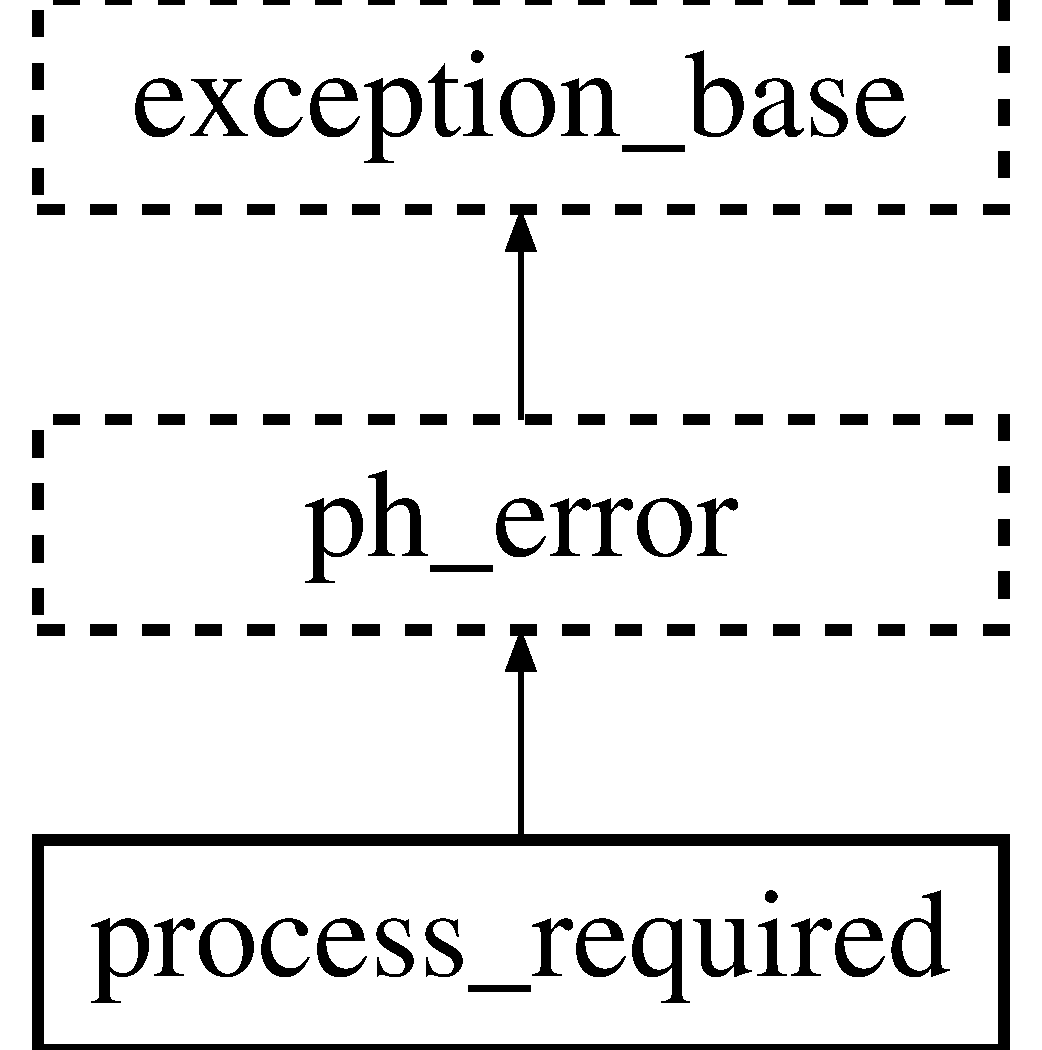
\includegraphics[height=3.000000cm]{structprocess__required}
\end{center}
\end{figure}


\subsection{\-Detailed \-Description}
struct defining the exception called when the process is not specified extends \hyperlink{structph__error}{ph\-\_\-error} 

\-The documentation for this class was generated from the following file\-:\begin{DoxyCompactItemize}
\item 
headers/\hyperlink{_exceptions_8h}{\-Exceptions.\-h}\end{DoxyCompactItemize}

\hypertarget{class_sort}{\section{\-Sort \-Class \-Reference}
\label{class_sort}\index{\-Sort@{\-Sort}}
}


represents a sort of the process hitting  




{\ttfamily \#include $<$\-Sort.\-h$>$}

\subsection*{\-Public \-Member \-Functions}
\begin{DoxyCompactItemize}
\item 
\-Process\-Ptr \hyperlink{class_sort_a5b30c6e6f75987a8a10bef36762aace6}{get\-Process} (const uint \&)
\begin{DoxyCompactList}\small\item\em gets a \hyperlink{class_process}{\-Process} by its index \end{DoxyCompactList}\item 
\hypertarget{class_sort_a1b76cf03a033bdee33ddd783e6e61f29}{vector$<$ \-Process\-Ptr $>$ \hyperlink{class_sort_a1b76cf03a033bdee33ddd783e6e61f29}{get\-Processes} (void)}\label{class_sort_a1b76cf03a033bdee33ddd783e6e61f29}

\begin{DoxyCompactList}\small\item\em gets processes vector \end{DoxyCompactList}\item 
\hypertarget{class_sort_ad77072a25565d843de3ea6a7b47ffbdd}{\-Process\-Ptr \hyperlink{class_sort_ad77072a25565d843de3ea6a7b47ffbdd}{get\-Active\-Process} (void)}\label{class_sort_ad77072a25565d843de3ea6a7b47ffbdd}

\begin{DoxyCompactList}\small\item\em gets the active process \end{DoxyCompactList}\item 
\hypertarget{class_sort_afb60d6f4e0b2d2984faf33fe16ad29b2}{void \hyperlink{class_sort_afb60d6f4e0b2d2984faf33fe16ad29b2}{set\-Active\-Process} (const int \&)}\label{class_sort_afb60d6f4e0b2d2984faf33fe16ad29b2}

\begin{DoxyCompactList}\small\item\em sets the active process \end{DoxyCompactList}\item 
int \hyperlink{class_sort_a1f91b39f9d5d05ffbf59a1480102e85c}{count\-Processes} (void)
\begin{DoxyCompactList}\small\item\em counts the number of processes \end{DoxyCompactList}\item 
\hypertarget{class_sort_aae171b005c3dada51b7a302230ff501a}{string \hyperlink{class_sort_aae171b005c3dada51b7a302230ff501a}{get\-Name} (void)}\label{class_sort_aae171b005c3dada51b7a302230ff501a}

\begin{DoxyCompactList}\small\item\em gets the name of the \hyperlink{class_sort}{\-Sort} \end{DoxyCompactList}\item 
string \hyperlink{class_sort_ae160613fb2d5c7fd9818a5c7d4be992a}{to\-String} (void)
\begin{DoxyCompactList}\small\item\em gives a text representation of the process hitting (as it would be in a .ph file) \end{DoxyCompactList}\item 
string \hyperlink{class_sort_a9bb67cd444d217dd477c896a31d869a0}{to\-Dot\-String} (void)
\begin{DoxyCompactList}\small\item\em gives a text representation of the process hitting (in .dot format, used in \-Graphviz) \end{DoxyCompactList}\end{DoxyCompactItemize}
\subsection*{\-Static \-Public \-Member \-Functions}
\begin{DoxyCompactItemize}
\item 
static \-Sort\-Ptr \hyperlink{class_sort_a9c3fa1c3b71839c425d99a7fa86a9cc2}{make} (const string \&, const int \&)
\begin{DoxyCompactList}\small\item\em creates a pointer to the \hyperlink{class_sort}{\-Sort} which name is given as parameter \end{DoxyCompactList}\end{DoxyCompactItemize}
\subsection*{\-Protected \-Member \-Functions}
\begin{DoxyCompactItemize}
\item 
\hypertarget{class_sort_ab9d3cb2bb873e058d0129e793c947d45}{\hyperlink{class_sort_ab9d3cb2bb873e058d0129e793c947d45}{\-Sort} (const string \&)}\label{class_sort_ab9d3cb2bb873e058d0129e793c947d45}

\begin{DoxyCompactList}\small\item\em constructor \end{DoxyCompactList}\item 
void \hyperlink{class_sort_a63bd04693623b2a269e76b9d5269e880}{add\-Process} (\-Process\-Ptr p)
\begin{DoxyCompactList}\small\item\em adds a \hyperlink{class_process}{\-Process} \end{DoxyCompactList}\end{DoxyCompactItemize}
\subsection*{\-Protected \-Attributes}
\begin{DoxyCompactItemize}
\item 
\hypertarget{class_sort_a047fd7c62ee90060e2e9374f6dc9ceca}{string \hyperlink{class_sort_a047fd7c62ee90060e2e9374f6dc9ceca}{name}}\label{class_sort_a047fd7c62ee90060e2e9374f6dc9ceca}

\begin{DoxyCompactList}\small\item\em name of the \hyperlink{class_sort}{\-Sort} \end{DoxyCompactList}\item 
\hypertarget{class_sort_abd772622b6c5b12de38d3a646258cc0a}{vector$<$ \-Process\-Ptr $>$ \hyperlink{class_sort_abd772622b6c5b12de38d3a646258cc0a}{processes}}\label{class_sort_abd772622b6c5b12de38d3a646258cc0a}

\begin{DoxyCompactList}\small\item\em \-Processes of the \hyperlink{class_sort}{\-Sort}. \end{DoxyCompactList}\item 
\hypertarget{class_sort_a941e734fb42ff8042ba0d4e82f22a9d8}{\-Process\-Ptr \hyperlink{class_sort_a941e734fb42ff8042ba0d4e82f22a9d8}{active\-Process}}\label{class_sort_a941e734fb42ff8042ba0d4e82f22a9d8}

\begin{DoxyCompactList}\small\item\em active \hyperlink{class_process}{\-Process} in the \hyperlink{class_sort}{\-Sort} \end{DoxyCompactList}\end{DoxyCompactItemize}


\subsection{\-Detailed \-Description}
represents a sort of the process hitting 

\subsection{\-Member \-Function \-Documentation}
\hypertarget{class_sort_a63bd04693623b2a269e76b9d5269e880}{\index{\-Sort@{\-Sort}!add\-Process@{add\-Process}}
\index{add\-Process@{add\-Process}!Sort@{\-Sort}}
\subsubsection[{add\-Process}]{\setlength{\rightskip}{0pt plus 5cm}void {\bf \-Sort\-::add\-Process} (
\begin{DoxyParamCaption}
\item[{\-Process\-Ptr}]{p}
\end{DoxyParamCaption}
)\hspace{0.3cm}{\ttfamily  \mbox{[}protected\mbox{]}}}}\label{class_sort_a63bd04693623b2a269e76b9d5269e880}


adds a \hyperlink{class_process}{\-Process} 


\begin{DoxyParams}{\-Parameters}
{\em \-Process\-Ptr} & pointer to the \hyperlink{class_process}{\-Process} to add \\
\hline
\end{DoxyParams}
\hypertarget{class_sort_a1f91b39f9d5d05ffbf59a1480102e85c}{\index{\-Sort@{\-Sort}!count\-Processes@{count\-Processes}}
\index{count\-Processes@{count\-Processes}!Sort@{\-Sort}}
\subsubsection[{count\-Processes}]{\setlength{\rightskip}{0pt plus 5cm}int {\bf \-Sort\-::count\-Processes} (
\begin{DoxyParamCaption}
\item[{void}]{}
\end{DoxyParamCaption}
)}}\label{class_sort_a1f91b39f9d5d05ffbf59a1480102e85c}


counts the number of processes 

\begin{DoxyReturn}{\-Returns}
int the number of processes 
\end{DoxyReturn}
\hypertarget{class_sort_a5b30c6e6f75987a8a10bef36762aace6}{\index{\-Sort@{\-Sort}!get\-Process@{get\-Process}}
\index{get\-Process@{get\-Process}!Sort@{\-Sort}}
\subsubsection[{get\-Process}]{\setlength{\rightskip}{0pt plus 5cm}\-Process\-Ptr {\bf \-Sort\-::get\-Process} (
\begin{DoxyParamCaption}
\item[{const uint \&}]{}
\end{DoxyParamCaption}
)}}\label{class_sort_a5b30c6e6f75987a8a10bef36762aace6}


gets a \hyperlink{class_process}{\-Process} by its index 


\begin{DoxyParams}{\-Parameters}
{\em uint} & the index of the \hyperlink{class_process}{\-Process} in processes vector \\
\hline
\end{DoxyParams}
\hypertarget{class_sort_a9c3fa1c3b71839c425d99a7fa86a9cc2}{\index{\-Sort@{\-Sort}!make@{make}}
\index{make@{make}!Sort@{\-Sort}}
\subsubsection[{make}]{\setlength{\rightskip}{0pt plus 5cm}static \-Sort\-Ptr {\bf \-Sort\-::make} (
\begin{DoxyParamCaption}
\item[{const string \&}]{, }
\item[{const int \&}]{}
\end{DoxyParamCaption}
)\hspace{0.3cm}{\ttfamily  \mbox{[}static\mbox{]}}}}\label{class_sort_a9c3fa1c3b71839c425d99a7fa86a9cc2}


creates a pointer to the \hyperlink{class_sort}{\-Sort} which name is given as parameter 


\begin{DoxyParams}{\-Parameters}
{\em string} & name of the \hyperlink{class_sort}{\-Sort} to created \\
\hline
{\em int} & number of processes in the \hyperlink{class_sort}{\-Sort} \\
\hline
\end{DoxyParams}
\begin{DoxyReturn}{\-Returns}
\-Sort\-Ptr the pointer to the created \hyperlink{class_sort}{\-Sort} 
\end{DoxyReturn}
\hypertarget{class_sort_a9bb67cd444d217dd477c896a31d869a0}{\index{\-Sort@{\-Sort}!to\-Dot\-String@{to\-Dot\-String}}
\index{to\-Dot\-String@{to\-Dot\-String}!Sort@{\-Sort}}
\subsubsection[{to\-Dot\-String}]{\setlength{\rightskip}{0pt plus 5cm}string {\bf \-Sort\-::to\-Dot\-String} (
\begin{DoxyParamCaption}
\item[{void}]{}
\end{DoxyParamCaption}
)}}\label{class_sort_a9bb67cd444d217dd477c896a31d869a0}


gives a text representation of the process hitting (in .dot format, used in \-Graphviz) 

\begin{DoxyReturn}{\-Returns}
string the text representation of the process hitting in \-D\-O\-T format 
\end{DoxyReturn}
\hypertarget{class_sort_ae160613fb2d5c7fd9818a5c7d4be992a}{\index{\-Sort@{\-Sort}!to\-String@{to\-String}}
\index{to\-String@{to\-String}!Sort@{\-Sort}}
\subsubsection[{to\-String}]{\setlength{\rightskip}{0pt plus 5cm}string {\bf \-Sort\-::to\-String} (
\begin{DoxyParamCaption}
\item[{void}]{}
\end{DoxyParamCaption}
)}}\label{class_sort_ae160613fb2d5c7fd9818a5c7d4be992a}


gives a text representation of the process hitting (as it would be in a .ph file) 

\begin{DoxyReturn}{\-Returns}
string the text representation of the process hitting in \hyperlink{class_p_h}{\-P\-H} format 
\end{DoxyReturn}


\-The documentation for this class was generated from the following file\-:\begin{DoxyCompactItemize}
\item 
headers/\hyperlink{_sort_8h}{\-Sort.\-h}\end{DoxyCompactItemize}

\hypertarget{structsort__not__found}{\section{sort\-\_\-not\-\_\-found \-Class \-Reference}
\label{structsort__not__found}\index{sort\-\_\-not\-\_\-found@{sort\-\_\-not\-\_\-found}}
}


struct defining the exception called when the sort called are not found extends \hyperlink{structph__error}{ph\-\_\-error}  




{\ttfamily \#include $<$\-Exceptions.\-h$>$}

\-Inheritance diagram for sort\-\_\-not\-\_\-found\-:\begin{figure}[H]
\begin{center}
\leavevmode
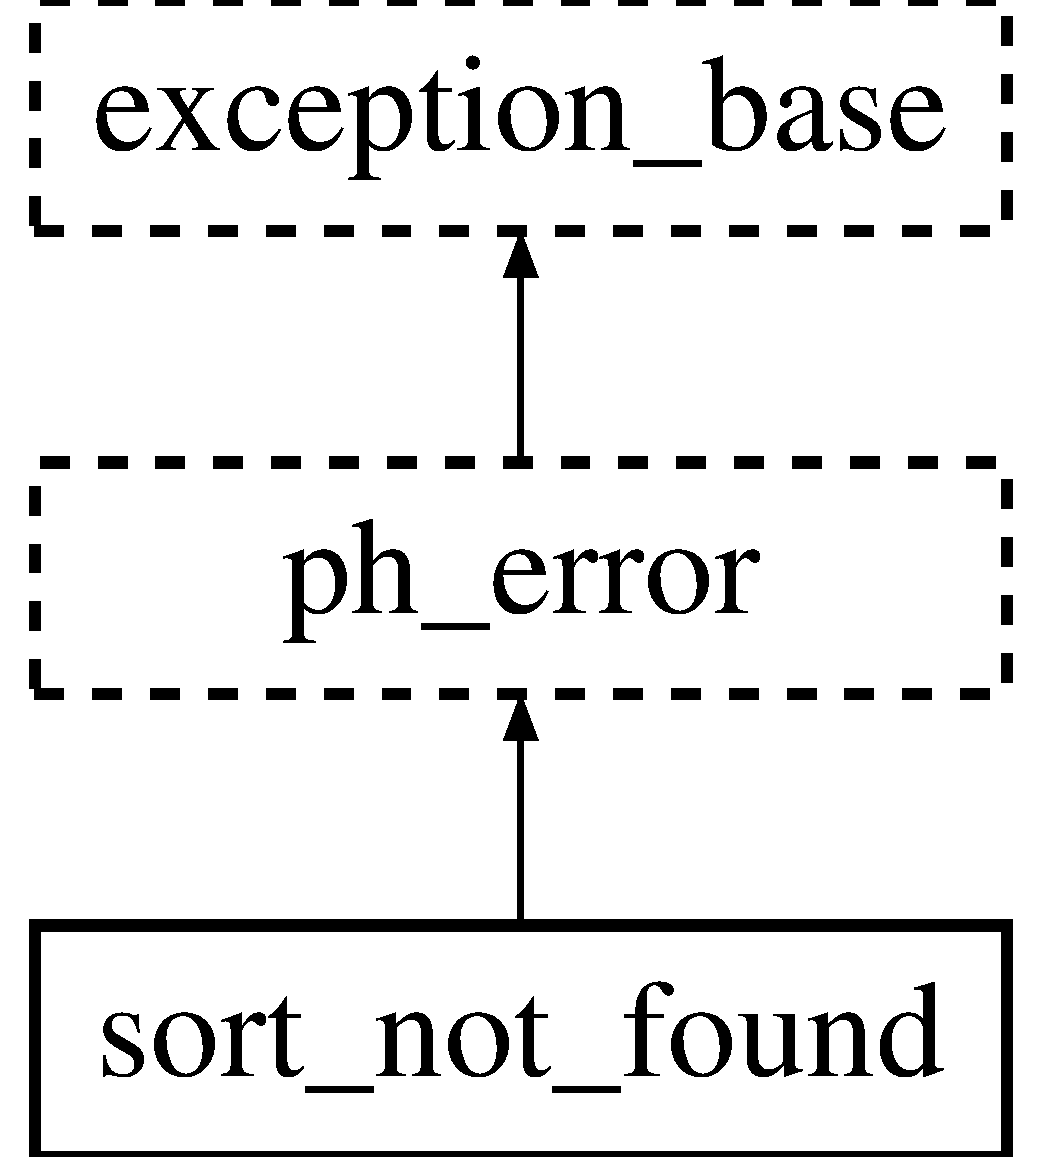
\includegraphics[height=3.000000cm]{structsort__not__found}
\end{center}
\end{figure}


\subsection{\-Detailed \-Description}
struct defining the exception called when the sort called are not found extends \hyperlink{structph__error}{ph\-\_\-error} 

\-The documentation for this class was generated from the following file\-:\begin{DoxyCompactItemize}
\item 
headers/\hyperlink{_exceptions_8h}{\-Exceptions.\-h}\end{DoxyCompactItemize}

\hypertarget{structsubgraph__not__found}{\section{subgraph\-\_\-not\-\_\-found \-Class \-Reference}
\label{structsubgraph__not__found}\index{subgraph\-\_\-not\-\_\-found@{subgraph\-\_\-not\-\_\-found}}
}


struct defining the exception called when the subgraph is not found extends \hyperlink{structgv__error}{gv\-\_\-error}  




{\ttfamily \#include $<$\-Exceptions.\-h$>$}

\-Inheritance diagram for subgraph\-\_\-not\-\_\-found\-:\begin{figure}[H]
\begin{center}
\leavevmode
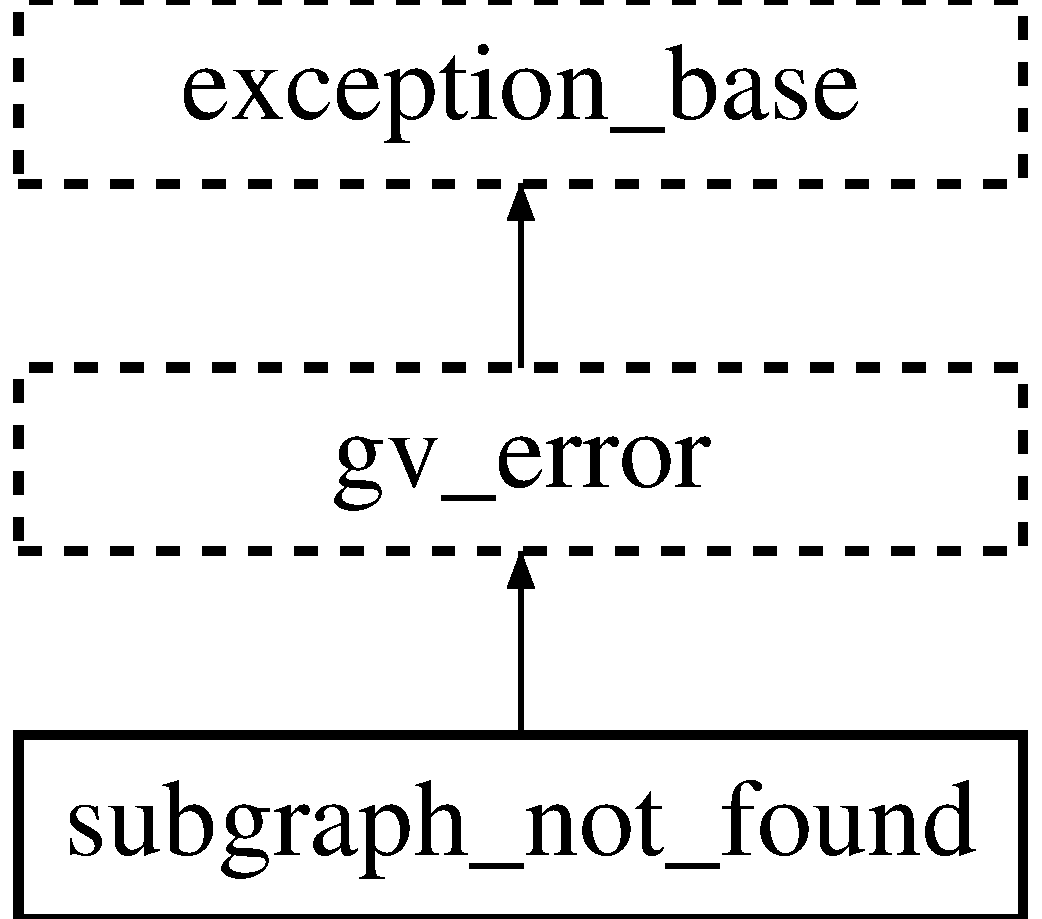
\includegraphics[height=3.000000cm]{structsubgraph__not__found}
\end{center}
\end{figure}


\subsection{\-Detailed \-Description}
struct defining the exception called when the subgraph is not found extends \hyperlink{structgv__error}{gv\-\_\-error} 

\-The documentation for this class was generated from the following file\-:\begin{DoxyCompactItemize}
\item 
headers/\hyperlink{_exceptions_8h}{\-Exceptions.\-h}\end{DoxyCompactItemize}

\hypertarget{class_text_area}{\section{\-Text\-Area \-Class \-Reference}
\label{class_text_area}\index{\-Text\-Area@{\-Text\-Area}}
}


\-Text \-Widget extends \-Q\-Text\-Edit.  




{\ttfamily \#include $<$\-Text\-Area.\-h$>$}

\subsection*{\-Public \-Member \-Functions}
\begin{DoxyCompactItemize}
\item 
\hyperlink{class_text_area_a1e6e009ccaa04030d35f9187a37fe4da}{\-Text\-Area} (\-Q\-Widget $\ast$parent)
\begin{DoxyCompactList}\small\item\em constructor \end{DoxyCompactList}\item 
\hypertarget{class_text_area_acdfa220612113b805f8653dce6b7624e}{void \hyperlink{class_text_area_acdfa220612113b805f8653dce6b7624e}{change\-Background\-Color} (\-Q\-Color)}\label{class_text_area_acdfa220612113b805f8653dce6b7624e}

\begin{DoxyCompactList}\small\item\em changes the text widget background color, called from a signal in the main window \end{DoxyCompactList}\end{DoxyCompactItemize}


\subsection{\-Detailed \-Description}
\-Text \-Widget extends \-Q\-Text\-Edit. 

\subsection{\-Constructor \& \-Destructor \-Documentation}
\hypertarget{class_text_area_a1e6e009ccaa04030d35f9187a37fe4da}{\index{\-Text\-Area@{\-Text\-Area}!\-Text\-Area@{\-Text\-Area}}
\index{\-Text\-Area@{\-Text\-Area}!TextArea@{\-Text\-Area}}
\subsubsection[{\-Text\-Area}]{\setlength{\rightskip}{0pt plus 5cm}{\bf \-Text\-Area\-::\-Text\-Area} (
\begin{DoxyParamCaption}
\item[{\-Q\-Widget $\ast$}]{parent}
\end{DoxyParamCaption}
)}}\label{class_text_area_a1e6e009ccaa04030d35f9187a37fe4da}


constructor 

\-Q\-Widget parent, the widget containing the \hyperlink{class_text_area}{\-Text\-Area}, which is the \hyperlink{class_area}{\-Area} 

\-The documentation for this class was generated from the following file\-:\begin{DoxyCompactItemize}
\item 
headers/\-Text\-Area.\-h\end{DoxyCompactItemize}

\hypertarget{class_tree_area}{\section{\-Tree\-Area \-Class \-Reference}
\label{class_tree_area}\index{\-Tree\-Area@{\-Tree\-Area}}
}


\-Tree \-Wigets extends \-Q\-Widget.  




{\ttfamily \#include $<$\-Tree\-Area.\-h$>$}

\subsection*{\-Public \-Slots}
\begin{DoxyCompactItemize}
\item 
\hypertarget{class_tree_area_a8fd7c22b1c8c4e8cb9503731d66c5d47}{void \hyperlink{class_tree_area_a8fd7c22b1c8c4e8cb9503731d66c5d47}{build} ()}\label{class_tree_area_a8fd7c22b1c8c4e8cb9503731d66c5d47}

\begin{DoxyCompactList}\small\item\em build the base tree. \-Called on opening \end{DoxyCompactList}\item 
\hypertarget{class_tree_area_aee1ca64b79821f9cbcc023861e169e33}{void \hyperlink{class_tree_area_aee1ca64b79821f9cbcc023861e169e33}{search\-Sort} ()}\label{class_tree_area_aee1ca64b79821f9cbcc023861e169e33}

\begin{DoxyCompactList}\small\item\em search a sort. \-Slot linked with the search button signal \end{DoxyCompactList}\item 
\hypertarget{class_tree_area_a4dc4bffd318bcf5a4023ec92a4932214}{void \hyperlink{class_tree_area_a4dc4bffd318bcf5a4023ec92a4932214}{cancel\-Search} ()}\label{class_tree_area_a4dc4bffd318bcf5a4023ec92a4932214}

\begin{DoxyCompactList}\small\item\em cancel the search of the sort. \-Shows all the items in the tree \end{DoxyCompactList}\item 
\hypertarget{class_tree_area_a1825d29fa6bd5fbf4e8c0a4f657284bd}{void \hyperlink{class_tree_area_a1825d29fa6bd5fbf4e8c0a4f657284bd}{add\-Group} ()}\label{class_tree_area_a1825d29fa6bd5fbf4e8c0a4f657284bd}

\begin{DoxyCompactList}\small\item\em add a group to the groups\-Tree \end{DoxyCompactList}\item 
\hypertarget{class_tree_area_af231946c277606cf3613f82ffd859a01}{void \hyperlink{class_tree_area_af231946c277606cf3613f82ffd859a01}{remove} ()}\label{class_tree_area_af231946c277606cf3613f82ffd859a01}

\begin{DoxyCompactList}\small\item\em remove the selected group from the groups\-Tree \end{DoxyCompactList}\item 
\hypertarget{class_tree_area_a47f535fca68dd94484227f4669cc773d}{void \hyperlink{class_tree_area_a47f535fca68dd94484227f4669cc773d}{add\-To\-Group} ()}\label{class_tree_area_a47f535fca68dd94484227f4669cc773d}

\begin{DoxyCompactList}\small\item\em add a sort to a selected group \end{DoxyCompactList}\item 
\hypertarget{class_tree_area_a8a8afdc75c8e16720f9dde739d1f53e0}{void \hyperlink{class_tree_area_a8a8afdc75c8e16720f9dde739d1f53e0}{sorts\-Item\-Clicked} (const \-Q\-Point \&pos)}\label{class_tree_area_a8a8afdc75c8e16720f9dde739d1f53e0}

\begin{DoxyCompactList}\small\item\em menu to show when the sort is clicked \end{DoxyCompactList}\item 
void \hyperlink{class_tree_area_ad8651281efec4086ec668b43f1d528d9}{hide\-Sort} (int clicked\-Tree)
\begin{DoxyCompactList}\small\item\em hide a sort \end{DoxyCompactList}\item 
void \hyperlink{class_tree_area_a89ea1654d33d7d83a7bbb8b3a79b60ad}{show\-Sort} (int clicked\-Tree)
\begin{DoxyCompactList}\small\item\em show a sort \end{DoxyCompactList}\item 
void \hyperlink{class_tree_area_a5277c42469c5dab4cc117441ed2d872a}{change\-Sort\-Color} (int clicked\-Tree)
\begin{DoxyCompactList}\small\item\em change sort color \end{DoxyCompactList}\item 
\hypertarget{class_tree_area_a5eb847a42ee5dbcdbfc8d419b322197e}{void \hyperlink{class_tree_area_a5eb847a42ee5dbcdbfc8d419b322197e}{change\-Sort\-Rect\-Color} (\-Q\-Tree\-Widget\-Item $\ast$, \-Q\-Color $\ast$)}\label{class_tree_area_a5eb847a42ee5dbcdbfc8d419b322197e}

\begin{DoxyCompactList}\small\item\em change sort's rect color \end{DoxyCompactList}\item 
\hypertarget{class_tree_area_a1a3c713057c8aee75749706af8ad3cf6}{void \hyperlink{class_tree_area_a1a3c713057c8aee75749706af8ad3cf6}{groups\-Item\-Clicked} (const \-Q\-Point \&pos)}\label{class_tree_area_a1a3c713057c8aee75749706af8ad3cf6}

\begin{DoxyCompactList}\small\item\em menu to show when the sort is clicked \end{DoxyCompactList}\item 
\hypertarget{class_tree_area_a7ec5a5d26a01615f6cc9acac55fd745e}{void \hyperlink{class_tree_area_a7ec5a5d26a01615f6cc9acac55fd745e}{hide\-Group} ()}\label{class_tree_area_a7ec5a5d26a01615f6cc9acac55fd745e}

\begin{DoxyCompactList}\small\item\em hide a sort \end{DoxyCompactList}\item 
\hypertarget{class_tree_area_a676a80fa10cb0d43a4bef32180679c2b}{void \hyperlink{class_tree_area_a676a80fa10cb0d43a4bef32180679c2b}{show\-Group} ()}\label{class_tree_area_a676a80fa10cb0d43a4bef32180679c2b}

\begin{DoxyCompactList}\small\item\em show a sort \end{DoxyCompactList}\item 
\hypertarget{class_tree_area_ac59ce87a367e3b0657718a57b718760d}{void \hyperlink{class_tree_area_ac59ce87a367e3b0657718a57b718760d}{change\-Group\-Color} ()}\label{class_tree_area_ac59ce87a367e3b0657718a57b718760d}

\begin{DoxyCompactList}\small\item\em change sort color \end{DoxyCompactList}\item 
\hypertarget{class_tree_area_adf29861998cba6d9ae174a50c37a7fac}{void \hyperlink{class_tree_area_adf29861998cba6d9ae174a50c37a7fac}{hide\-Sort\-Clicked\-From\-Sort} ()}\label{class_tree_area_adf29861998cba6d9ae174a50c37a7fac}

\begin{DoxyCompactList}\small\item\em slot signifying that the item is clicked from the sorts\-Tree and calls hide\-Sort(1) \end{DoxyCompactList}\item 
\hypertarget{class_tree_area_a78a3ddc89efe14b41c825adb727dfdc6}{void \hyperlink{class_tree_area_a78a3ddc89efe14b41c825adb727dfdc6}{show\-Sort\-Clicked\-From\-Sort} ()}\label{class_tree_area_a78a3ddc89efe14b41c825adb727dfdc6}

\begin{DoxyCompactList}\small\item\em slot signifying that the item is clicked from the sorts\-Tree and calls show\-Sort(1) \end{DoxyCompactList}\item 
\hypertarget{class_tree_area_a961bd8aaf9272cc4c669b624d2e1fd96}{void \hyperlink{class_tree_area_a961bd8aaf9272cc4c669b624d2e1fd96}{change\-Sort\-Color\-Clicked\-From\-Sort} ()}\label{class_tree_area_a961bd8aaf9272cc4c669b624d2e1fd96}

\begin{DoxyCompactList}\small\item\em slot signifying that the item is clicked from the sorts\-Tree and calls change\-Sort\-Color(1) \end{DoxyCompactList}\item 
\hypertarget{class_tree_area_ab5c0a22f1ccceb2244cb31f320971938}{void \hyperlink{class_tree_area_ab5c0a22f1ccceb2244cb31f320971938}{hide\-Sort\-Clicked\-From\-Group} ()}\label{class_tree_area_ab5c0a22f1ccceb2244cb31f320971938}

\begin{DoxyCompactList}\small\item\em slot signifying that the item is clicked from the groups\-Tree and calls hide\-Sort(2) \end{DoxyCompactList}\item 
\hypertarget{class_tree_area_ada5feadb41bb5cb913e253433e935107}{void \hyperlink{class_tree_area_ada5feadb41bb5cb913e253433e935107}{show\-Sort\-Clicked\-From\-Group} ()}\label{class_tree_area_ada5feadb41bb5cb913e253433e935107}

\begin{DoxyCompactList}\small\item\em slot signifying that the item is clicked from the groups\-Tree and calls show\-Sort(2) \end{DoxyCompactList}\item 
\hypertarget{class_tree_area_a393f334d7da481b4233ceb9912791c99}{void \hyperlink{class_tree_area_a393f334d7da481b4233ceb9912791c99}{change\-Sort\-Color\-Clicked\-From\-Group} ()}\label{class_tree_area_a393f334d7da481b4233ceb9912791c99}

\begin{DoxyCompactList}\small\item\em slot signifying that the item is clicked from the groups\-Tree and calls change\-Sort\-Color(2) \end{DoxyCompactList}\end{DoxyCompactItemize}
\subsection*{\-Public \-Member \-Functions}
\begin{DoxyCompactItemize}
\item 
\hyperlink{class_tree_area_a83e789309721c85ff2f431c789c641ec}{\-Tree\-Area} (\-Q\-Widget $\ast$parent)
\begin{DoxyCompactList}\small\item\em constructor \end{DoxyCompactList}\end{DoxyCompactItemize}
\subsection*{\-Public \-Attributes}
\begin{DoxyCompactItemize}
\item 
\hypertarget{class_tree_area_a290d659da16085f21c04f81fcd16891c}{\-P\-H\-Ptr \hyperlink{class_tree_area_a290d659da16085f21c04f81fcd16891c}{my\-P\-H\-Ptr}}\label{class_tree_area_a290d659da16085f21c04f81fcd16891c}

\begin{DoxyCompactList}\small\item\em pointer to the \hyperlink{class_p_h}{\-P\-H} \end{DoxyCompactList}\item 
\hypertarget{class_tree_area_a1bd090dc9ab10415e8f897b6300bc555}{\hyperlink{class_my_area}{\-My\-Area} $\ast$ \hyperlink{class_tree_area_a1bd090dc9ab10415e8f897b6300bc555}{my\-Area}}\label{class_tree_area_a1bd090dc9ab10415e8f897b6300bc555}

\begin{DoxyCompactList}\small\item\em pointer to the my\-Area \end{DoxyCompactList}\item 
\hypertarget{class_tree_area_ad323879d9e2e64b18dae18fe757b1b0e}{\-Q\-Tree\-Widget $\ast$ \hyperlink{class_tree_area_ad323879d9e2e64b18dae18fe757b1b0e}{sorts\-Tree}}\label{class_tree_area_ad323879d9e2e64b18dae18fe757b1b0e}

\begin{DoxyCompactList}\small\item\em pointer to the sorts \-Q\-Tree\-Widget \end{DoxyCompactList}\item 
\hypertarget{class_tree_area_ab3cf8ca35655b0bace24a7c46170852f}{\-Q\-Tree\-Widget $\ast$ \hyperlink{class_tree_area_ab3cf8ca35655b0bace24a7c46170852f}{groups\-Tree}}\label{class_tree_area_ab3cf8ca35655b0bace24a7c46170852f}

\begin{DoxyCompactList}\small\item\em pointer to the groups \-Q\-Tree\-Widget \end{DoxyCompactList}\item 
\hypertarget{class_tree_area_a682ba9e29364cbfca7ad726a6a630907}{\-Q\-Push\-Button $\ast$ \hyperlink{class_tree_area_a682ba9e29364cbfca7ad726a6a630907}{search\-Button}}\label{class_tree_area_a682ba9e29364cbfca7ad726a6a630907}

\begin{DoxyCompactList}\small\item\em pointer to the search button \end{DoxyCompactList}\item 
\hypertarget{class_tree_area_a740ea34ee424f43171bcdd69125e515e}{\-Q\-Push\-Button $\ast$ \hyperlink{class_tree_area_a740ea34ee424f43171bcdd69125e515e}{cancel\-Search\-Button}}\label{class_tree_area_a740ea34ee424f43171bcdd69125e515e}

\begin{DoxyCompactList}\small\item\em pointer to the cancel\-Search button \end{DoxyCompactList}\item 
\hypertarget{class_tree_area_a609dd67c5b1d7bb8d0661054338f9561}{\-Q\-Line\-Edit $\ast$ \hyperlink{class_tree_area_a609dd67c5b1d7bb8d0661054338f9561}{search\-Box}}\label{class_tree_area_a609dd67c5b1d7bb8d0661054338f9561}

\begin{DoxyCompactList}\small\item\em pointer to the search line edit \end{DoxyCompactList}\item 
\hypertarget{class_tree_area_ab77bb00c229d79b09736ff7948f1fc32}{\-Q\-Push\-Button $\ast$ \hyperlink{class_tree_area_ab77bb00c229d79b09736ff7948f1fc32}{add\-To\-Group\-Button}}\label{class_tree_area_ab77bb00c229d79b09736ff7948f1fc32}

\begin{DoxyCompactList}\small\item\em pointer to the add\-To\-Group button \end{DoxyCompactList}\item 
\hypertarget{class_tree_area_ab1bb8dfaad1425a3b1fcd48f75f140f2}{\-Q\-Push\-Button $\ast$ \hyperlink{class_tree_area_ab1bb8dfaad1425a3b1fcd48f75f140f2}{remove\-Group\-Button}}\label{class_tree_area_ab1bb8dfaad1425a3b1fcd48f75f140f2}

\begin{DoxyCompactList}\small\item\em pointer to the remove\-Group button \end{DoxyCompactList}\item 
\hypertarget{class_tree_area_a6e20bfd0bba99c036d7909d246a3fffa}{\-Q\-Push\-Button $\ast$ \hyperlink{class_tree_area_a6e20bfd0bba99c036d7909d246a3fffa}{add\-Group\-Button}}\label{class_tree_area_a6e20bfd0bba99c036d7909d246a3fffa}

\begin{DoxyCompactList}\small\item\em pointer to the add\-Group button \end{DoxyCompactList}\item 
\hypertarget{class_tree_area_a5a049742466ca1b4d0157f866f478e18}{\-Q\-List$<$ \-Q\-Tree\-Widget\-Item $\ast$ $>$ \hyperlink{class_tree_area_a5a049742466ca1b4d0157f866f478e18}{sorts}}\label{class_tree_area_a5a049742466ca1b4d0157f866f478e18}

\begin{DoxyCompactList}\small\item\em list containing all the sorts. \-Built when the file is opened \end{DoxyCompactList}\item 
\hypertarget{class_tree_area_a49fbc4c7f782976aa082896909c6a351}{\-Q\-List$<$ \-Q\-Tree\-Widget\-Item $\ast$ $>$ \hyperlink{class_tree_area_a49fbc4c7f782976aa082896909c6a351}{groups}}\label{class_tree_area_a49fbc4c7f782976aa082896909c6a351}

\begin{DoxyCompactList}\small\item\em list containing all the groups. \end{DoxyCompactList}\item 
\hypertarget{class_tree_area_a965d3a0fa45f6e31a50db967598f0f90}{\-Q\-Map$<$ \-Q\-Tree\-Widget\-Item $\ast$, \-Q\-Color $>$ $\ast$ \hyperlink{class_tree_area_a965d3a0fa45f6e31a50db967598f0f90}{groups\-Palette}}\label{class_tree_area_a965d3a0fa45f6e31a50db967598f0f90}

\begin{DoxyCompactList}\small\item\em map containing the colors of the groups \end{DoxyCompactList}\item 
\hypertarget{class_tree_area_a7e464d23da2120350b488e1828c13071}{\-Q\-List$<$ \-Q\-Color $>$ $\ast$ \hyperlink{class_tree_area_a7e464d23da2120350b488e1828c13071}{palette}}\label{class_tree_area_a7e464d23da2120350b488e1828c13071}

\begin{DoxyCompactList}\small\item\em list containing the standard colors for the groups \end{DoxyCompactList}\end{DoxyCompactItemize}
\subsection*{\-Static \-Public \-Attributes}
\begin{DoxyCompactItemize}
\item 
\hypertarget{class_tree_area_a580e62f552dbda007c636bc69cc5e0a7}{static const int \hyperlink{class_tree_area_a580e62f552dbda007c636bc69cc5e0a7}{click\-In\-Sorts\-Tree}}\label{class_tree_area_a580e62f552dbda007c636bc69cc5e0a7}

\begin{DoxyCompactList}\small\item\em flag that indicates that user clicked an item in sorts\-Tree \end{DoxyCompactList}\item 
\hypertarget{class_tree_area_a6c8a68ece69178b1c902cf8ee8652756}{static const int \hyperlink{class_tree_area_a6c8a68ece69178b1c902cf8ee8652756}{click\-In\-Groups\-Tree}}\label{class_tree_area_a6c8a68ece69178b1c902cf8ee8652756}

\begin{DoxyCompactList}\small\item\em flag that indicates that user clicked an item in groups\-Tree \end{DoxyCompactList}\end{DoxyCompactItemize}


\subsection{\-Detailed \-Description}
\-Tree \-Wigets extends \-Q\-Widget. 

\subsection{\-Constructor \& \-Destructor \-Documentation}
\hypertarget{class_tree_area_a83e789309721c85ff2f431c789c641ec}{\index{\-Tree\-Area@{\-Tree\-Area}!\-Tree\-Area@{\-Tree\-Area}}
\index{\-Tree\-Area@{\-Tree\-Area}!TreeArea@{\-Tree\-Area}}
\subsubsection[{\-Tree\-Area}]{\setlength{\rightskip}{0pt plus 5cm}{\bf \-Tree\-Area\-::\-Tree\-Area} (
\begin{DoxyParamCaption}
\item[{\-Q\-Widget $\ast$}]{parent}
\end{DoxyParamCaption}
)}}\label{class_tree_area_a83e789309721c85ff2f431c789c641ec}


constructor 

\-Q\-Widget parent, the widget containing the \hyperlink{class_text_area}{\-Text\-Area}, which is the \hyperlink{class_area}{\-Area} 

\subsection{\-Member \-Function \-Documentation}
\hypertarget{class_tree_area_a5277c42469c5dab4cc117441ed2d872a}{\index{\-Tree\-Area@{\-Tree\-Area}!change\-Sort\-Color@{change\-Sort\-Color}}
\index{change\-Sort\-Color@{change\-Sort\-Color}!TreeArea@{\-Tree\-Area}}
\subsubsection[{change\-Sort\-Color}]{\setlength{\rightskip}{0pt plus 5cm}void {\bf \-Tree\-Area\-::change\-Sort\-Color} (
\begin{DoxyParamCaption}
\item[{int}]{clicked\-Tree}
\end{DoxyParamCaption}
)\hspace{0.3cm}{\ttfamily  \mbox{[}slot\mbox{]}}}}\label{class_tree_area_a5277c42469c5dab4cc117441ed2d872a}


change sort color 


\begin{DoxyParams}{\-Parameters}
{\em int} & a flag that takes the value \hyperlink{class_tree_area_a580e62f552dbda007c636bc69cc5e0a7}{\-Tree\-Area\-::click\-In\-Sorts\-Tree} or \hyperlink{class_tree_area_a6c8a68ece69178b1c902cf8ee8652756}{\-Tree\-Area\-::click\-In\-Groups\-Tree} \\
\hline
\end{DoxyParams}
\hypertarget{class_tree_area_ad8651281efec4086ec668b43f1d528d9}{\index{\-Tree\-Area@{\-Tree\-Area}!hide\-Sort@{hide\-Sort}}
\index{hide\-Sort@{hide\-Sort}!TreeArea@{\-Tree\-Area}}
\subsubsection[{hide\-Sort}]{\setlength{\rightskip}{0pt plus 5cm}void {\bf \-Tree\-Area\-::hide\-Sort} (
\begin{DoxyParamCaption}
\item[{int}]{clicked\-Tree}
\end{DoxyParamCaption}
)\hspace{0.3cm}{\ttfamily  \mbox{[}slot\mbox{]}}}}\label{class_tree_area_ad8651281efec4086ec668b43f1d528d9}


hide a sort 


\begin{DoxyParams}{\-Parameters}
{\em int} & a flag that takes the value \hyperlink{class_tree_area_a580e62f552dbda007c636bc69cc5e0a7}{\-Tree\-Area\-::click\-In\-Sorts\-Tree} or \hyperlink{class_tree_area_a6c8a68ece69178b1c902cf8ee8652756}{\-Tree\-Area\-::click\-In\-Groups\-Tree} \\
\hline
\end{DoxyParams}
\hypertarget{class_tree_area_a89ea1654d33d7d83a7bbb8b3a79b60ad}{\index{\-Tree\-Area@{\-Tree\-Area}!show\-Sort@{show\-Sort}}
\index{show\-Sort@{show\-Sort}!TreeArea@{\-Tree\-Area}}
\subsubsection[{show\-Sort}]{\setlength{\rightskip}{0pt plus 5cm}void {\bf \-Tree\-Area\-::show\-Sort} (
\begin{DoxyParamCaption}
\item[{int}]{clicked\-Tree}
\end{DoxyParamCaption}
)\hspace{0.3cm}{\ttfamily  \mbox{[}slot\mbox{]}}}}\label{class_tree_area_a89ea1654d33d7d83a7bbb8b3a79b60ad}


show a sort 


\begin{DoxyParams}{\-Parameters}
{\em int} & a flag that takes the value \hyperlink{class_tree_area_a580e62f552dbda007c636bc69cc5e0a7}{\-Tree\-Area\-::click\-In\-Sorts\-Tree} or \hyperlink{class_tree_area_a6c8a68ece69178b1c902cf8ee8652756}{\-Tree\-Area\-::click\-In\-Groups\-Tree} \\
\hline
\end{DoxyParams}


\-The documentation for this class was generated from the following file\-:\begin{DoxyCompactItemize}
\item 
headers/\-Tree\-Area.\-h\end{DoxyCompactItemize}

\chapter{\-File \-Documentation}
\hypertarget{_action_8h}{\section{headers/\-Action.h \-File \-Reference}
\label{_action_8h}\index{headers/\-Action.\-h@{headers/\-Action.\-h}}
}


header for the \hyperlink{class_action}{\-Action} class  


{\ttfamily \#include $<$boost/shared\-\_\-ptr.\-hpp$>$}\*
{\ttfamily \#include $<$string$>$}\*
{\ttfamily \#include $<$vector$>$}\*
{\ttfamily \#include \char`\"{}\-P\-H.\-h\char`\"{}}\*
{\ttfamily \#include \char`\"{}\-Sort.\-h\char`\"{}}\*
{\ttfamily \#include \char`\"{}\-G\-Action.\-h\char`\"{}}\*
\subsection*{\-Classes}
\begin{DoxyCompactItemize}
\item 
class \hyperlink{class_action}{\-Action}
\begin{DoxyCompactList}\small\item\em \-Represents an \hyperlink{class_action}{\-Action} of the process hitting. \end{DoxyCompactList}\end{DoxyCompactItemize}
\subsection*{\-Typedefs}
\begin{DoxyCompactItemize}
\item 
\hypertarget{_action_8h_ab69cc16766acea9398781a35cb50c776}{typedef boost\-::shared\-\_\-ptr$<$ \hyperlink{class_action}{\-Action} $>$ {\bfseries \-Action\-Ptr}}\label{_action_8h_ab69cc16766acea9398781a35cb50c776}

\item 
\hypertarget{_action_8h_a8991a5a424ea65e75e073f6183ef19f7}{typedef boost\-::shared\-\_\-ptr\*
$<$ \hyperlink{class_g_action}{\-G\-Action} $>$ {\bfseries \-G\-Action\-Ptr}}\label{_action_8h_a8991a5a424ea65e75e073f6183ef19f7}

\end{DoxyCompactItemize}


\subsection{\-Detailed \-Description}
header for the \hyperlink{class_action}{\-Action} class \begin{DoxyAuthor}{\-Author}
\-P\-A\-P\-P\-L\-\_\-2012 
\end{DoxyAuthor}

\hypertarget{_exceptions_8h}{\section{headers/\-Exceptions.h \-File \-Reference}
\label{_exceptions_8h}\index{headers/\-Exceptions.\-h@{headers/\-Exceptions.\-h}}
}


header for the \-Exceptions class  


{\ttfamily \#include $<$iostream$>$}\*
{\ttfamily \#include $<$string$>$}\*
{\ttfamily \#include $<$boost/exception/all.\-hpp$>$}\*
\subsection*{\-Classes}
\begin{DoxyCompactItemize}
\item 
class \hyperlink{structexception__base}{exception\-\_\-base}
\begin{DoxyCompactList}\small\item\em struct defining the base of the exception \end{DoxyCompactList}\item 
class \hyperlink{structio__error}{io\-\_\-error}
\begin{DoxyCompactList}\small\item\em struct defining the base of the \hyperlink{class_i_o}{\-I\-O} errors \end{DoxyCompactList}\item 
class \hyperlink{structfile__not__exist}{file\-\_\-not\-\_\-exist}
\begin{DoxyCompactList}\small\item\em struct defining the exception called when the file does not exist extends \hyperlink{structio__error}{io\-\_\-error} \end{DoxyCompactList}\item 
class \hyperlink{structnot__regular__file}{not\-\_\-regular\-\_\-file}
\begin{DoxyCompactList}\small\item\em struct defining the exception called when the format of the file is not the one expected extends \hyperlink{structio__error}{io\-\_\-error} \end{DoxyCompactList}\item 
class \hyperlink{structph__parse__error}{ph\-\_\-parse\-\_\-error}
\begin{DoxyCompactList}\small\item\em struct defining the exception called when the \hyperlink{class_p_h}{\-P\-H} file cannot be parsed extends \hyperlink{structexception__base}{exception\-\_\-base} \end{DoxyCompactList}\item 
class \hyperlink{structpint__phc__crash}{pint\-\_\-phc\-\_\-crash}
\begin{DoxyCompactList}\small\item\em struct defining the exception called when \-Pint cannot be called extends \hyperlink{structph__parse__error}{ph\-\_\-parse\-\_\-error} \end{DoxyCompactList}\item 
class \hyperlink{structpint__program__not__found}{pint\-\_\-program\-\_\-not\-\_\-found}
\begin{DoxyCompactList}\small\item\em struct defining the exception called when \-Pint is not found\$ extends \hyperlink{structexception__base}{exception\-\_\-base} \end{DoxyCompactList}\item 
class \hyperlink{structph__error}{ph\-\_\-error}
\begin{DoxyCompactList}\small\item\em struct defining the exception called when there is an error in the \hyperlink{class_p_h}{\-P\-H} file extends \hyperlink{structexception__base}{exception\-\_\-base} \end{DoxyCompactList}\item 
class \hyperlink{structprocess__required}{process\-\_\-required}
\begin{DoxyCompactList}\small\item\em struct defining the exception called when the process is not specified extends \hyperlink{structph__error}{ph\-\_\-error} \end{DoxyCompactList}\item 
class \hyperlink{structprocess__not__found}{process\-\_\-not\-\_\-found}
\begin{DoxyCompactList}\small\item\em struct defining the exception called when the process called is not found extends \hyperlink{structph__error}{ph\-\_\-error} \end{DoxyCompactList}\item 
class \hyperlink{structsort__not__found}{sort\-\_\-not\-\_\-found}
\begin{DoxyCompactList}\small\item\em struct defining the exception called when the sort called are not found extends \hyperlink{structph__error}{ph\-\_\-error} \end{DoxyCompactList}\item 
class \hyperlink{structgv__error}{gv\-\_\-error}
\begin{DoxyCompactList}\small\item\em struct defining the exception called when an error occurs in \-Graph\-Viz extends \hyperlink{structexception__base}{exception\-\_\-base} \end{DoxyCompactList}\item 
class \hyperlink{structsubgraph__not__found}{subgraph\-\_\-not\-\_\-found}
\begin{DoxyCompactList}\small\item\em struct defining the exception called when the subgraph is not found extends \hyperlink{structgv__error}{gv\-\_\-error} \end{DoxyCompactList}\end{DoxyCompactItemize}
\subsection*{\-Typedefs}
\begin{DoxyCompactItemize}
\item 
\hypertarget{_exceptions_8h_ac8a45d38351c440b700b847175b2b84c}{typedef error\-\_\-info$<$ struct \*
file\-\_\-path, string $>$ {\bfseries file\-\_\-info}}\label{_exceptions_8h_ac8a45d38351c440b700b847175b2b84c}

\item 
\hypertarget{_exceptions_8h_a09b9654ca63bf28f46bcc8f0539d8150}{typedef error\-\_\-info$<$ struct \*
parse\-\_\-detail, string $>$ {\bfseries parse\-\_\-info}}\label{_exceptions_8h_a09b9654ca63bf28f46bcc8f0539d8150}

\item 
\hypertarget{_exceptions_8h_a172dc189cfd23cf946931ff992c66a88}{typedef error\-\_\-info$<$ struct \*
process\-\_\-id, int $>$ {\bfseries process\-\_\-info}}\label{_exceptions_8h_a172dc189cfd23cf946931ff992c66a88}

\item 
\hypertarget{_exceptions_8h_affd819bc3fe0b81e2d9252739fa883d5}{typedef error\-\_\-info$<$ struct \*
sort\-\_\-name, string $>$ {\bfseries sort\-\_\-info}}\label{_exceptions_8h_affd819bc3fe0b81e2d9252739fa883d5}

\end{DoxyCompactItemize}


\subsection{\-Detailed \-Description}
header for the \-Exceptions class \begin{DoxyAuthor}{\-Author}
\-P\-A\-P\-P\-L\-\_\-2012 
\end{DoxyAuthor}

\hypertarget{_g_action_8h}{\section{headers/\-G\-Action.h \-File \-Reference}
\label{_g_action_8h}\index{headers/\-G\-Action.\-h@{headers/\-G\-Action.\-h}}
}


header for the \hyperlink{class_g_action}{\-G\-Action} class  


{\ttfamily \#include $<$\-Q\-Graphics\-Item$>$}\*
{\ttfamily \#include $<$\-Q\-Graphics\-Polygon\-Item$>$}\*
{\ttfamily \#include $<$list$>$}\*
{\ttfamily \#include $<$utility$>$}\*
{\ttfamily \#include \char`\"{}\-G\-V\-Edge.\-h\char`\"{}}\*
{\ttfamily \#include \char`\"{}\-P\-H.\-h\char`\"{}}\*
{\ttfamily \#include \char`\"{}\-P\-H\-Scene.\-h\char`\"{}}\*
{\ttfamily \#include \char`\"{}\-Action.\-h\char`\"{}}\*
{\ttfamily \#include \char`\"{}\-G\-Sort.\-h\char`\"{}}\*
\subsection*{\-Classes}
\begin{DoxyCompactItemize}
\item 
class \hyperlink{class_g_action}{\-G\-Action}
\begin{DoxyCompactList}\small\item\em contains style and layout info to draw an action \end{DoxyCompactList}\end{DoxyCompactItemize}
\subsection*{\-Typedefs}
\begin{DoxyCompactItemize}
\item 
\hypertarget{_g_action_8h_a8991a5a424ea65e75e073f6183ef19f7}{typedef boost\-::shared\-\_\-ptr\*
$<$ \hyperlink{class_g_action}{\-G\-Action} $>$ {\bfseries \-G\-Action\-Ptr}}\label{_g_action_8h_a8991a5a424ea65e75e073f6183ef19f7}

\item 
\hypertarget{_g_action_8h_ab69cc16766acea9398781a35cb50c776}{typedef boost\-::shared\-\_\-ptr$<$ \hyperlink{class_action}{\-Action} $>$ {\bfseries \-Action\-Ptr}}\label{_g_action_8h_ab69cc16766acea9398781a35cb50c776}

\end{DoxyCompactItemize}


\subsection{\-Detailed \-Description}
header for the \hyperlink{class_g_action}{\-G\-Action} class \begin{DoxyAuthor}{\-Author}
\-P\-A\-P\-P\-L\-\_\-2012 
\end{DoxyAuthor}

\hypertarget{_g_process_8h}{\section{headers/\-G\-Process.h \-File \-Reference}
\label{_g_process_8h}\index{headers/\-G\-Process.\-h@{headers/\-G\-Process.\-h}}
}


header for the \hyperlink{class_g_process}{\-G\-Process} class  


{\ttfamily \#include $<$\-Q\-Graphics\-Item$>$}\*
{\ttfamily \#include $<$\-Q\-Graphics\-Ellipse\-Item$>$}\*
{\ttfamily \#include $<$\-Q\-Graphics\-Text\-Item$>$}\*
{\ttfamily \#include $<$list$>$}\*
{\ttfamily \#include \char`\"{}\-P\-H.\-h\char`\"{}}\*
{\ttfamily \#include \char`\"{}\-Process.\-h\char`\"{}}\*
{\ttfamily \#include \char`\"{}\-G\-V\-Node.\-h\char`\"{}}\*
\subsection*{\-Classes}
\begin{DoxyCompactItemize}
\item 
class \hyperlink{class_g_process}{\-G\-Process}
\begin{DoxyCompactList}\small\item\em contains style and layout info to draw a process \end{DoxyCompactList}\end{DoxyCompactItemize}
\subsection*{\-Typedefs}
\begin{DoxyCompactItemize}
\item 
\hypertarget{_g_process_8h_a7b0572a0f49708ee99a90030e00b3166}{typedef boost\-::shared\-\_\-ptr\*
$<$ \hyperlink{class_g_process}{\-G\-Process} $>$ {\bfseries \-G\-Process\-Ptr}}\label{_g_process_8h_a7b0572a0f49708ee99a90030e00b3166}

\item 
\hypertarget{_g_process_8h_a31f69abb06af6984b6cd7f1b0a951d9a}{typedef boost\-::shared\-\_\-ptr\*
$<$ \hyperlink{class_process}{\-Process} $>$ {\bfseries \-Process\-Ptr}}\label{_g_process_8h_a31f69abb06af6984b6cd7f1b0a951d9a}

\end{DoxyCompactItemize}


\subsection{\-Detailed \-Description}
header for the \hyperlink{class_g_process}{\-G\-Process} class \begin{DoxyAuthor}{\-Author}
\-P\-A\-P\-P\-L\-\_\-2012 
\end{DoxyAuthor}

\hypertarget{_g_sort_8h}{\section{headers/\-G\-Sort.h \-File \-Reference}
\label{_g_sort_8h}\index{headers/\-G\-Sort.\-h@{headers/\-G\-Sort.\-h}}
}


header for the \hyperlink{class_g_sort}{\-G\-Sort} class  


{\ttfamily \#include $<$\-Q\-Graphics\-Item$>$}\*
{\ttfamily \#include $<$\-Q\-Graphics\-Text\-Item$>$}\*
{\ttfamily \#include $<$\-Q\-Color$>$}\*
{\ttfamily \#include $<$list$>$}\*
{\ttfamily \#include \char`\"{}\-P\-H.\-h\char`\"{}}\*
{\ttfamily \#include \char`\"{}\-Sort.\-h\char`\"{}}\*
{\ttfamily \#include \char`\"{}\-G\-V\-Cluster.\-h\char`\"{}}\*
\subsection*{\-Classes}
\begin{DoxyCompactItemize}
\item 
class \hyperlink{class_g_sort}{\-G\-Sort}
\begin{DoxyCompactList}\small\item\em determines the way to draw a sort \end{DoxyCompactList}\end{DoxyCompactItemize}
\subsection*{\-Typedefs}
\begin{DoxyCompactItemize}
\item 
\hypertarget{_g_sort_8h_a214651b6a3acd087a85fedb7a2759a65}{typedef boost\-::shared\-\_\-ptr$<$ \hyperlink{class_g_sort}{\-G\-Sort} $>$ {\bfseries \-G\-Sort\-Ptr}}\label{_g_sort_8h_a214651b6a3acd087a85fedb7a2759a65}

\end{DoxyCompactItemize}


\subsection{\-Detailed \-Description}
header for the \hyperlink{class_g_sort}{\-G\-Sort} class \begin{DoxyAuthor}{\-Author}
\-P\-A\-P\-P\-L\-\_\-2012 
\end{DoxyAuthor}

\hypertarget{_g_v_cluster_8h}{\section{headers/\-G\-V\-Cluster.h \-File \-Reference}
\label{_g_v_cluster_8h}\index{headers/\-G\-V\-Cluster.\-h@{headers/\-G\-V\-Cluster.\-h}}
}


header for the \hyperlink{struct_g_v_cluster}{\-G\-V\-Cluster} class  


{\ttfamily \#include $<$\-Q\-Point$>$}\*
{\ttfamily \#include $<$\-Q\-String$>$}\*
\subsection*{\-Classes}
\begin{DoxyCompactItemize}
\item 
struct \hyperlink{struct_g_v_cluster}{\-G\-V\-Cluster}
\begin{DoxyCompactList}\small\item\em struct containing the information for a \hyperlink{class_g_v_graph}{\-G\-V\-Graph}'s node \end{DoxyCompactList}\end{DoxyCompactItemize}


\subsection{\-Detailed \-Description}
header for the \hyperlink{struct_g_v_cluster}{\-G\-V\-Cluster} class \begin{DoxyAuthor}{\-Author}
\-P\-A\-P\-P\-L\-\_\-2012 
\end{DoxyAuthor}

\hypertarget{_g_v_edge_8h}{\section{headers/\-G\-V\-Edge.h \-File \-Reference}
\label{_g_v_edge_8h}\index{headers/\-G\-V\-Edge.\-h@{headers/\-G\-V\-Edge.\-h}}
}


header for the \hyperlink{struct_g_v_edge}{\-G\-V\-Edge} class  


{\ttfamily \#include $<$\-Q\-Point$>$}\*
{\ttfamily \#include $<$\-Q\-String$>$}\*
{\ttfamily \#include $<$\-Q\-Painter\-Path$>$}\*
\subsection*{\-Classes}
\begin{DoxyCompactItemize}
\item 
struct \hyperlink{struct_g_v_edge}{\-G\-V\-Edge}
\begin{DoxyCompactList}\small\item\em struct containing the information for a \hyperlink{class_g_v_graph}{\-G\-V\-Graph}'s edge \end{DoxyCompactList}\end{DoxyCompactItemize}


\subsection{\-Detailed \-Description}
header for the \hyperlink{struct_g_v_edge}{\-G\-V\-Edge} class \begin{DoxyAuthor}{\-Author}
\-P\-A\-P\-P\-L\-\_\-2012 
\end{DoxyAuthor}

\hypertarget{_g_v_graph_8h}{\section{headers/\-G\-V\-Graph.h \-File \-Reference}
\label{_g_v_graph_8h}\index{headers/\-G\-V\-Graph.\-h@{headers/\-G\-V\-Graph.\-h}}
}


header for the \hyperlink{class_g_v_graph}{\-G\-V\-Graph} class  


{\ttfamily \#include $<$graphviz/gvc.\-h$>$}\*
{\ttfamily \#include $<$boost/shared\-\_\-ptr.\-hpp$>$}\*
{\ttfamily \#include $<$\-Q\-Font$>$}\*
{\ttfamily \#include $<$\-Q\-List$>$}\*
{\ttfamily \#include $<$\-Q\-Map$>$}\*
{\ttfamily \#include $<$\-Q\-Pair$>$}\*
{\ttfamily \#include $<$\-Q\-Rect\-F$>$}\*
{\ttfamily \#include $<$\-Q\-String$>$}\*
{\ttfamily \#include \char`\"{}\-G\-V\-Sub\-Graph.\-h\char`\"{}}\*
\subsection*{\-Classes}
\begin{DoxyCompactItemize}
\item 
class \hyperlink{class_g_v_graph}{\-G\-V\-Graph}
\begin{DoxyCompactList}\small\item\em object containing a libgraph graph and its associated nodes and edges \end{DoxyCompactList}\end{DoxyCompactItemize}
\subsection*{\-Typedefs}
\begin{DoxyCompactItemize}
\item 
\hypertarget{_g_v_graph_8h_acc9eb66695d4c7e85d7e93b551292816}{typedef boost\-::shared\-\_\-ptr\*
$<$ \hyperlink{class_g_v_graph}{\-G\-V\-Graph} $>$ {\bfseries \-G\-V\-Graph\-Ptr}}\label{_g_v_graph_8h_acc9eb66695d4c7e85d7e93b551292816}

\end{DoxyCompactItemize}


\subsection{\-Detailed \-Description}
header for the \hyperlink{class_g_v_graph}{\-G\-V\-Graph} class \begin{DoxyAuthor}{\-Author}
\-P\-A\-P\-P\-L\-\_\-2012 
\end{DoxyAuthor}

\hypertarget{_g_v_node_8h}{\section{headers/\-G\-V\-Node.h \-File \-Reference}
\label{_g_v_node_8h}\index{headers/\-G\-V\-Node.\-h@{headers/\-G\-V\-Node.\-h}}
}


header for the \hyperlink{struct_g_v_node}{\-G\-V\-Node} class  


{\ttfamily \#include $<$\-Q\-Point$>$}\*
{\ttfamily \#include $<$\-Q\-String$>$}\*
\subsection*{\-Classes}
\begin{DoxyCompactItemize}
\item 
struct \hyperlink{struct_g_v_node}{\-G\-V\-Node}
\begin{DoxyCompactList}\small\item\em struct containing the information for a \hyperlink{class_g_v_graph}{\-G\-V\-Graph}'s node \end{DoxyCompactList}\end{DoxyCompactItemize}


\subsection{\-Detailed \-Description}
header for the \hyperlink{struct_g_v_node}{\-G\-V\-Node} class \begin{DoxyAuthor}{\-Author}
\-P\-A\-P\-P\-L\-\_\-2012 
\end{DoxyAuthor}

\hypertarget{_g_v_sub_graph_8h}{\section{headers/\-G\-V\-Sub\-Graph.h \-File \-Reference}
\label{_g_v_sub_graph_8h}\index{headers/\-G\-V\-Sub\-Graph.\-h@{headers/\-G\-V\-Sub\-Graph.\-h}}
}


header for the \hyperlink{class_g_v_sub_graph}{\-G\-V\-Sub\-Graph} class  


{\ttfamily \#include $<$graphviz/gvc.\-h$>$}\*
{\ttfamily \#include $<$boost/shared\-\_\-ptr.\-hpp$>$}\*
{\ttfamily \#include $<$\-Q\-Font$>$}\*
{\ttfamily \#include $<$\-Q\-Map$>$}\*
{\ttfamily \#include $<$\-Q\-Pair$>$}\*
{\ttfamily \#include $<$\-Q\-String$>$}\*
{\ttfamily \#include \char`\"{}\-G\-V\-Cluster.\-h\char`\"{}}\*
{\ttfamily \#include \char`\"{}\-G\-V\-Node.\-h\char`\"{}}\*
{\ttfamily \#include \char`\"{}\-G\-V\-Edge.\-h\char`\"{}}\*
\subsection*{\-Classes}
\begin{DoxyCompactItemize}
\item 
class \hyperlink{class_g_v_sub_graph}{\-G\-V\-Sub\-Graph}
\begin{DoxyCompactList}\small\item\em defines the object containing a libraph subgraph and its associated nodes and edges \end{DoxyCompactList}\end{DoxyCompactItemize}
\subsection*{\-Typedefs}
\begin{DoxyCompactItemize}
\item 
\hypertarget{_g_v_sub_graph_8h_a3603e1e149269b9452b3845899b3790c}{typedef boost\-::shared\-\_\-ptr\*
$<$ \hyperlink{class_g_v_sub_graph}{\-G\-V\-Sub\-Graph} $>$ {\bfseries \-G\-V\-Sub\-Graph\-Ptr}}\label{_g_v_sub_graph_8h_a3603e1e149269b9452b3845899b3790c}

\end{DoxyCompactItemize}


\subsection{\-Detailed \-Description}
header for the \hyperlink{class_g_v_sub_graph}{\-G\-V\-Sub\-Graph} class \begin{DoxyAuthor}{\-Author}
\-P\-A\-P\-P\-L\-\_\-2012 
\end{DoxyAuthor}

\hypertarget{_i_o_8h}{\section{headers/\-I\-O.h \-File \-Reference}
\label{_i_o_8h}\index{headers/\-I\-O.\-h@{headers/\-I\-O.\-h}}
}


header for the \hyperlink{class_i_o}{\-I\-O} class  


{\ttfamily \#include $<$string$>$}\*
\subsection*{\-Classes}
\begin{DoxyCompactItemize}
\item 
class \hyperlink{class_i_o}{\-I\-O}
\begin{DoxyCompactList}\small\item\em manages the inputs and outputs at the lowest level \end{DoxyCompactList}\end{DoxyCompactItemize}


\subsection{\-Detailed \-Description}
header for the \hyperlink{class_i_o}{\-I\-O} class \begin{DoxyAuthor}{\-Author}
\-P\-A\-P\-P\-L\-\_\-2012 
\end{DoxyAuthor}

\hypertarget{_main_window_8h}{\section{headers/\-Main\-Window.h \-File \-Reference}
\label{_main_window_8h}\index{headers/\-Main\-Window.\-h@{headers/\-Main\-Window.\-h}}
}


header for the \hyperlink{class_main_window}{\-Main\-Window} class  


{\ttfamily \#include $<$\-Q\-Main\-Window$>$}\*
{\ttfamily \#include \char`\"{}\-My\-Area.\-h\char`\"{}}\*
\subsection*{\-Classes}
\begin{DoxyCompactItemize}
\item 
class \hyperlink{class_main_window}{\-Main\-Window}
\begin{DoxyCompactList}\small\item\em \-Builds the main window of the program extends \-Q\-Main\-Window. \end{DoxyCompactList}\end{DoxyCompactItemize}


\subsection{\-Detailed \-Description}
header for the \hyperlink{class_main_window}{\-Main\-Window} class \begin{DoxyAuthor}{\-Author}
\-P\-A\-P\-P\-L\-\_\-2012 
\end{DoxyAuthor}

\hypertarget{_my_area_8h}{\section{headers/\-My\-Area.h \-File \-Reference}
\label{_my_area_8h}\index{headers/\-My\-Area.\-h@{headers/\-My\-Area.\-h}}
}


header for the \hyperlink{class_my_area}{\-My\-Area} class  


{\ttfamily \#include $<$\-Q\-Widget$>$}\*
{\ttfamily \#include $<$\-Q\-Application$>$}\*
{\ttfamily \#include $<$\-Qt\-Gui$>$}\*
{\ttfamily \#include \char`\"{}\-P\-H.\-h\char`\"{}}\*
\subsection*{\-Classes}
\begin{DoxyCompactItemize}
\item 
class \hyperlink{class_my_area}{\-My\-Area}
\begin{DoxyCompactList}\small\item\em \-Graph \-Widget extends \-Q\-Graphics\-View. \end{DoxyCompactList}\end{DoxyCompactItemize}


\subsection{\-Detailed \-Description}
header for the \hyperlink{class_my_area}{\-My\-Area} class \begin{DoxyAuthor}{\-Author}
\-P\-A\-P\-P\-L\-\_\-2012 
\end{DoxyAuthor}

\hypertarget{_p_h_8h}{\section{headers/\-P\-H.h \-File \-Reference}
\label{_p_h_8h}\index{headers/\-P\-H.\-h@{headers/\-P\-H.\-h}}
}


header for the \hyperlink{class_p_h}{\-P\-H} class  


{\ttfamily \#include $<$list$>$}\*
{\ttfamily \#include $<$map$>$}\*
{\ttfamily \#include $<$string$>$}\*
{\ttfamily \#include $<$boost/shared\-\_\-ptr.\-hpp$>$}\*
{\ttfamily \#include $<$boost/make\-\_\-shared.\-hpp$>$}\*
{\ttfamily \#include \char`\"{}\-Action.\-h\char`\"{}}\*
{\ttfamily \#include \char`\"{}\-G\-V\-Graph.\-h\char`\"{}}\*
{\ttfamily \#include \char`\"{}\-P\-H\-Scene.\-h\char`\"{}}\*
{\ttfamily \#include \char`\"{}\-Process.\-h\char`\"{}}\*
{\ttfamily \#include \char`\"{}\-Sort.\-h\char`\"{}}\*
\subsection*{\-Classes}
\begin{DoxyCompactItemize}
\item 
class \hyperlink{class_p_h}{\-P\-H}
\begin{DoxyCompactList}\small\item\em represents an entire process hitting as defined in a \hyperlink{class_p_h}{\-P\-H} file \end{DoxyCompactList}\end{DoxyCompactItemize}
\subsection*{\-Typedefs}
\begin{DoxyCompactItemize}
\item 
\hypertarget{_p_h_8h_ab69cc16766acea9398781a35cb50c776}{typedef boost\-::shared\-\_\-ptr$<$ \hyperlink{class_action}{\-Action} $>$ {\bfseries \-Action\-Ptr}}\label{_p_h_8h_ab69cc16766acea9398781a35cb50c776}

\item 
\hypertarget{_p_h_8h_a186f35f84ee66b901da86bfa3507a101}{typedef boost\-::shared\-\_\-ptr$<$ \hyperlink{class_p_h}{\-P\-H} $>$ {\bfseries \-P\-H\-Ptr}}\label{_p_h_8h_a186f35f84ee66b901da86bfa3507a101}

\item 
\hypertarget{_p_h_8h_a3da98b48273267f6106a05cfdcb1672b}{typedef std\-::pair$<$ string, \*
\-Sort\-Ptr $>$ {\bfseries \-Sort\-Entry}}\label{_p_h_8h_a3da98b48273267f6106a05cfdcb1672b}

\end{DoxyCompactItemize}


\subsection{\-Detailed \-Description}
header for the \hyperlink{class_p_h}{\-P\-H} class \begin{DoxyAuthor}{\-Author}
\-P\-A\-P\-P\-L\-\_\-2012 
\end{DoxyAuthor}

\hypertarget{_p_h_i_o_8h}{\section{headers/\-P\-H\-I\-O.h \-File \-Reference}
\label{_p_h_i_o_8h}\index{headers/\-P\-H\-I\-O.\-h@{headers/\-P\-H\-I\-O.\-h}}
}


header for the \hyperlink{class_p_h_i_o}{\-P\-H\-I\-O} class  


{\ttfamily \#include $<$string$>$}\*
{\ttfamily \#include \char`\"{}\-P\-H.\-h\char`\"{}}\*
\subsection*{\-Classes}
\begin{DoxyCompactItemize}
\item 
class \hyperlink{class_p_h_i_o}{\-P\-H\-I\-O}
\begin{DoxyCompactList}\small\item\em manages the inputs and outputs of the \hyperlink{class_p_h}{\-P\-H} files \end{DoxyCompactList}\end{DoxyCompactItemize}


\subsection{\-Detailed \-Description}
header for the \hyperlink{class_p_h_i_o}{\-P\-H\-I\-O} class \begin{DoxyAuthor}{\-Author}
\-P\-A\-P\-P\-L\-\_\-2012 
\end{DoxyAuthor}

\hypertarget{_p_h_scene_8h}{\section{headers/\-P\-H\-Scene.h \-File \-Reference}
\label{_p_h_scene_8h}\index{headers/\-P\-H\-Scene.\-h@{headers/\-P\-H\-Scene.\-h}}
}


header for the \hyperlink{class_p_h_scene}{\-P\-H\-Scene} class  


{\ttfamily \#include $<$boost/shared\-\_\-ptr.\-hpp$>$}\*
{\ttfamily \#include $<$\-Q\-Object$>$}\*
{\ttfamily \#include $<$\-Q\-Graphics\-Scene$>$}\*
{\ttfamily \#include $<$map$>$}\*
{\ttfamily \#include $<$string$>$}\*
{\ttfamily \#include \char`\"{}\-G\-Action.\-h\char`\"{}}\*
{\ttfamily \#include \char`\"{}\-G\-Process.\-h\char`\"{}}\*
{\ttfamily \#include \char`\"{}\-G\-Sort.\-h\char`\"{}}\*
\subsection*{\-Classes}
\begin{DoxyCompactItemize}
\item 
class \hyperlink{class_p_h_scene}{\-P\-H\-Scene}
\begin{DoxyCompactList}\small\item\em the graphic object representing the process hitting extends \-Q\-Graphics\-Scene \end{DoxyCompactList}\end{DoxyCompactItemize}
\subsection*{\-Typedefs}
\begin{DoxyCompactItemize}
\item 
\hypertarget{_p_h_scene_8h_a7b0572a0f49708ee99a90030e00b3166}{typedef boost\-::shared\-\_\-ptr\*
$<$ \hyperlink{class_g_process}{\-G\-Process} $>$ {\bfseries \-G\-Process\-Ptr}}\label{_p_h_scene_8h_a7b0572a0f49708ee99a90030e00b3166}

\item 
\hypertarget{_p_h_scene_8h_a214651b6a3acd087a85fedb7a2759a65}{typedef boost\-::shared\-\_\-ptr$<$ \hyperlink{class_g_sort}{\-G\-Sort} $>$ {\bfseries \-G\-Sort\-Ptr}}\label{_p_h_scene_8h_a214651b6a3acd087a85fedb7a2759a65}

\item 
\hypertarget{_p_h_scene_8h_a8991a5a424ea65e75e073f6183ef19f7}{typedef boost\-::shared\-\_\-ptr\*
$<$ \hyperlink{class_g_action}{\-G\-Action} $>$ {\bfseries \-G\-Action\-Ptr}}\label{_p_h_scene_8h_a8991a5a424ea65e75e073f6183ef19f7}

\item 
\hypertarget{_p_h_scene_8h_a15bd73eeb4433cda5d7ab3536cb43eb3}{typedef boost\-::shared\-\_\-ptr\*
$<$ \hyperlink{class_p_h_scene}{\-P\-H\-Scene} $>$ {\bfseries \-P\-H\-Scene\-Ptr}}\label{_p_h_scene_8h_a15bd73eeb4433cda5d7ab3536cb43eb3}

\item 
\hypertarget{_p_h_scene_8h_a5b6053dba73b73fa3e122ee1a64fca98}{typedef std\-::pair$<$ string, \*
\-G\-Sort\-Ptr $>$ {\bfseries \-G\-Sort\-Entry}}\label{_p_h_scene_8h_a5b6053dba73b73fa3e122ee1a64fca98}

\end{DoxyCompactItemize}


\subsection{\-Detailed \-Description}
header for the \hyperlink{class_p_h_scene}{\-P\-H\-Scene} class \begin{DoxyAuthor}{\-Author}
\-P\-A\-P\-P\-L\-\_\-2012 
\end{DoxyAuthor}

\hypertarget{_process_8h}{\section{headers/\-Process.h \-File \-Reference}
\label{_process_8h}\index{headers/\-Process.\-h@{headers/\-Process.\-h}}
}


header for the \hyperlink{class_process}{\-Process} class  


{\ttfamily \#include $<$boost/shared\-\_\-ptr.\-hpp$>$}\*
{\ttfamily \#include $<$string$>$}\*
{\ttfamily \#include $<$list$>$}\*
{\ttfamily \#include \char`\"{}\-Sort.\-h\char`\"{}}\*
\subsection*{\-Classes}
\begin{DoxyCompactItemize}
\item 
class \hyperlink{class_process}{\-Process}
\begin{DoxyCompactList}\small\item\em represents a process of the process hitting \end{DoxyCompactList}\end{DoxyCompactItemize}
\subsection*{\-Typedefs}
\begin{DoxyCompactItemize}
\item 
\hypertarget{_process_8h_addc43920cce9442188d90daae360ad3f}{typedef boost\-::shared\-\_\-ptr$<$ \hyperlink{class_sort}{\-Sort} $>$ {\bfseries \-Sort\-Ptr}}\label{_process_8h_addc43920cce9442188d90daae360ad3f}

\item 
\hypertarget{_process_8h_a31f69abb06af6984b6cd7f1b0a951d9a}{typedef boost\-::shared\-\_\-ptr\*
$<$ \hyperlink{class_process}{\-Process} $>$ {\bfseries \-Process\-Ptr}}\label{_process_8h_a31f69abb06af6984b6cd7f1b0a951d9a}

\end{DoxyCompactItemize}


\subsection{\-Detailed \-Description}
header for the \hyperlink{class_process}{\-Process} class \begin{DoxyAuthor}{\-Author}
\-P\-A\-P\-P\-L\-\_\-2012 
\end{DoxyAuthor}

\hypertarget{_sort_8h}{\section{headers/\-Sort.h \-File \-Reference}
\label{_sort_8h}\index{headers/\-Sort.\-h@{headers/\-Sort.\-h}}
}


header for the \hyperlink{class_sort}{\-Sort} class  


{\ttfamily \#include $<$string$>$}\*
{\ttfamily \#include $<$vector$>$}\*
{\ttfamily \#include $<$boost/shared\-\_\-ptr.\-hpp$>$}\*
{\ttfamily \#include $<$boost/make\-\_\-shared.\-hpp$>$}\*
{\ttfamily \#include \char`\"{}\-Process.\-h\char`\"{}}\*
\subsection*{\-Classes}
\begin{DoxyCompactItemize}
\item 
class \hyperlink{class_sort}{\-Sort}
\begin{DoxyCompactList}\small\item\em represents a sort of the process hitting \end{DoxyCompactList}\end{DoxyCompactItemize}
\subsection*{\-Typedefs}
\begin{DoxyCompactItemize}
\item 
\hypertarget{_sort_8h_a31f69abb06af6984b6cd7f1b0a951d9a}{typedef boost\-::shared\-\_\-ptr\*
$<$ \hyperlink{class_process}{\-Process} $>$ {\bfseries \-Process\-Ptr}}\label{_sort_8h_a31f69abb06af6984b6cd7f1b0a951d9a}

\item 
\hypertarget{_sort_8h_addc43920cce9442188d90daae360ad3f}{typedef boost\-::shared\-\_\-ptr$<$ \hyperlink{class_sort}{\-Sort} $>$ {\bfseries \-Sort\-Ptr}}\label{_sort_8h_addc43920cce9442188d90daae360ad3f}

\end{DoxyCompactItemize}


\subsection{\-Detailed \-Description}
header for the \hyperlink{class_sort}{\-Sort} class \begin{DoxyAuthor}{\-Author}
\-P\-A\-P\-P\-L\-\_\-2012 
\end{DoxyAuthor}

\printindex
\end{document}
